\documentclass[ctexart,a4paper,12pt]{book}
\usepackage[utf8]{inputenc}
\usepackage{graphicx}
\usepackage{ctex}
\usepackage{tcolorbox}
\usepackage{enumitem}
\usepackage{amsmath,amsthm,hyperref,cleveref}
\usepackage{xcolor}
\usepackage{listings}
\usepackage{amsfonts}
\usepackage{booktabs}
\usepackage{tikz}
\usepackage{empheq}
\usepackage{cancel}
\usepackage{graphicx}  % 用于插入图片的核心宏包
\usepackage{float}  % 提供[H]选项固定图片位置
\usepackage{amssymb}
\usepackage{dialogue} % 需要导入宏包
\usepackage{ulem}

\usepackage{listings} % 代码插入宏包
\usepackage{mdframed}

\usepackage{booktabs}

\newtheorem{theorem}{定理}
\newtheorem{definision}{定义}
\newtheorem{property}{性质}
\newtheorem*{Proof}{证明}
\newtheorem*{verification}{验证}
\newtheorem*{convension}{约定}
\newtheorem{corollary}{推论}[section]
\newtheorem{dv_convension}{比例数分割约定}

% 配置C代码样式
\lstset{
    language=C,
basicstyle=\ttfamily\small,
keywordstyle=\color{blue},
commentstyle=\color{green!60!black},
stringstyle=\color{red},
numbers=left,
numberstyle=\tiny\color{gray},
frame=single,
breaklines=true,
showspaces=false,
showstringspaces=false,
xleftmargin=0pt,  % 左侧外边距设为0
framexleftmargin=0pt,  % 边框左缘到代码的距离设为0
aboveskip=10pt,   % 代码块上方间距
belowskip=10pt    % 代码块下方间距
}

% 设置框的样式
\tcbset{
	theorembox/.style={
		colback=white,
		colframe=black,
		boxrule=0.8pt,
		arc=2pt,
		left=8pt,
		right=8pt,
		top=6pt,
		bottom=6pt,
		width=0.95\textwidth,
		center
	}
}

\tcbset{
	storybox/.style={
		colback=white,        % 背景色
		colframe=blue!70,     % 边框颜色
		coltitle=blue!90,     % 标题颜色
		fonttitle=\bfseries,  % 标题字体加粗
		width=0.9\textwidth,  % 宽度为文本宽度的90%
		center,               % 居中显示
		arc=5pt,              % 边角弧度
		boxrule=1pt          % 边框粗细
	}
}

\begin{document}

\author{蓝立强、钟毅康}
\title{从自然数到积分}
\date{2025年6月19日}

\frontmatter
\maketitle
\tableofcontents
\chapter{前言}
\paragraph{}作者只接受赞美,不接受批评;很久没翘尾巴了,来吧,赞美我吧。
\paragraph{}写这本书是因为国内没有专门从自然数一步一步推导到积分的书,大部分都把这部分内容,分散到微积分或者数学分析的各个章节,一带而过。既然没人做,那么就由我来做吧。
\paragraph{}应该由我来做,因为写书的人不能太聪明,恰好我就是那种被取外号“大地瓜”的人。大部分的人都是普通的智商,注意力不集中而且不爱思考,看聪明人写的书是一种痛苦,乱七八糟一堆下来最后得出一个定理、公式。什么鬼嘛!这样的书,给我这种“地瓜”看,还不如发个手册给我查呢。
\paragraph{}对呀,有手册就够了,可是为什么还让学呢?对照着公式,代入就可以了啊。这里边肯定有问题,也许写的人就不想让你懂,也许教的人不想让你学。当然,这也许是无心之举。毕竟当打开搜索引擎,出来的多半是娱乐新闻;打开视频平台,出来的多半是卖笑;看产品发布会,吹嘘着罔顾人命的商品。这个追逐资本,揠苗助长,剩下不多良心的时代,还能有什么更高的期望;写书的人被晋升、科研鞭打,教书的人被考分、评比压榨。还剩下多少时间、机会可以好好的写书,教出独立思考的学生。
\paragraph{}学的目的还剩下什么,“用”是一个。代入公式,跟着别人的经验走,解决问题。然而当AI能做这些时,听说狗狗也能数数,那我们比AI、狗狗强在那呢?我想可能是“思考”。
\paragraph{}一直以来,我都是娱乐至死的,认为思考是个很累的事,哪有刷短视频来得爽。然而当我看到有人写代码超过4个if、for的嵌套,goto满天飞,内存、进程、线程、文件概念不清,不明白linker和执行文件格式的关系时,我有种深深的独孤求败的感觉。原来思考能让人更容易的发现问题,解决问题。
\paragraph{}我是个臭写代码的程序员,大部分时候是在逆向、调试别人的程序。这是一份充满乐趣的工作,因为我的工作就是在思考,别人是怎么达到目的的。当逆向一段代码,在没有理解完一段代码后,我根本不知道对方是如何做到的。这时候。大概我是知道对方是要做什么,然而如何在一片茫茫的代码中,定位到重要信息却是个问题。解决这个问题的入口点是:如果我是他,我会怎么做。做这些肯定会留下痕迹,从这些痕迹中,一步一步还原对方的代码。在这个过程中,你会看到,对方时而无奈(为了限制条件,一直在跳转),时而粗心(怎么到这就完啦)。也能看到上古留下的痕迹(上古机器内存有限,避免递归,工作提到外层做循环)。
\paragraph{}原来“思考”是如此让人开心。这个过程就像看故事,感受到别人的开心、沮丧、困惑;又像是读一部历史,从小缝隙窥探秘密。

{\itshape
	\paragraph{}开写第5天的感慨:我就是一没苦硬吃的缺心眼、傻缺。整整写了一星期,还只写到0,1都还没开始数。我在这跪求不写书的聪明人原谅。写点东西,太难了,我理解你们了,我错了。
	\paragraph{}写在第20天的感慨:写着写着就发现,这个需要补上结论,那个需要补上定义,千疮百孔不忍直视。写之前的还想着这笔记是壶好茶,值得品;现在觉得是一副药,有病才喝。
}
\paragraph{}如果你看到这,我就放心了。说明我前面,又菜又狂,一眼看去精神有点不正常的话还是有效果的。我尽力把我想说的写明白,期望获得您的指正,谢谢。

\mainmatter
\chapter{自然数}
\section{你认为的自然数}
\paragraph{}自然数是如何被近代数学家构建?在一群杠精里,没点真本事是活不过一集。如果你没办法想象它如何严谨,那么我来告诉你。
\paragraph{}比如,我写了一个卖包子的程序,顾客来买包子,要几个包子程序就出几个包子。以严谨著称的升腾测试人员上场了:
\begin{tcolorbox}[storybox]
\begin{verse}
	\setlength{\leftmargini}{0em} % 取消左侧缩进
	\setlength{\baselineskip}{1.7em} 
	
	\textbf{她说:} 我要1千万个包子。 \\
	\textbf{程序:} 没有反应。(其实程序正在努力的做包子)\\
	\textbf{记下:} P2 bug, 很多包子买不了。\\
	\textbf{她说:} 2个包子,一个肉包,一个菜包。肉包里不要有肉,菜包里不要有菜。\\
	\textbf{程序:} 没有反应。(脑袋被门夹了)\\
	\textbf{记下:} P1 bug, 2个包子也买不了。\\
	\textbf{她说:} 给我来0个包子。\\
	\textbf{程序:} 崩溃。(不买就不买,凑什么热闹)\\
	\textbf{记下:} P0 bug,根本买不到包子。
\end{verse}
\end{tcolorbox}
\paragraph{}见识了上面测试人员的做法,就慢慢明白,为什么皮亚诺公理为什么要写得那么莫名其妙了。是的,做数学的人个个都是杠精,不整得无懈可击,会被抨得很惨。
\paragraph{}简单的说,如果让你来告诉我,什么是自然数,你会怎么告诉我?小朋友可能会说:先给我很多苹果,先有苹果然后才能数数。
\paragraph{}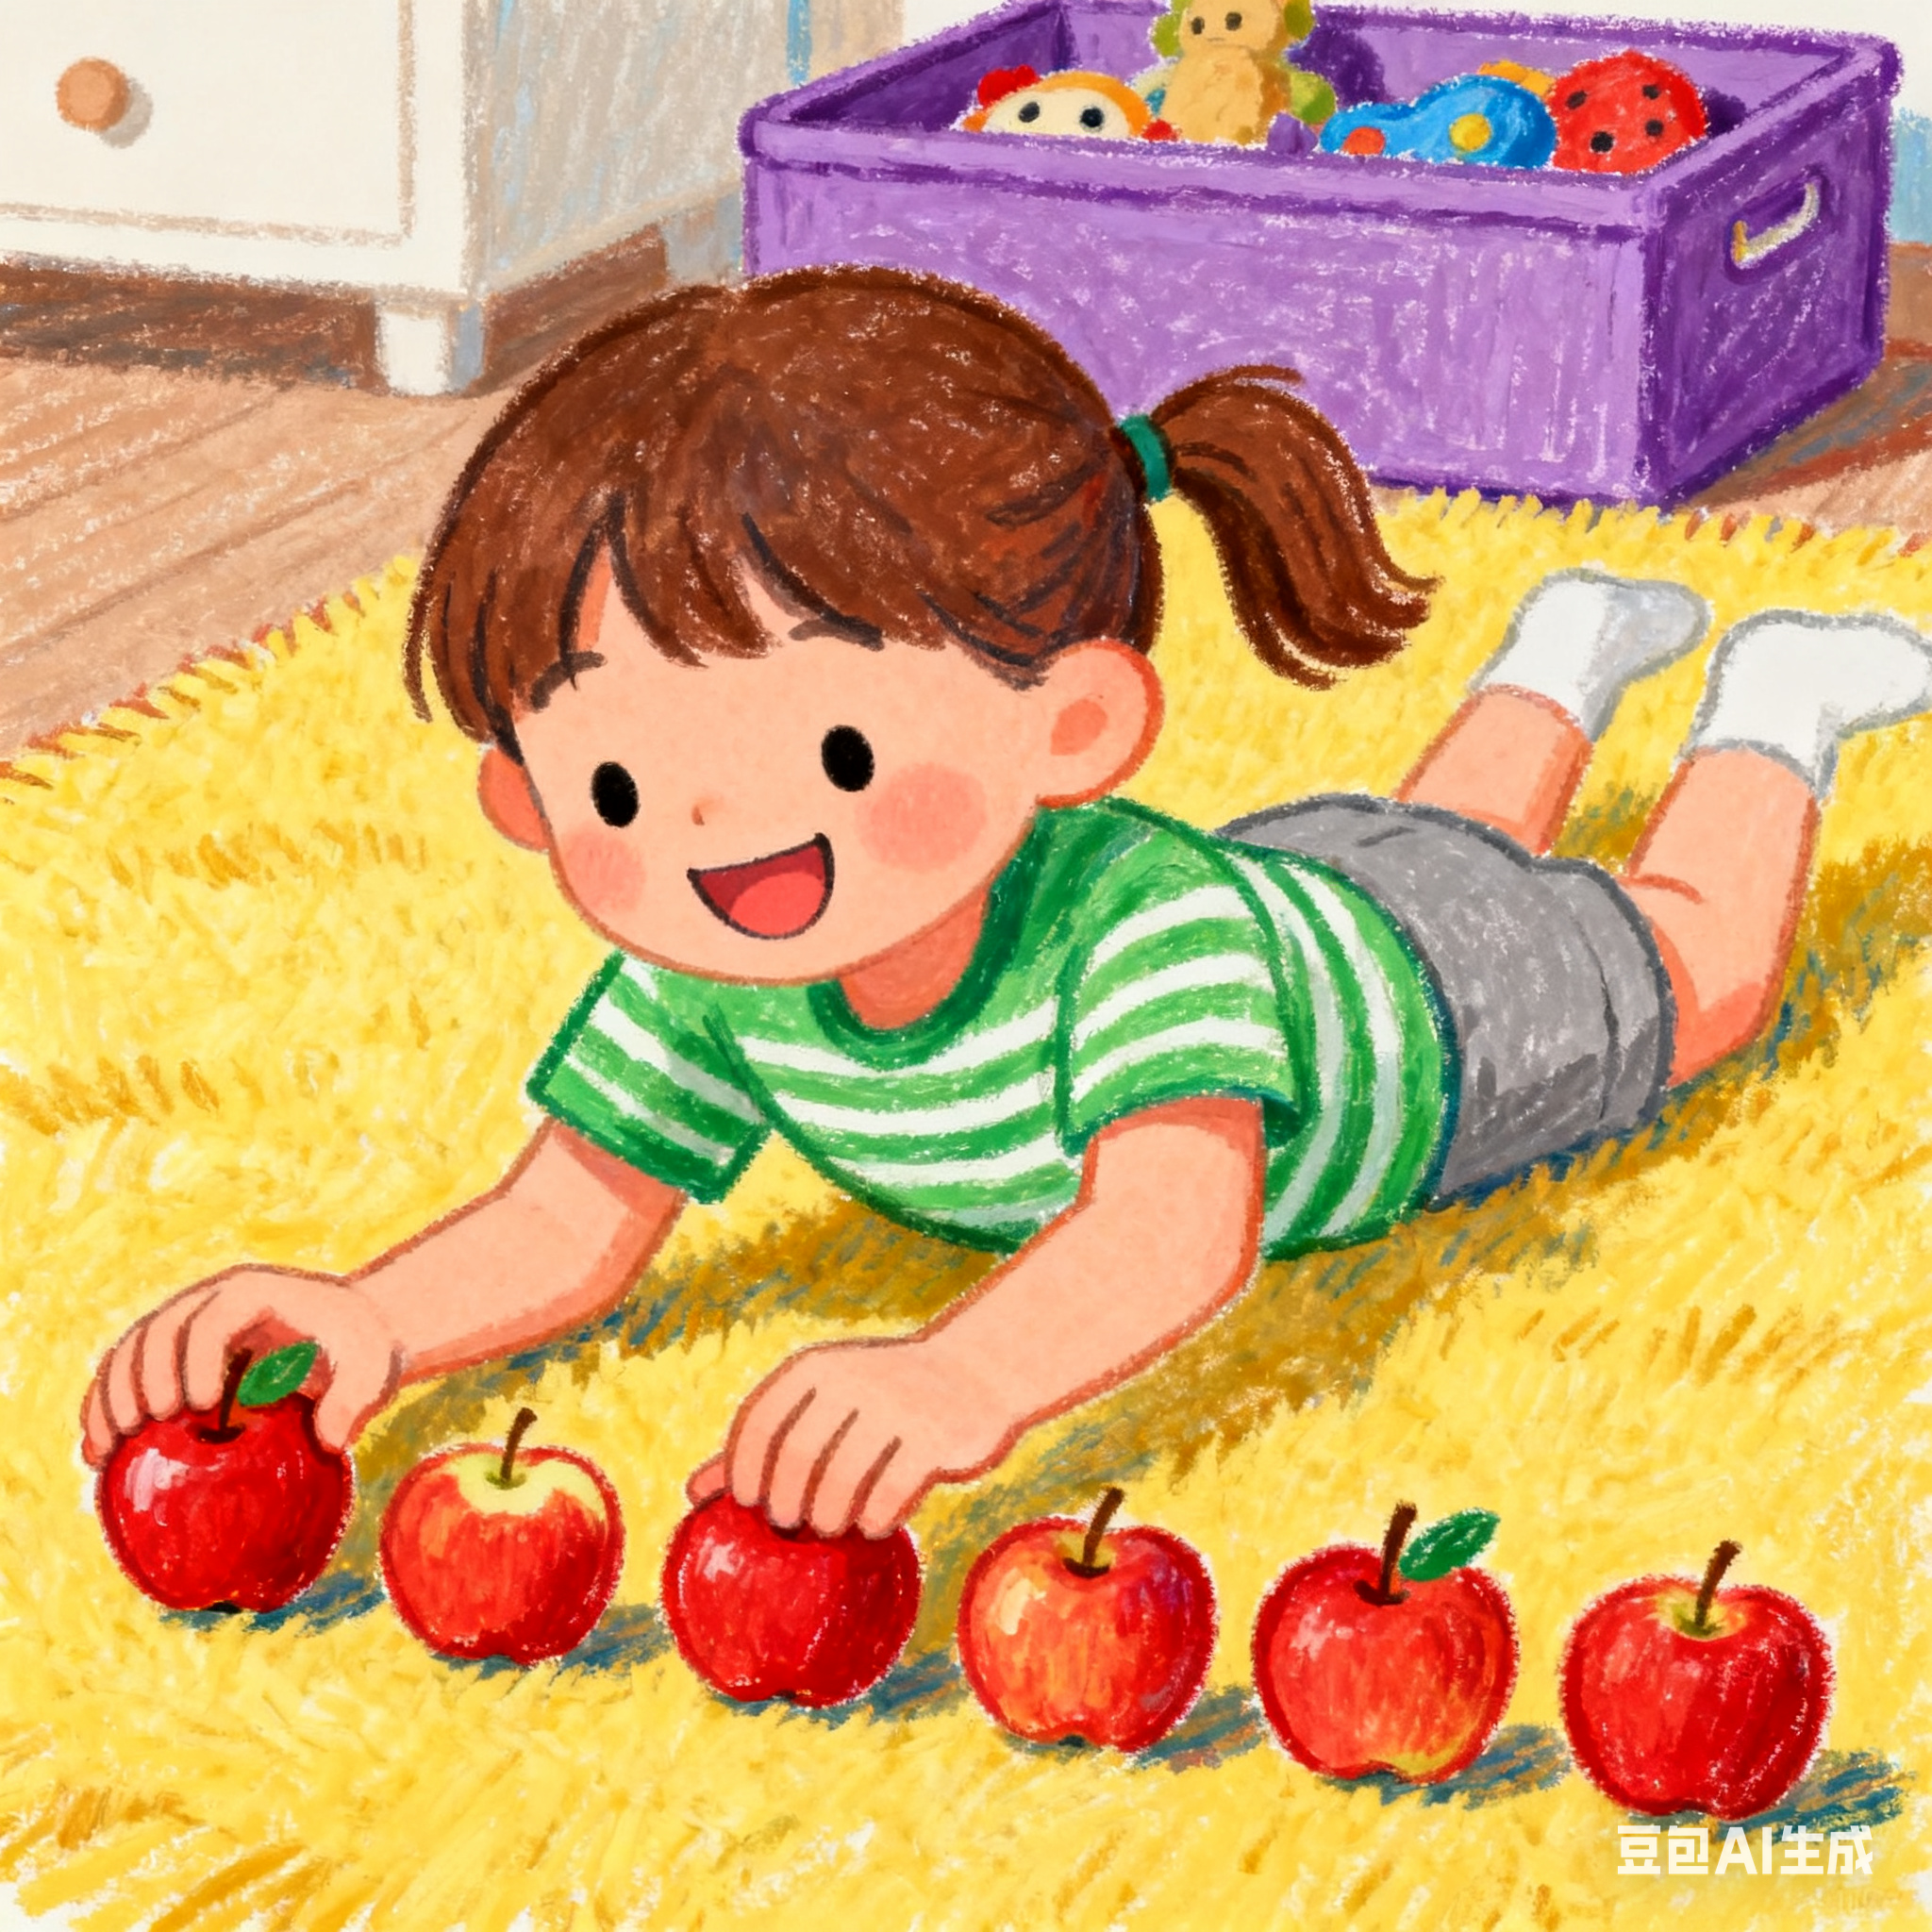
\includegraphics[width=0.8\textwidth]{countapple.png}
\paragraph{}如果是你,你可能会说:1, 2, 3, 4, \dots这样一直数,数出来的数就是自然数。
\paragraph{}我国高考遵循\textbf{国际标准 ISO 80000-2(the set of natural numbers, the set of positive integers and zero)}和\textbf{国家基础教育教材}的规范自然数包含0,那就是从0开始数,一直数出来数是自然数。
\paragraph{}说得没错,自然数就是你说的那些,而且只有那些,完全正确。
\section{再认识自然数}
\paragraph{}我现在化身杠精,想问问为什么从0开始数,数出来数是自然数,凭什么?老祖宗都说了:一生二,二生三,三生万物,从1数才是正解,才是自古以来。你只数到4,那5是不是自然数,9.9是不是自然数,很多是不是自然数,数不清是不是自然数......?总之,说从0数,数出来的数是自然数,我就是不服。
\subsection{从哪开始数}
\paragraph{}现在就0属不属于自然数,分为三个派别。第一个派别:传统派。认为0不属于自然数,这个派别应该是最古老的派别。你想,你数数会先数个0吗?会那么数的,C程序员无疑。打印字符串hello world!每个字符。
\begin{lstlisting}
	#include <stdio.h>
	int main() {
		char *str = "hello world!";
		
		for (int i = 0; str[i] != 0; i++) {
				printf("%c", str[i]);
		}
		return 0;
	}
\end{lstlisting}
\paragraph{}后来呢,像我这种懒人,偏听偏信的懒人多了,就发展出第二种派别:骑墙派。数数是从1开始数,那时候我是传统派。老师说高考定义是从0开始数,那时我就不是传统派。主打一个其乐融融,不惹事。
\paragraph{}那为什么把0加入到自然数,变成现在的正统了呢?那就要说到最后一个派别:集合论和逻辑学派。这个派别敬仰古希腊的荣光;就如同谈到西方政治,必然会有罗马帝国的痕迹。不论是希特勒第三帝国的建筑、艺术,还是美国政治人物的傲慢、自负,都似乎带着向罗马帝国致敬的味道,认为自己是伟大历史的书写者。古希腊的理性、思辨是人类的第一次觉醒,它塑造了现代文明:理性主义(不偏听偏信)、人文主义(生而平等)、公民意识(一切归劳动者所有,哪能容得寄生虫!)。看到上面说的是不是热血沸腾,会不会感觉古希腊的荣光还不够亮。
\paragraph{}\includegraphics[width=0.8\textwidth]{liberty_leading_people.png}
\paragraph{}一帮做数学的,也年轻过,也中二过,他们认为开创历史不是梦。他们从古希腊继承了有一部传世之作《几何原本》。我们作为普通人生活在距离这本书2300年后的今天,生活中99\%的数学问题,都可以从中找到解决方法。这本书让人惊叹的地方是:它只依赖5 条公理(适用于所有学科的基本真理,如 “等于同量的量彼此相等”)和 5条几何公设(如“过两点能作且只能作一直线”“直角都相等”),也就是只要承认5条公理5条几何公设,通过严格的逻辑推导,必然能够证明 465 个命题,它涵盖平面几何、立体几何、数论等领域。

% 公理部分
\begin{tcolorbox}[theorembox, title={5条公理}]
	\begin{enumerate}[label=\arabic*., leftmargin=*, noitemsep]
		\item 等于同量的量相等。
		\item 等量加等量,其和相等。
		\item 等量减等量,其差相等。
		\item 重合的量相等。
		\item 整体大于部分。
	\end{enumerate}
\end{tcolorbox}

\vspace{10pt} % 两个框之间的间距

% 公设部分
\begin{tcolorbox}[theorembox, title={5条公设}]
	\begin{enumerate}[label=\arabic*., leftmargin=*, noitemsep]
		\item 从任一点到任一点可以引一条直线。
		\item 有限的直线可以无限延长。
		\item 以任一点为中心,任意距离可以画圆。
		\item 所有直角都相等。
		\item 若一条直线与两条直线相交,且在同侧的两个内角之和小于两个直角,则这两条直线无限延长后,会在该侧相交。
	\end{enumerate}
\end{tcolorbox}
\paragraph{}于是集合论和逻辑学派的那帮人就思考,他们能不能也从几条基础的公理出发,根据逻辑推导最后重新建立数学大厦。
\paragraph{}初高中可能学了集合,可是会有种感觉:集合也就那么回事,好像什么事也没发生。对了,这种感觉对了。集合如果不和逻辑发生关系,它什么都不是。正是有了推导,才会有新的发现,美妙的启发。大部分的人的推导需要逻辑的约束,少部分人是不需要,比如女朋友、女朋友们、女朋友们的闺蜜们”。
\paragraph{}很多人说我也学过逻辑啊,辩证法不是逻辑吗?辩证法是我评价问题,指导行动的逻辑;所有的事物和变化发展规则都是对立统一、两个方面螺旋运动,内外力共同作用的结果。我要说的是:bi你bi的狗屁,但凡有人让你辩证的看待某个问题时,那他开始要不讲道理了。对(真)就是对(真),错(假)就是错(假),幼儿园老师、父母就是这样教的。bi人放火,打家劫舍就是错的,还辩证个屁。世界只有真和假,没有半真半假、即真又假。即真又假是岳不群、林平之。(这段话钟毅康表示不赞同、反对,但对于我个人观点给予尊重)
\paragraph{}学了逻辑后,有些人假话说得比真话多,学习让那些人变得狡猾。知道吗?说假话让你怎么说都是有对的地方;而说真话有一半的概率,会是错的。
\paragraph{}\underline{说假话,然后得出假的结论},别人会说:你说得好有道理。比如:
\begin{align}
	& 1 + 1 = 3 & \text{假条件} \label{c01:1}\\
	& (1 + 1)_3 + 1 = 3 + 1 & \text{\ref{c01:1}两边加1} \label{c01:2} \\
	& 3 + 1 = 4  & \text{\ref{c01:2}右边计算加法}
\end{align}
如果1+1=3,那么3+1=4,没错吧。
\paragraph{}\underline{说假话,然后得出对的结论},别人会说:你说得没错,赞。比如:
\begin{align}
	& 1 + 1 = 3  & \text{假条件} \label{c01:3}\\
	& \quad \ \ 0 = 1      & \text{\ref{c01:3}两边减2} \label{c01:4}\\
	& 1 + 1 = 2  & \text{\ref{c01:3}两边减\ref{c01:4}的两边}
\end{align}
如果1+1=3,那么1+1=2,没错吧。
\paragraph{}也就是,说假的前提,你怎么说都能给圆回去。古训说的:一句谎言,十句圆谎;十句谎言,一生难偿。古训欺负老实人嘛。
\paragraph{}说真话,必须得到真的结论,不然一下就穿帮了。比如你说1+1=2的话,1+1+1=4。别人会说:睁眼说瞎话嘛。
\paragraph{}既然这么容易被耍,后来人们就想了个办法,就是把结论当前提,看能不能圆回去(下图P$\Leftrightarrow$Q)。成功降低了被骗的概率。
\begin{table}[ht]
	\centering
	\caption{逻辑推导真值表}
	\label{tb:reduce}
	\begin{tabular}{cccccc}
		\toprule
		$P$ & $Q$ & $P \Rightarrow Q$ & $\neg$Q $\Rightarrow$ $\neg$P & $P \Leftrightarrow Q$ \\
		\midrule
		T & T & T & T & T \\
		T & F & F & F & F \\
		F & T & T & T & F \\
		F & F & T & T & T \\
		\bottomrule
	\end{tabular}
\end{table}
\paragraph{}$\iff$是个两头都有箭头的符号,箭头代表推导;$\Rightarrow$(向右的箭头)表示左边的情况如果满足,那么右边必然也满足;同理$\Leftarrow$(向左的箭头)表示右边情况满足,左边必然也满足。T表示真,F表示假,$\neg$表示反转。
\paragraph{}查看\eqref{tb:reduce},发现了一个规律,就是P$\Rightarrow$Q和$\neg$Q$\Rightarrow$$\neg$P,它们的真假值是一样的,一个命题和它的逆否命题真假一致。这个方法非常重要,当证明一个问题时,正面攻克不了,就攻克它的逆否命题。不过对于我这种“地瓜”智商,正面攻克不了,逆否也是白搭。我主要用这种方法写小作文,因为搞文学的人和小女生都喜欢这种不好好说的话。比如“我爱你”,变成命题形式:如果有个人是我,那么这个人爱你,现在改成逆反命题:如果一个人不爱你,那么,这个人不是我。经过逆否命题一改,字多了,诚意也多;这么绕,能把他们绕晕。逆反命题值得一练。
\begin{table}[ht]
	\centering
	\caption{非的真值表}
	\label{tb:neg}
	\begin{tabular}{cccccc}
		\toprule
		$P$ & $\neg$P \\
		\midrule
		T & F \\
		F & T \\
		\bottomrule
	\end{tabular}
\end{table}
\paragraph{}集合是把一类东西放一起,就像放学排入队,一群学生站一起;一堆苹果放一个货架上。放一起的东西各式各样,那取个名字吧,叫\underline{元素}。其实把元素叫东西也可以,但刚好集合的是一群人,叫东西就有些侮辱人了。干脆叫元素,反正你也没听说过,挑不出我毛病。
\paragraph{}看,多完美,我只是定义了一个框和东西,我们就可以开始数数了。等等,从哪里开始数呢,一开始集合里就有东西吗,有多少?数学家就想:从哪里开始数呢?就像《几何原本》它的需要5条公理5条公设,那数学需要的基础也是越少越好,难怪说数学家有洁癖。专业的人一般对自己的专业会有洁癖,表现得专业。比如我就看不惯函数4层以上的嵌套,goto乱来。洁癖和犟种的区别是,犟种不是蠢就是自卑。洁癖的数学家说:干脆从什么都没有开始,多干净。这个意见获得了数学家的共识。于是一条公理被提了出来:存在不含任何元素的集合。也就是别吵了,从0开始数。
\subsection{数学语言}
\paragraph{}这里插播一下。大部分人上大学后会发现,大学的数学书看不懂了。那其实是,近代数学公理化之后,同行之间开始用黑话交流。

{\itshape
“天王盖地虎,宝塔镇河妖”:这是《林海雪原》中最经典的黑话对答,是杨子荣假扮土匪时与座山雕手下的接头暗号。
“天王盖地虎” 意为 “你好大的胆子,敢来欺辱你祖宗?”
“宝塔镇河妖” 意为 “我若撒谎,让我被河水淹死,受宝塔镇压。”
“西北玄天一朵云,乌鸦落在凤凰群”:形容自己人来到了厉害的团伙中,下句接 “满桌都是英雄汉,谁是君来谁是臣?” 用于试探地位。

这是现代互联网里的黑话:我们要从顶层设计出发,聚焦用户痛点,通过差异化策略和精细化的颗粒度运营,击穿用户心智,打造产品的核心竞争力。在这个过程中,要注重各个环节的拉通和对齐,形成完整的业务闭环。同时,以数据为抓手,进行抽离透传和归因分析,为决策提供有力支持,不断赋能业务发展,最终实现业务的持续增长,在行业中构建起我们的生态优势。
}

看到互联网黑话,我就倒胃恶心;能不能好好说话!用模糊、新概念掩盖自己空洞,掩盖自己对具体问题毫无处理方法。一句话就是:无能。数学是由最聪明的一群人推动的,它的黑话不是无能,而且为了应对杠精,从源头把傻缺给排除。所以没有刻意训练数学的语言,当然是看不懂近代数学。好好学习这门语言吧,它会比英语更加通用,流传会更加悠远。更重要的是,学好后,你有资格和村口的大妈华山论剑,一决高下。

\begin{mdframed}[
	linewidth=1pt
	]

\quad \quad 我们说:元素、集合

老外说:element、set

数学说:我用小写字母a、b、x等表示元素,用大写字母A、B、C等或者用\{\}表示集合;而空集如此特殊,被定义为这个符号:$\emptyset$。
\end{mdframed}
\paragraph{}$\emptyset$是象形文字,用圆圈表示围起来的集合,用斜线划去表示什么都没有。例如一个包含a、b、c元素的集合A:\{a、b、c\}。
\begin{center}
	\begin{tcolorbox}[
		colback=white,
		colframe=blue!50!black,
		arc=3mm,
		boxrule=1pt,
		width=0.7\textwidth, % 框的宽度
		center, % 框内内容居中
		enlarge left by=0mm,
		enlarge right by=0mm,
		top=3mm,
		bottom=3mm,
		]
		空集公理:存在不含任何元素的集合。
		
		数学语言:$\exists$$\emptyset$$\forall$x(x $\notin$ $\emptyset$)
	\end{tcolorbox}
\end{center}
\paragraph{}上面的数学语言就是那批向古希腊致敬的数学家发明的,为了表达颠覆他们时代的意味,集合论里大部分成对关系的符号是倒影,或者是正常符号的翻转,空集公理的数学语言里有两个符号是正常符号翻转得来的。发现了吗:$\exists$、$\forall$。
\paragraph{}$\exists$左右旋转后是E,它源自拉丁语Existere的第一个字母。“Existere” 在拉丁语中由前缀 “ex-”(意为 “出、向外”)和词根 “sistere”(意为 “站立、存在”)组成,英语的exist(存在)就是这么来的。这个符号表的意思是:我就光明正大的站在这里。一般我们把他读作“存在”。存在就存在,有什么用呢?用处非常大,行走江湖抬杠必备。比如有人说:鸟都会飞。你说:存在一种鸟不会飞:鸵鸟。有人说:食物都会变馊。你说:存在一种食物不会变馊:蜂蜜。学会了吧,但凡别人说全部都怎么样,你只要举出$\exists$(存在)的一种反例,就能把他怼死。这就是$\exists$(存在)存在的意义。
\paragraph{}有认识$\forall$的朋友说:$\forall$是A的上下旋转,因为$\forall$的意思是“所有的”,那就是All的第一个字母。意思是对的,很可惜,来历不是这样的。它确实是所有的意思,但它是由拉丁语 “Omnis”(意为 “所有的、每一个”)的第一个字母得来的。我也无法理解$\forall$怎么就是O的旋转了,直到我看到o的手写体,为了连笔,o的左右俩边都有一个向下的线,上下旋转后变成向上的线,就变成了$\forall$。 $\forall$的目的是扩大打击面,就像《破坏之王》里的空手道大师兄“断水流”的经典台词:我不是针对你,我是说,在座的各位$\forall$都是勒色。又比如:你指出某些东西的不好,这时有人就说:\underline{任何}说**不好,$\forall$都是*黑。一般$\forall$可以用:“都”、“全部”、“任何一个、任意拿出一个”来表述,用“任何一个、任意拿出一个”表述最自然,最接近我们日常表达。
\paragraph{}上面的空集公理就还剩下最后一个符号了。$\notin$很明显那条斜线就是否定的意思,去掉斜线后是$\in$。$\in$源于拉丁语 “est”(某物是某集合的元素,即 “某物属于某集合”),这个单词和英语的“is”同一个意思。但我们不能简单的翻译成“是”,因为我们的“是”是等同的意思,而数学中,这个符号更准确的意思是“属于”、“是集合中的元素”。这个符号表示了元素和集合的关系。x$\in$A:x是A集合里的元素。x$\notin$A:x不是A集合里的元素。这里有个小细节,加上这个小细节,空集公理的数学语言我们就完全可以读懂了。这个细节是我们把可以改变的元素,用x、y、z这种小写字母表示,而用a、b、c这种小写字母表示不会改变的元素。
\paragraph{}重读空集公理:$\exists$$\emptyset$$\forall$x(x $\notin$$\emptyset$)。直译:存在空集和所有的元素,所有的元素都不属于空集。再译:存在空集和所有元素,从所有元素中取出任何元素,这个元素都不属于空集。说人话就是:存在空集,空集里不包含任何元素。
\paragraph{}好啦,废话一堆。目的就是说:从空集公理出发,我们的自然数从0开始数。空集里没元素,没有任何东西,我们就说空集表示0。
\subsection{我会数数了}
\paragraph{}有0了,那1是不是也要定义一个区别$\emptyset$的集合,叫1集合?为了遵循“如无必要,勿增实体”的原则,死犟死犟的数学家什么都没引入,他把空集再用了一遍来表示1。我想到的是这种\{$\emptyset$\}。漂亮!这种表示1,无懈可击。接着来2,\{$\emptyset$、$\emptyset$\}。
\paragraph{}嗯......这个2的集合表示好像碰到了点问题。什么问题呢?举个例子:把家庭成员里,会打乒乓球的人组成一个集合,这个集合是A:\{我、弟弟\};把家庭成员里,是程序员的人组成一个集合,这个集合是B:\{我\}。现在把家庭成员里,会打乒乓球的人和程序员组成一个集合C。这个集合C是\{我、弟弟\},还是\{我、弟弟、我\}呢?很明显,看上去它们是有区别的,但实质上它们描述的是同一个事物。也就是集合中相同的元素即使重复多次,对集合的整体没有影响。
\paragraph{}那2到底要如何从上面仅有的元素、集合、空集的概念推导出来呢?$\emptyset$和$\emptyset$是同一个,然而$\emptyset$和\{$\emptyset$\}不是同一个。那2就可以用\{$\emptyset$、\{$\emptyset$\}\}表示。
\paragraph{}到这,我似乎发现了获得下一个集合的规律。把当前集合元素的所有元素合并到下一个集合,再加上一个“当前集合”的元素(集合作为元素)。
\begin{itemize}[label=]
	\item 0:$\emptyset$ $\rightarrow$ 把$\emptyset$作为下一个集合的元素
	\item 1:\{$\emptyset$\} $\rightarrow$ \underline{\{$\emptyset$\}}
	\item 2:\{$\emptyset$、\underline{\{$\emptyset$\}}\} $\rightarrow$ \underline{\{$\emptyset$、\{$\emptyset$\}\}}
	\item 3:\{$\emptyset$、\{$\emptyset$\}、\underline{\{$\emptyset$、\{$\emptyset$\}\}}\} $\rightarrow$ \underline{\{$\emptyset$、\{$\emptyset$\}、\{$\emptyset$、\{$\emptyset$\}\}\}}
\end{itemize}
\paragraph{}漂亮,后面的4、5、6\dots 不是问题了,按照规则数下去都能得到。 
\subsection{先填一个坑}
\paragraph{}首先要填的第一个坑就是:明明可以用一次加一个$\emptyset$的方式来创造自然数,也就是集合里有1个空集,表示1,两个空集表示2的这种方式来表示自然数。为什么舍近求远,你不能用“我是我,独一无二的我”这个口号来灌输我错误的观念,说得好听,我是被卖家秀骗过的人,我要解释!很遗憾,没法给出解释,真没办法给出解释。
\paragraph{}数学家对没办法解释的事物,处理办法相当简单粗暴。没办法解释是吧,那就提出一个公理:
\begin{center}
	\begin{tcolorbox}[
		colback=white,
		colframe=blue!50!black,
		arc=3mm,
		boxrule=1pt,
		width=0.9\textwidth, % 框的宽度
		center, % 框内内容居中
		enlarge left by=0mm,
		enlarge right by=0mm,
		top=3mm,
		bottom=3mm,
		]
		外延公理:两个集合的元素相等,那么这两个集合相等。
		
		数学语言:$\forall X \forall Y (\forall x (x \in X \iff x \in Y) \iff X = Y)$
	\end{tcolorbox}
\end{center}
\paragraph{}说实话,我一看到外延公理,我的第一反应是什么鬼。我说的不是,我不能理解外延公理的内容,而是“外延”这个词。“外延”是什么?能不能取个一目了然的名字:元素公理。等我带着这个问题,查看了“外延(extension)”、“内涵(intension)”的意思才知道,这两个词是一对,而且它们是哲学词汇。集合论的创立者“康托”在大学学习的是数学和哲学,那就难怪这公理的名字怪哲学,不是凡人可以明白。简单的说:“内涵”是我们的描述;“外延”是根据描述,能得到的东西。就例如:小于4的自然数是内涵,外延是\{0、1、2、3\}。从内涵你就能得出外延,但从外延不一定能得到你要的内涵。例如从外延\{0、1、2、3\},有人认为是小于4的自然数,有人认为是前4个自然数。使用内涵表示集合,甚至引发悖论,罗素悖论是个很有名的内涵悖论的例子。从上面的解释可以看出,要获得准确的、直接的信息,应该提取的是外延。在集合里,也就是元素。

{\itshape
有一个很有名的内涵悖论:罗素悖论。
	\begin{itemize}[label=$\bullet$]
		\item 某理发师宣称:“我只给所有不给自己理发的人理发。”	
		\item 请问:这个理发师该不该给自己理发。
		\begin{itemize}[label=$\circ$]
			\item 若他给自己理发,则违反 “不给自己理发” 的原则;
			\item 若他不给自己理发,则根据原则应给自己理发。
		\end{itemize}
	\end{itemize}
}
\paragraph{}接着来看看数学语言,有了上面学习数学语言的基础,重读外延公理:任意的两个集合A和B,任何的一个元素,只要这个元素在A里,那么这个元素必然也在B里;只要这个元素在B里,那么这个元素必然也在A里。那么我们说集合A等于集合B。倒回来,任意的两个集合A、B,A等于B,那么A的所有元素在B里,B的所有元素在A里。
\paragraph{}如果认为\{$\emptyset$\}代表1,\{$\emptyset$、$\emptyset$\}代表2,利用外延公理可以推导出1=2的悖论。
\begin{proof}
	把\{$\emptyset$\}记作X,把\{$\emptyset$、$\emptyset$\}记作Y。
	\begin{itemize}[label=]
		\item  \{$\emptyset$\}的所有元素是$\emptyset$。满足$\emptyset$ $\in$ \{$\emptyset$、$\emptyset$\};即$\forall$x(x$\in$X $\Rightarrow$ x$\in$Y)。
		\item \{$\emptyset$、$\emptyset$\}的所有元素是$\emptyset$、$\emptyset$。第一个$\emptyset$满足$\emptyset$ $\in$ \{$\emptyset$\},第二个$\emptyset$满足$\emptyset$$\in$ \{$\emptyset$\};即$\forall$x(x$\in$X $\Leftarrow$ x$\in$Y)。
		\item 根据外延公理:$\forall X \forall Y (\forall x (x \in X \iff x \in Y) \iff X = Y$。
		\item 得证\{$\emptyset$\} = \{$\emptyset$、$\emptyset$\}
	\end{itemize}
\end{proof}
所以根据配对公理,用\{$\emptyset$、$\emptyset$\}表示2不是可取的方法。
\subsection{再填一个坑}
\paragraph{}回顾上面说的创造下一个集合的规律:是把当前集合元素的所有元素合并到下一个集合,再加上一个“当前集合”的元素(集合作为元素)。

\begin{itemize}[label=]
	\item 0:$\emptyset$ $\rightarrow$ 把$\emptyset$作为下一个集合的元素。
	\item 1:\{$\emptyset$\} $\rightarrow$ \underline{\{$\emptyset$\}}
	\item 2:\{$\emptyset$、\underline{\{$\emptyset$\}}\} $\rightarrow$ \underline{\{$\emptyset$、\{$\emptyset$\}\}}
	\item 3:\{$\emptyset$、\{$\emptyset$\}、\underline{\{$\emptyset$、\{$\emptyset$\}\}}\} $\rightarrow$ \underline{\{$\emptyset$、\{$\emptyset$\}、\{$\emptyset$、\{$\emptyset$\}\}\}}
\end{itemize}
\paragraph{}首先要解决的第一个问题:两个集合必然能组成一个集合。这是我们从空集出发创造新集合做的第一个动作,我们需要把它合法化。遇事不决,出公理:
\begin{center}
	\begin{tcolorbox}[
		colback=white,
		colframe=blue!50!black,
		arc=3mm,
		boxrule=1pt,
		width=0.9\textwidth, % 框的宽度
		center, % 框内内容居中
		enlarge left by=0mm,
		enlarge right by=0mm,
		top=3mm,
		bottom=3mm,
		]
		配对公理:任意的两个集合a、b能组成新的集合C=\{a、b\}。
		数学语言:$\forall$a $\forall$b $\exists$C $\forall$x(x $\in$ C $\iff$ (x = a $\lor$ x = b))
	\end{tcolorbox}
\end{center}
\paragraph{}读数学语言:这句数学语言出现了新的符号:$\lor$,它读作“或”、“或者”。它的来源是拉丁语“vel”(或)的首写字母v。记不住的话,就把$\lor$当成一个坑,或者这个或者那个都可以往里边丢。它的用法是只要$\lor$的左右两边有一个有效就认为“$\lor$左右两边”这个整体有效。比如别人问你:什么时候踢进世界杯?你可以回答:草坪太干或者草坪太湿或者草坪不干不湿,我都会输球。说得输球好像不是你的问题,是草坪的问题。草坪那么多或者的情况,只要满足一条,你就可以输球。用数学的语言把配对公理读出来就是:任意两个集合(两个形成配对,所以叫配对公理),存在第三个集合,第三个集合里的任何一个元素是前面两个集合之一。
\paragraph{}配对公理只是解决了两个集合能组成第三个集合,而且第三个集合里的元素是前两个集合。我们通常把这种“集合的元素是集合”的集合称为集合族。其实应该叫集合群,也就是一群集合组成的集合,但群在数学已经被伽罗瓦提前占位了,族群、族群,只剩下族了,所以我们把这类集合叫集合族。虽然两个集合组成第三个集合已经合法化,但我们通常更加关注的是把前两个集合的元素打散放到第三个集合,也就是合并两个集合的元素。
\begin{center}
	\begin{tcolorbox}[
		colback=white,
		colframe=blue!50!black,
		arc=3mm,
		boxrule=1pt,
		width=0.9\textwidth, % 框的宽度
		center, % 框内内容居中
		enlarge left by=0mm,
		enlarge right by=0mm,
		top=3mm,
		bottom=3mm,
		]
		并集公理:存在一个集合,它的元素是集合族里集合的元素。
		
		数学语言:$\forall$X $\exists$Y $\forall$u(u $\in$ Y $\iff$ $\exists$z(z $\in$ X $\land$ u $\in$ z))
	\end{tcolorbox}
\end{center}
\paragraph{}读数学语言:这里又出现了一个数学符号$\land$,它刚好和我们从配对公理学的$\lor$方向相反。$\lor$是或者的意思,相反的$\land$是而且的意思。比如很多男人说的“肤白貌美大长腿”,是或者的意思,只要有一个满足就是美女;很多女人说的“有车有房”才结婚,是而且的意思,必须有车而且有房,都达到了才满足条件。严以律己、宽以待人说的是对自己要用而且,对别人要用或者。现在这句古训慢慢被另一句话替代:我也是第一次做人,凭什么?先通读一遍$\forall$X $\exists$Y $\forall$u(u $\in$ Y $\iff$ $\exists$z(z $\in$ X $\land$ u $\in$ z)),从z $\in$ X $\land$ u $\in$ z可以看出来,X是一个集合族,因为X的元素是z,而z的元素是u,也就是z是一个集合,X的元素是集合z。有了这些信息,从头开始读:任何的集合族,都存在一个集合,这个集合的元素是集合族里集合的元素。
\begin{definision}
	集合的并运算 X $\cup$ Y 定义为:
	\[
	X \cup Y = \{ x \mid x \in X \lor x \in Y \}
	\]
\end{definision}
集合的并,就是把集合的所有元素提取出来,放入新的集合作为元素。现在可以让我们根据配对公理和并集公理,构造从0 $\rightarrow$ 1 $\rightarrow$ 2 $\rightarrow$ 3了。
\begin{itemize}[label=]
	\item 0:$\emptyset$
	\item 1:\{$\emptyset$\} $\rightarrow$ \underline{\{$\emptyset$\}}
	\item 2:\{$\emptyset$、\underline{\{$\emptyset$\}}\} $\rightarrow$ \underline{\{$\emptyset$、\{$\emptyset$\}\}}
	\item 3:\{$\emptyset$、\{$\emptyset$\}、\underline{\{$\emptyset$、\{$\emptyset$\}\}}\} $\rightarrow$ \underline{\{$\emptyset$、\{$\emptyset$\}、\{$\emptyset$、\{$\emptyset$\}\}\}}
\end{itemize}
\paragraph{}构造从0 $\rightarrow$ 1。有两个集合$\emptyset$、\{$\emptyset$\},根据并集公理,必然有一个集合,这个集合的元素是两个集合的元素。$\emptyset$没有元素,\{$\emptyset$\}的元素是$\emptyset$,所以构造的集合是\{$\emptyset$\}。
\paragraph{}构造从1 $\rightarrow$ 2。有两个集合\{$\emptyset$\}、\{\{$\emptyset$\}\},根据并集公理,必然有一个集合,这个集合的元素是两个集合的元素,\{$\emptyset$\}集合的元素是$\emptyset$,\{\{$\emptyset$\}\}集合的元素是\{$\emptyset$\},所以构造的集合是\{$\emptyset$、\{$\emptyset$\}\}。
\paragraph{}构造从2 $\rightarrow$ 3。有两个集合\{$\emptyset$、\{$\emptyset$\}\}、\{\{$\emptyset$、\{$\emptyset$\}\}\},根据并集公理,必然有一个集合,这个集合的元素是两个集合的元素,\{$\emptyset$、\{$\emptyset$\}\}的元素是$\emptyset$、\{$\emptyset$\},\{\{$\emptyset$、\{$\emptyset$\}\}\}的元素是\{$\emptyset$、\{$\emptyset$\}\},所以构造的集合是\{$\emptyset$、\{$\emptyset$\}、\{$\emptyset$、\{$\emptyset$\}\}\}
\paragraph{}根据上面的方法,就可以一直的构造自然数。从现在开始,我宣布“你可以合法的数数了”。
\subsection{填最后的坑}
\paragraph{}从上面构造自然数,我们采用了一种方法构造下一个自然数的方法:$x^{+} = x \cup \{x\}$。这种方法有个名称叫:\underline{归纳}。我们在生活中还经常碰到一个词:递归。递归就像内卷,当整个社会产生了内卷的氛围,这种氛围就像病毒一样蔓延到每个公司,公司再把这个病毒传递给每员工,员工又在不知不觉中传递到家庭,又从家庭传递给每一个人。递归是一种简单的方法,但它能触及到任何的角落。作为程序员可以不知道归纳,但万万不能不知道递归。程序的函数是指把一个过程组合成一个整体可以操作的对象。递归是在这个函数过程中,再次执行了这个函数。例如你要获取计算机所有的文件名称,下面的几行递归伪代码实现了这个目的。
{\itshape
	\begin{itemize}[label=]
		\item 遍历目录(需要遍历的目录路径) \{
		\begin{itemize}[label=]
			\item 打开需要遍历的目录路径
			\item 查看当前层级的文件和目录
			\item 如果是文件,那么收集这个文件名称
			\item 如果是目录,那么再次执行\large{遍历目录(这个目录路径)}
		\end{itemize}
		\item \large{遍历目录(我的电脑)}
	\end{itemize}
}
\paragraph{}\underline{递归采用的是从大往小递进;归纳正好相反,它是从小往大延伸。}仔细观察,生活中处处有递归和归纳,只要是一种能渗透进每个角落的传播方式,那它不是递归就是归纳,或者是两者震荡放大的结果。扶不扶摔倒的老人是归纳,买不买房是递归,内卷是从几家IT公司开始(You are shame)归纳到IT行业竞争氛围,然后通过氛围递归到整个社会。
\paragraph{}说了这么多,现在思考一个问题:归纳是一个过程,这个过程在自然数中是不会停止的,那需要怎么看待自然数。简单的说:把自然数看出一个过程,还是一个整体。也就是自然数是不是一个集合。小白会疑惑,这重要吗?当然,这关系到1 $\div$ 3 = 0.33$\dot{3}$ 里的0.33$\dot{3}$,你认为它是一个 真实存在的确切的数,还是一个过程。为了解决这个问题,再次提出了一个公理:
\begin{center}
	\begin{tcolorbox}[
		colback=white,
		colframe=blue!50!black,
		arc=3mm,
		boxrule=1pt,
		width=0.9\textwidth, % 框的宽度
		center, % 框内内容居中
		enlarge left by=0mm,
		enlarge right by=0mm,
		top=3mm,
		bottom=3mm,
		]
		无穷公理:存在由归纳产生的集合。
		
		数学语言:$\exists$S [$\emptyset$ $\in$ S $\land$ ($\forall$x $\in$ S)[x $\cup$ \{x\} $\in$    S]]
	\end{tcolorbox}
\end{center}
\begin{definision}
	$x^+ = x \cup \{x\}$,把$x^+$读作x的后继。以数字作为符号,定义后继:
	\[
		0^+ = 1 \quad 1^+ = 2 \quad 2^+ = 3 \quad \cdots
	\]
\end{definision}
\paragraph{}用数学语言读无穷公理:存在一个集合,空集是这个集合的元素,而且这个集合的元素的后继也是这个集合的元素。也就是从这个无穷公理开始,数学归纳法才真正合法。思考数学归纳法的步骤:命题的首项满足,如果命题的第n项满足的条件下,命题的第n项的后继也满足,那么我们说命题对全部($\forall$)自然数项满足。
\paragraph{}既然自然数是一个集合,而且这么重要的集合出去闯江湖。碰上鼠辈放肆,大吼一声:江湖道义岂容尔等践踏,藏头露尾非英雄,本人行不更名,坐不改姓,人称$\mathbb{N}$,Natural numbers的$\mathbb{N}$。一声枪响,$\mathbb{N}$卒,弹幕:“$\mathbb{N}$死于话多,下次别废话了!”
\section{有趣的自然数}
\paragraph{}我感觉这个章节,会很困惑,因为我们现在只有归纳一个工具,而且第一次讨论无穷。无穷它的一些性质颠覆了我们的很多固有想法,这个章节我们一块思考无穷情况下的问题。
\paragraph{}首先我们先做一个约定,我们接下来讨论的都是函数问题。当别人和你说:我们做个约定吧。这时请别光想着约定的美,还附带要放弃一部分自由呢。这里约定讨论函数问题,不仅仅是放弃我的自由,更重要的是我的智商只能勉强思考函数的问题。所以有些时候,放弃部分自由,其实是在保护自己。\dotuline{函数}问题之所以说简单,是因为它要求根据特定的输入,经过运算输出的\dotuline{结果只有一个},它非常符合认知。对于结果、目的、输出你不能既要又要。有一个结果就够了,只有围城内的才知道“一夫一妻”其实是在保护男性。既要又要的结果就是,没办法预测结果。函数的一个要求就是,结论,或者说输出唯一。这个唯一不是任何输入对应的输出的确切结果唯一,说的是在确定输入的情况下结果唯一。比如身份证,一个身份证号对应唯一的一个人,其他人的身份证号不对应这个人,指向其他的唯一的人。函数简单的说就像进动车站刷身份证,输入身份证信息和你的人脸,经人证合一的校验,输出唯一的结论:是你或者不是你,来决定让不让你进站。根据以上的分析,函数包含三个方面:输入非、运算、输出。而且特别要求,根据指定的输入,对应的输出是唯一的。
\begin{definision}
	函数是输入集合对应输出集合的一种关系,输入集合的一个元素,唯一地输出集合的一个元素。下列的符号定义F()表示函数运算,x表示输入,y表示输出。
	
	F(x, y):$\forall$x $\forall$y$_{1}$ $\forall$y$_{2}$[(f(x, y$_{1}$) $\in$ F $\land$ f(x, y$_{2}$) $\in$ F) $\Rightarrow$ y$_{1}$ = y$_{2}$]
\end{definision}
有了函数,我们就可以定义运算了。首先我们想到的是什么?当然是加、减、乘函数。
有了函数还不够,因为我们关注的是自然数的函数。我们现在只有一个自然数集合,一个集合是无法满足函数的条件,需要两个集合输入集合和输出集合。那么现在我们需要从自然数分离出一个集合。由前面给的所有知识,都无法分离出一个集合,所以提出新的公理。
\begin{center}
	\begin{tcolorbox}[
		colback=white,
		colframe=blue!50!black,
		arc=3mm,
		boxrule=1pt,
		width=0.9\textwidth, % 框的宽度
		center, % 框内内容居中
		enlarge left by=0mm,
		enlarge right by=0mm,
		top=3mm,
		bottom=3mm,
		]
		分离公理:可以从任何集合中提取满足制定性质的元素,组成新的集合。
		
		数学语言:$\forall$A $\exists$B $\forall$x(x $\in$ B $\iff$ x $\in$ A $\land$ P(x))
	\end{tcolorbox}
\end{center}
\paragraph{}有了分离公理,我们可以提取自然数的数构成输入集合和输出集合。然后只剩下确保输出的唯一性,也就是归纳的输出要唯一。回顾归纳方法:$x^{+}=x\cup\{x\}$,做个假设,如果有一个集合它的元素是它自己,那么根据归纳方法和外延公理,归纳方法就会终结。
\paragraph{}因为我们不希望集合后继还是集合自己,所以我们需要确保:集合的元素不能是集合自己。
\begin{equation}
\textit{集合的元素不能是这个集合自己,即A $\neq$ \{A\}。} \notag
\end{equation}
\begin{Proof}
	用反证法证明:如果集合的元素还是集合自己,那么集合的后继还是自己。\\
	集合的元素还是集合自己:
	\begin{align}
		A&=\{A\} &&\quad \label{eq:selfcontained}
	\end{align}
	后继的定义:
	\begin{align}
		A^{+}&=A\cup\{A\} &&\quad \label{eq:successor}
	\end{align}
	把 \eqref{eq:selfcontained} 代入 \eqref{eq:successor}得到:$A^{+} = A \cup A$,根据集合的并运算和外延公理得到,得到$A^{+}=A$。
\end{Proof}
为了避免这个情况出现,再、再、再、再次提出一个公理。呜呜......数学越来越不美了,一碰到问题,就出一个公理,简直就是bug一般的存在。还能比黑人和原住民后代,性别认知障碍又有异装癖,素食又环保主义者buff叠满更无敌吗。
\begin{center}
	\begin{tcolorbox}[
		colback=white,
		colframe=blue!50!black,
		arc=3mm,
		boxrule=1pt,
		width=0.9\textwidth, % 框的宽度
		center, % 框内内容居中
		enlarge left by=0mm,
		enlarge right by=0mm,
		top=3mm,
		bottom=3mm,
		]
		正则公理:任意非空集合含有一个与自身不相交的元素。
		
		数学语言:$\forall$X(X $\neq$ $\emptyset$ $\Rightarrow$ $\exists$x(x $\in$ X $\land$ X $\cap$ x = $\emptyset$))
	\end{tcolorbox}
\end{center}
前面刚学了集合的并$\cup$,这里的$\cap$刚好是$\cup$的翻转,这两个符号是一对,$\cap$叫集合的交,$\cup$是把集合所有元素都提取出来组成新的集合;$\cap$是把两个集合\underline{相同}的元素提取出来组成新的集合。
\paragraph{}所以根据归纳方法和外延公理,集合符合正则公理的前提下,归纳不会终结,而且归纳产生的元素,是这个归纳集中独一无二的元素。对应自然数而言,自然数集合中的自然数个数是无穷的,每个自然数在自然数集合中独一无二。
\begin{definision}
	集合的交运算 X $\cap$ Y 定义为:
	\[
	X \cap Y = \{ x \mid x \in X \land x \in Y \}
	\]
\end{definision}
正则公理英文是Axiom of Regularity/Foundation,翻译英文叫规范公理或者基础公理。这里的规范和基础,说的是集合的规范和基础。
\paragraph{}根据正则公理$A \neq \{A\}$,那么$A^{+} \neq A \cup \{A\}$。对应到自然数:$x \neq x^{+}$,也就是自然数集合中的数与这个数的后继不相等。
\subsection{我会加法、乘法了}
\label{subsec:addmul} 
当我推理到有自然数的概念后。我认为可以这样解释加法:a+b是在自然数a的基础上执行b次的后继。是的,加法确实是以这种方式定义的。
\begin{definision}
	自然数的加法表示符合下列规则的函数$f_{+}$或者$f_{add}$,其中$x \in \mathbb{N} \land y \in \mathbb{N}$:
	\begin{empheq}[left=\empheqlbrace]{align}
		& x + 0 = x \tag{df.add.1}\label{df:add1} \\
		& x + y^{+} = (x + y)^{+} \tag{df.add.2}\label{df:add2}
	\end{empheq}
\end{definision}
这个定义表述得非常自然。一个任意数x加上另一个数,\eqref{df:add1}是任意数x加上另一个数的起点,然后反复\eqref{df:add2}的后继运算。例如我要算x+2。
\begin{align}
	x + 0 &= x & \quad \text{根据\eqref{df:add1}} \label{add:0}\\
	x + 1 &= (x + 0)^{+} = x^{+} & \quad \text{根据\eqref{df:add2}\eqref{add:0}} \label{add:1}\\
	x + 2 &= (x + 1)^{+} = ((x + 0)^{+})^{+} = (x^{+})^{+} & \quad \text{根据\eqref{df:add2}\eqref{add:1}}
\end{align}
上面的推导中,依赖数字作为符号的后继定义$0^{+}=1$、$1^{+}=2$。
\paragraph{}这个加法定义困扰了我很久,因为它有太多的问题值得思考:首先加法后的结果,能保证还是自然数吗?毕竟减法就产生了负数,除法产生了有理数,加法是如何保证运算后的结果在自然数范围内呢?其次加法符合函数的性质吗?也就是加后的结果唯一吗?
\paragraph{}到现在,我们的自然数还用着集合的、归纳的“表示”,“表示”是没用的,多少心爱的人都是被表示给耽误了。偷偷地看对方,她会认为我就是那么好看,别人也这样看她;酸溜溜的说:他是不是喜欢你。她会认为你打探她的隐私。直到你说,三十岁你还没结婚,我们凑合过吧。她暴怒,你在诅咒老娘嫁不出去是不是。表示不一定有用,也许别人认为你在养鱼。所以到了确定关系的时候了,大胆表白,不做舔狗。舔狗舔狗,添到最后一无所有。该给自然数下个定义了。
\paragraph{}这个定义是皮亚诺给的,也叫作皮亚诺公理,是公认的自然数的公理,满足下面皮亚诺公理的集合叫自然数集合$\mathbb{N}$,集合里的元素叫自然数。为了强调$x^{+}$的后继是一个数,后续会用S(x)表示$x^{+}$。另外新学一个逻辑符号$\exists$!,它的意思是“有且唯一”,中国有且唯一,大陆属于中国,台湾属于中国:$\exists$!中国(大陆$\in$中国 $\land$ 台湾$\in$中国)。有了$\exists$!这个符号,那么我们可以给出函数定义的简化版本:$\forall$x$\exists$!y(f(x,y) $\in$ F)。
\begin{enumerate}[label=\textbf{P\arabic*.}] 
	\item \textbf{0是自然数}($0\in\mathbb{N}$)。
	\item \textbf{每个自然数x,有唯一的S(x),S(x)也是自然数}($\exists!S(x)(x\in\mathbb{N} \land S(x)\in\mathbb{N})$)。
	\item \textbf{0 不是任何自然数的后继}($\forall x(x\in \mathbb{N} \land S(x) \neq 0)$)。
	\item \textbf{不同的自然数有不同的后继}($\forall x \forall y ((x \in \mathbb{N} \land y \in \mathbb{N} \land x \neq y) \Rightarrow S(x) \neq S(y))$)。
	\item \textbf{数学归纳法}:如果某个性质P满足:
	\begin{enumerate}
		\item P(0)成立,
		\item P(n) $\Rightarrow$ P(S(n)),\\
		则P对所有自然数成立。
	\end{enumerate}
\end{enumerate}
\paragraph{}皮亚诺公理可以由前面介绍的公理系统严格推导出来,例如P1和P3的简单推导:
\paragraph{}P1:由无穷公理定义$\mathbb{N}$,0=$\emptyset$,0是$\mathbb{N}$的一个元素。
\paragraph{}P3:如果0是某个自然数x的后继,那么0=x$\cup$\{x\}。0=$\emptyset$,根据配对公理、并集公理和外延公理只有x=$\emptyset$和\{x\}=$\emptyset$,但是x=$\emptyset$和\{x\}=$\emptyset$是矛盾的。
\paragraph{}明确了自然数的定义后,我们现在可以考虑第一个问题:自然数加法的结果能保证还是自然数吗?
\begin{equation}
	\textit{自然数加法的结果还是自然数} \label{nor:addstnor}
\end{equation}
\begin{Proof}
	根据加法规则($x \in \mathbb{N} \land y \in \mathbb{N}$):
\begin{empheq}[left=\empheqlbrace]{align}
	& x + 0 = x \tag{df.add.1}\label{df:add1} \\
	& x + y^{+} = (x + y)^{+} \tag{df.add.2}\label{df:add2}
\end{empheq}
\paragraph{}从\eqref{df:add1}可以看出来,这个规则已经帮我们解决了n=0的情况。
\paragraph{}当n=0时
\begin{align}
	x + n &= x + 0 & \quad \text{当n = 0} \label{add:n0}\\
	x + 0 &= x     & \quad \text{根据\eqref{add:n0}\eqref{df:add1}} \label{add:x0}\\
	(x + 0) &\in \mathbb{N} & \quad \text{根据$x \in \mathbb{N}$和\eqref{add:x0}} \label{add:y3}
\end{align}
\paragraph{}当n $\neq$ 0时,\itshape{归纳假设}:
\begin{equation}
	(x + n) \in \mathbb{N} \label{add:y0}  
\end{equation}
\paragraph{}证明($x+S(n)) \in \mathbb{N}$:
\begin{align}
	x + S(n) &= S(x + n) & \quad \text{根据\eqref{df:add2}}  \label{add:y1}\\
	S(x+n) &\in \mathbb{N} & \quad \text{根据\eqref{add:y0}和皮亚诺公理P2}  \label{add:y2}\\
	(x + S(n)) &\in \mathbb{N} & \quad \text{根据\eqref{add:y2} \eqref{add:y1}}  \label{add:y4}
\end{align}
\paragraph{}\eqref{add:y3}结论说明P(0)成立,\eqref{add:y0}和\eqref{add:y4}说明P(n) $\Rightarrow$ P(S(n))成立,由皮亚诺P5得出自然数x加上任意的自然数n,加出来的结果依然是自然数。
\end{Proof}
接着第二个问题:加法算出来的结果唯一吗?因为这直接关系到,加法是不是一个函数问题。
\begin{equation}
	\textit{自然数加法的结果唯一} \label{nor:addres1}
\end{equation}
\begin{Proof}
当n=0时
\begin{align}
	x + n &= x + 0 & \quad \text{当n = 0} \label{add:y15} \\
	x + 0 &= x     & \quad \text{根据\eqref{add:y15}\eqref{df:add1}} \label{add:y16}
\end{align}
\paragraph{}当n $\neq$ 0时,\itshape{归纳假设}:
\begin{equation}
	(x + n) \text{结果唯一} \label{add:y17}
\end{equation}
\paragraph{}证明(x + S(n))的结果唯一。
\begin{align}
	x + S(n) &= S(x + n) & \quad \text{根据\eqref{df:add2}} \label{add:y18} \\
	S(x + n) & \text{结果唯一} & \quad \text{根据\eqref{add:y17}和皮亚诺公理P2} \label{add:y19} \\
	(x + S(n)) & \text{结果唯一} & \quad \text{根据\eqref{add:y18}\eqref{add:y19}} \label{add:y20}
\end{align}
\paragraph{}\eqref{add:y16}结论说明P(0)成立,\eqref{add:y17}和\eqref{add:y20}说明P(n) $\Rightarrow$ P(S(n))成立,由皮亚诺P5得出自然数x加上任意的自然数n,加出来的结果是唯一的。
\end{Proof}
\paragraph{}第三个问题:是否存在一个除0外的自然数x,自然数n加上x后还是n?
\begin{equation}
	\textit{任意自然数n加上有且仅有0,还是n} \label{add:eq00}
\end{equation}
\begin{Proof}
	\begin{align}
		& \text{重述问题:n + x = n 是否为真} & \text{$x \in \mathbb{N}, n \in \mathbb{N}, (x \neq 0)$} \label{eq:nxn} \\
		& \text{$S(n + x) = S(n)$} & \text{根据\eqref{eq:nxn}和皮亚诺P2} \label{eq:nxn1} \\
		& \text{$n + S(x)$ = n + 1} & \text{根据\eqref{df:add2}\eqref{add:1}} \label{eq:nxn2} \\
		& \text{$S(0) = 1$} &\text{根据自然数定义}\label{eq:nxn3} \\
		& \text{$n + S(x)$ = n + S(0)} & \text{根据\eqref{eq:nxn2}\eqref{eq:nxn3}} \label{eq:nxn4} \\
		& \text{x = 0} & \text{根据\eqref{eq:nxn4}} \label{eq:nxn5} \\
		& \text{x = 0 \eqref{eq:nxn5}和x $\neq$ 0\eqref{eq:nxn}相矛盾} \label{eq:nxn6}
		\end{align}
根据证明得到:
	\begin{align}
			& \text{$n + x \neq n$} & \text{$x \in \mathbb{N}, n \in \mathbb{N}, (x \neq 0)$} \label{eq:nxn7}
	\end{align}		
\end{Proof}
\paragraph{}第四个问题:
\[
\begin{cases}
	a = b \\
	c = d
\end{cases}
\textit{是否可以$\implies$} a + c = b + d  \quad \text{($a, b, c, d \in \mathbb{N}$)}
\]
\begin{Proof}
证明a = b 则a + c = b + c。
\paragraph{}当c=0时
\begin{align}
	& \text{a + 0 = b + 0} & \text{根据\eqref{df:add1}}
\end{align}
\paragraph{}当c$\neq$0时,归纳假设:
\begin{equation}
	a = b \Rightarrow a + c = b + c \label{co:add1}
\end{equation}
\paragraph{}证明 a + S(c) = b + S(c)
\begin{align}
    & \text{a + S(c) = S(a + c)} & \text{根据\eqref{df:add2}} \label{co:add2} \\
    & \text{b + S(c) = S(b + c)} & \text{根据\eqref{df:add2}} \label{co:add3} \\
    & \text{S(a + c) = S(b + c)} & \text{根据\eqref{co:add1}和皮亚诺公理P4} \label{co:add4} \\
    & \text{a + S(c) = b + S(c)} & \text{根据\eqref{co:add2}\eqref{co:add3}\eqref{co:add4}}
\end{align}
证得
\begin{align}
\begin{cases}
	a = b \\
	c = d
\end{cases}
\text{$\implies$} a + c = b + d  \quad \text{($a, b, c, d \in \mathbb{N}$)} \label{co:add5}
\end{align}
\end{Proof}
\paragraph{}学会了加法,现在我们可以参加小学一年级期末考试啦,祝200个月的小朋友考试顺利。考试及格,欢迎加入乘法的学习。
\begin{definision}
	自然数的乘法表示符合下列规则的函数$f_{\times}$或者$f_{mul}$,其中$x \in \mathbb{N} \land y \in \mathbb{N}$:
	\begin{empheq}[left=\empheqlbrace]{align}
		& x \times 0 = 0 \tag{df.mul.1}\label{dmul:1} \\
		& x \times S(y) = x \times y + x \tag{df.mul.2}\label{dfmul:2}
	\end{empheq}
\end{definision}
\paragraph{}乘法也具有加法的函数性质,证明方法是一样的,我就不证明了。总结:自然数加法和乘法是自然数集合通过加法和乘法规则运算,映射到自然数集合的函数。直接给出以下结论:
\begin{equation}
	\textit{自然数乘法的结果还是自然数} \label{nor:mulnor}
\end{equation}
\begin{equation}
	\textit{自然数乘法的结果唯一} \label{nor:mulres1}
\end{equation}
\paragraph{}可以通过加法和乘法定义,以及数学归纳法证明以下运算规律:
\begin{align}
	x + y &= y + x & \quad \text{自然数加法交换律} \label{add:ex}\\
	(x + y) + z &= x + (y + z) & \quad \text{自然数加法结合律}  \label{add:asso}\\
	x \times y &= y \times x & \quad \text{自然数乘法交换律} \\
	(x \times y) \times z &= x \times (y \times z) & \quad \text{自然数乘法结合律} \\
	(x + y) \times z &= x \times z + y \times z \\
	 z \times (x + y) &= z \times x + z \times y  & \quad \text{自然数分配律}  \label{addmul:dis}
\end{align}
\begin{convension}
	当使用单个字母表示数时,它们的乘法可以简写为:$\cdot$或者直接省略。
	\begin{align*}
		\text{例如:} a \times b = a \cdot b = ab
	\end{align*}
\end{convension}
\subsection{一样,多了,少了?}
\paragraph{}在1998年《新华字典》修订本中有这样一个例句:“张华考上了北京大学;李萍进了中等技术学校;我在百货公司当售货员:我们都有光明的前途。”当年12岁的我,读了这句话,明白了什么是相等。首先,我的前途是光明的,光明的前途是我的。其次,我把售货员的前途给张华,张华欣然接受;张华把上北京大学的前途给我,我可以接受。再次,我把售货员的前途给张华,张华把上北京大学的前途给李萍,李萍把进中等技术学校的前途给我,我们都很开心。把它们总结为数学语言就是:
\begin{definision}
	集合X上的二元关系R,具有以下性质的关系称为\underline{等价关系}:
	\begin{align}
		& \text{所有的$x \in X$都有xRx。} \tag{自反性} \label{df:eqreflerive} \\
		& \text{所有的$x, y \in X$都有$xRy \Rightarrow yRx$。} \tag{对称性} \label{df:eqsymmetric} \\
		& \text{所有的$x, y, z \in X$都有$(xRy \land yRz) \Rightarrow xRz$。} \tag{传递性} \label{df:eqtransitive}
	\end{align}
\end{definision}
等价关系虽然简单,但是它却可以帮助我们认识新的运算。例如这个集合\{(0, 4), (1, 3), (2, 2), (3, 1), (4, 0)\},它蕴含集合\{0, 1, 2, 3, 4\}里加法和是4的等价关系:(a, b)R(c, d) $\leftrightarrow$ a + b = c + d = 4。也就是通过等价关系,我们可以推导出部分自然数的一种加法运算。后面的章节,我们利用等价关系,结合运算推导出新的数。
\begin{definision}
	x的等价类:
	\begin{align*}
		\text{所有与x满足关系R的元素组成的集合,记作$[x]_{R}$或简写为$[x]$。} \label{df:equivalenceclass}
	\end{align*}
\end{definision}
上面的$[(0, 4)]$ = \{(0, 4), (1, 3), (2, 2), (3, 1), (4, 0)\}是集合\{0, 1, 2, 3, 4\}里加法和是4的等价类。偶数也可以是一个等价类:$[0]$=\{0, 2, 4……\}。
\paragraph{}只要是具有等价关系,那么它们是可以相互替换的。例如在计算加法时,会把2+2替换为0+4,或者是化简后的4;除了算数运算时的替换,在证明时也会有替换,例如证明(x + S(n)) $\in$ $\mathbb{N}$\eqref{add:y4},把x + S(n) = S(x + n)\eqref{add:y1}等价的算式代入到S(x + n) $\in$ $\mathbb{N}$\eqref{add:y2};在逻辑推理时也会采用等价的方法,例如根据逻辑推理真值表\eqref{tb:reduce},结合非得真值表\eqref{tb:neg},那么会有(P $\Rightarrow$ Q)和($\neg$Q $\Rightarrow$ $\neg$P)真假值等价,这种逻辑等价给我们提供了更多,灵活多变的推导方式。
\paragraph{}除了等价的二元关系,还有一种二元关系和日常息息相关,那就是搞排名,比大小。假设有一家科技公司,它的营销费用占营收10\%左右,假设另一家取消传统营销部门的公司,它的营销费用占营收0.16\%。你认为在现实中,取消传统营销的公司,在营收更高的情况下,谁还有更多的钱投入研发、产品质量?如果两家科技公司宣传时,一家除了宣传科技价值,还强调附带特别的情绪价值,另一家仅仅推广科技价值,请问哪家公司的科技排名更靠前?真像成绩排名不好的我,成绩不够文具来凑,“差生文具多”说的是我。
\paragraph{}上面这种关系是偏序关系,它最显著的特点就是舍我其谁,我最最厉害,另一个我都不能和我比。
\begin{definision}
	集合X上的二元关系R,具有以下性质的关系称为\underline{严格偏序关系}:
	\begin{align}
		& \text{所有的$x \in X$都有x\cancel{R}x。} \tag{反自反性} \\
		& \text{所有的$x, y, z \in X$都有$(xRy \land yRz) \Rightarrow xRz$。} \tag{传递性}
	\end{align}
	\cancel{R}的意思是不存在关系。
\end{definision}
\paragraph{}小于号$<$和大于号$>$是我们常用的严格偏序符号,用于比大小,长短,轻重,排名。自然数的大小刚好可以利用刚学的加法来定义。
\begin{definision}
	任意自然数a、b, 当且仅当($\iff$)以下条件,那么a $<$ b 和 b $>$ a:
	\begin{equation}
		a + x = b  \quad \quad \text{$\exists x(x \in \mathbb{N} \land x \neq 0)$} \label{df:compare} \tag{df.n.order}
	\end{equation}
\end{definision}
\paragraph{}定义了大于、小于你就正式告别快乐的童年了。这时你会发现,父母的眼里永远有一类小朋友。他成绩大于你,乖巧懂事大于你,惹是生非小于你,他是你无法逾越的鸿沟,父母、老师眼中的榜眼,他是舞台上的明星、红旗下的花朵。他有个响亮的名字:领居家的小孩。其实不用担心,因为你也可能是其他父母眼中的那个领居家的小孩。

\paragraph{}\textit{对任意m,n $\in \mathbb{N}$,以下三种情况有且只有一个成立:}
	\begin{equation}
		m < n \quad \quad m = n \quad \quad m > n \label{nor:sort3}
	\end{equation}
\begin{Proof}
	证明只会有一种情况成立:
	\begin{itemize}[label=$\circ$]
	\item 当m $<$ n时:
		\begin{align}
			& m + x = n \quad \text{$\exists x(x \in \mathbb{N} \land x \neq 0)$} \quad & \text{根据\eqref{df:compare}} \label{pf:t1}\\
			& m \neq n & \text{根据\eqref{pf:t1}\eqref{eq:nxn7}} \label{pf:t2} \\
			& \text{假设 m $>$ n,则n + y = m} & \text{根据\eqref{df:compare}} \label{pf:t3} \\
			& n + y + x = n & \text{根据\eqref{pf:t3}\eqref{pf:t1}} \label{pf:t4} \\
			& \text{n + y + x $\neq$ n} & \text{根据\eqref{eq:nxn7}} \label{pf:t5} \\
			& \text{m $\cancel{>}$ n} & \text{根据\eqref{pf:t4}和\eqref{pf:t5}矛盾}
		\end{align}
	\item 当m = n时:
	\begin{align}
		& \text{$n + x \neq m$} & \text{根据m=n和\eqref{eq:nxn7}} \label{pf:t6} \\
		& \text{m $\cancel{<}$ n} & \text{根据\eqref{pf:t6}\eqref{df:compare}} \\
		& \text{m $\cancel{>}$ n} & \text{根据\eqref{pf:t6}\eqref{df:compare}}
	\end{align}
	\item 当m $>$ n时:
		\begin{align}
		& n + x = m \quad \text{$\exists x(x \in \mathbb{N} \land x \neq 0)$} \quad & \text{根据\eqref{df:compare}} \label{pf:t7}\\
		& n \neq m & \text{根据\eqref{pf:t7}\eqref{eq:nxn7}} \label{pf:t8} \\
		& \text{假设 m $<$ n,则m + y = n} & \text{根据\eqref{df:compare}} \label{pf:t9} \\
		& m + y + x = m & \text{根据\eqref{pf:t7}\eqref{pf:t9}} \label{pf:t10} \\
		& \text{m + y + x $\neq$ m} & \text{根据\eqref{eq:nxn7}} \label{pf:t11} \\
		& \text{m $\cancel{<}$ n} & \text{根据\eqref{pf:t10}和\eqref{pf:t11}矛盾}
	\end{align}
	\end{itemize}
\paragraph{}必然存在三种情况之一,数学归纳法证明:
	\begin{itemize}[label=$\circ$]
	\item 当m = 0时:n 可以分成两种情况:n = 0和n $\neq$ 0;
		\begin{itemize}[label=]
			\item n = 0:
				\begin{align}
					& \text{m = n}	& \text{根据m=0, n=0}
				\end{align}
			\item n $\neq$ 0:
				\begin{align}
					& \text{0 + n = n} & \text{根据\eqref{df:add1}} \label{pf:t14} \\
					& \text{m + n = n} & \text{根据\eqref{pf:t14}和m=0} \label{pf:t15} \\
					& \text{m $<$ n} & \text{根据\eqref{pf:t15}\eqref{df:compare}}
				\end{align}
		\end{itemize}
	\item 当m $\neq$ 0时:
		\begin{itemize}[label=]
			\item 假设m = n, m $<$ n, m $>$ n必有一种情况成立。
			\item 分析m 与 S(n)的关系:
			\begin{itemize}[label=]
				\item m = n:
				\begin{align}
					& \text{n + 1 = S(n)} & \text{根据\eqref{eq:nxn2}} \label{pf:t17} \\
					& \text{m + 1 = S(n)} & \text{根据\eqref{pf:t17}和m=n} \label{pf:t18} \\
					& \text{m $<$ S(n)} & \text{根据\eqref{pf:t18}\eqref{df:compare}}
				\end{align}
				\item m $<$ n:
				\begin{align}
					& \text{m + x = n} & \text{根据m $<$ n和\eqref{df:compare}} \label{pf:t20} \\
					& \text{S(m + x) = S(n)} & \text{根据皮亚诺公理P3} \label{pf:t21} \\
					& \text{m + S(x) = S(n)} & \text{\eqref{pf:t21}\eqref{df:add2}} \label{pf:t22} \\
					& \text{m $<$ S(n)} & \text{根据\eqref{pf:t22}\eqref{df:compare}}
				\end{align}
				\item m $>$ n:则 n + k = m
				\begin{itemize}
					\item k = 1:
					\begin{align}
						& \text{n + 1 = m} & \text{根据条件} \label{pf:t23} \\
						& \text{n + 1 = S(n)} & \text{根据\eqref{add:1}} \label{pf:t24} \\
						& \text{m = S(n)} & \text{根据\eqref{pf:t23}\eqref{pf:t24}}
					\end{align}
					\item k $>$ 1:
					\begin{align}
						& \text{1 + x = k} & \text{根据\eqref{df:compare}} \label{pf:t25} \\
						& \text{n + 1 + x = m} & \text{根据条件和\eqref{pf:t25}} \label{pf:t26} \\
						& \text{S(n) + x = m} & \text{根据\eqref{add:1}\eqref{pf:t26}} \label{pf:t27} \\
						& \text{m $>$ S(n)} & \text{根据\eqref{pf:t27}\eqref{df:compare}}
					\end{align}
				\end{itemize}
			\end{itemize}
		\end{itemize}	
	\end{itemize}
\end{Proof}
\subsection{数一数,看谁多}
\paragraph{}自然数的严格偏序关系,为比较任意两个自然数大小,提供了很大方便。然而有些情况,这种方法就不好使了,需要返璞归真,回忆最初你是怎么比较大小的。
\paragraph{}小时候什么都会和弟弟比,多夹了一块肉,吵架多骂了一句笨蛋,都会沾沾自喜,觉得自己赢了,开心!看谁夹的肉多:你夹了一块,我也夹一块,我趁着弟弟不注意,偷偷再夹一块,而这时弟弟没夹,那我就比弟弟多了。吵架也是,弟弟说我一个笨蛋,我说一个反弹,只要他每个笨蛋都跟着我一个反弹,我们就没赢没输。但凡我少一个反弹,或者弟弟多一个笨蛋,都是我输了。这种比较多少的好处是两方不管有多少,只要双方一一对应,谁还有多,谁就是多的一方。
\paragraph{}比较多少这么简单,那比较一下,自然数里的偶数多还是奇数多。好啊,0是偶数,1是奇数,抵消掉;2是偶数,3是奇数,抵消掉;4是偶数,5是奇数,抵消掉……
\paragraph{}这样数数不行,数到天荒地老也数不完。重新梳理下,首先明确目的,再次详细过程。目的是比较自然数里的偶数和奇数,偶数是什么,奇数又是什么。偶数是能被2整除的数,奇数是不能被2整除的数。除没有学过,用乘重新定义自然数的偶数和奇数。
\begin{definision}
	自然数里的偶数:
	\begin{equation*}
		2 \times n  \quad \text{($n \in \mathbb{N}$)} \tag{df.n.eval} \label{n:eval} 
	\end{equation*}
\end{definision}
\begin{definision}
	自然数里的奇数:
	\begin{equation*}
		2 \times n + 1  \quad \text{($n \in \mathbb{N}$)} \tag{df.n.odd} \label{n.odd}
	\end{equation*}
\end{definision}
\begin{theorem}
自然数里的偶数和奇数一样多。
\end{theorem}
\begin{Proof}
	\begin{align}
		2 \times n + 1 &= S(2 \times n) & \quad \text{根据\eqref{add:1}} \label{eeqo:1}\\
		S(2 \times n) &= S(\text{自然数里的偶数}) & \quad \text{根据\eqref{eeqo:1} \eqref{n:eval}} \label{eeqo:2} \\
		\text{自然数里的奇数} &= S(\text{自然数里的偶数}) & \quad \text{根据\eqref{eeqo:1} \eqref{eeqo:2}} \label{eeqo:3}
	\end{align}
	\begin{equation}
		\text{根据\eqref{eeqo:3}和皮亚诺公理P2,自然数里的偶数和奇数一样多。} 
	\end{equation}
\end{Proof}
\paragraph{}自然数里的偶数和奇数一样多,还是比较容易接受的,毕竟自然数就是由自然数里的偶数和奇数组成的,一半一半很合理。那我要说,自然数里的偶数和自然数一样多呢?
\paragraph{}部分和整体一样多,是不是疯了?如果真有部分和整体一样多的东西,我希望是钱。如果10块钱里拿出5块钱,5块钱变成10块钱那么多,我花掉原来的5块钱(10-5),还有10块钱(5块钱变的10块钱)。想想都美滋滋,可以躺平,吃喝等死了。部分和整体一样多,怎么可能?可是数学是不会骗人的,再看看偶数的定义\eqref{n:eval},任何一个自然数n都能生成一个自然数里的偶数(2$\times$n),所有自然数里的偶数(2$\times$n)都能由自然数n生成。所以自然数里的偶数和自然数一样多。
\paragraph{}我们把集合里的元素个数称为基数。集合里的元素个数有限,它的基数是自然数中的一个数。例如集合{a, b, c},它的基数是3。如果集合元素个数和自然数个数一样多,就把基数读作阿列夫0($\aleph_{0}$)。上面的例子,两个集合可以通过函数把两个集合的每个元素一一对应起来,很容易证明两个集合的基数相等。如果要比较更复杂一点的集合基数,例如两个集合的基数都是阿列夫0($\aleph_{0}$),现在在其中一个集合中加上100个元素,那么它们的基数还相等吗?就像两个绝世高手,会降龙十八掌的乔峰对上练易经筋的庄聚贤(游坦之)。这时候,乔峰加了主角光环,他们谁输谁赢?
\paragraph{}要解决复杂问题,需要再次整理思路,结合集合和数学逻辑,从新认识一一对应。首先两个集合,集合A和集合B;其次集合A的任意一个元素只对应集合B中的一个元素;最后集合B中的元素都可以被集合A中的元素对应上。我们结合函数用数学符号语言表示一一对应,然后只要证明符号语言每个部分都是有效的,也就证明了两个集合一一对应。
\begin{definision}\label{dff:bijection}
	两个集合元素一一对应:
	\begin{align*}
		& \exists f(f(A, B) \land S1 \land S2) \tag{双射} \label{df:bijection} \\
		& \quad S1: \forall a_{1},a_{2} \in A(f(a_{1}) = f(a_{2}) \Rightarrow a_{1} = a_{2}) \tag{单射} \label{df:One-to-One} \\
		& \quad S2: \forall b \in B \exists a \in A(f(a) = b) \tag{满射} \label{df:Onto}
	\end{align*}
\end{definision}
\begin{definision}
	集合A能和集合\{0, 1, 2\dots n\}一一对应,那么说集合A是有限集,A的基数都是n-1,记作:
	\[
	|A| = n + 1
	\]
\end{definision}
\begin{definision}
	A 是有限集 $\iff$ 存在一个自然数 n(包括 0),使得 $|A|$=n
\end{definision}
\begin{definision}
	不是有限集的集合是无限集。自然数集合的基数是阿列夫0($\aleph_{0}$)。
\end{definision}

\paragraph{}两个集合的基数都是阿列夫0($\aleph_{0}$),现在在其中一个集合中加上100个元素,比较它们的基数是否还相等。
\begin{Proof}
	只要两个集合元素能一一对应,那么它们的基数是相等的。根据\eqref{df:bijection},只要函数满足\eqref{df:One-to-One}和\eqref{df:Onto}即可。
	\paragraph{}可以假设两个集合它们是A:\{$a_{0}, a_{1}, a_{2}$……\},B:\{$b_{0}, b_{1}, b_{2}$……\},加入的100个元素到B,那么B:\{$c_{0}, c_{1}, c_{3}$……$c_{99}, b_{0}, b_{1}, b_{2}$……\}。
	可以有这样的一个函数:
		\begin{empheq}[left=\empheqlbrace]{align}
		& f(a_{i}) = c_{i}  & \quad \text{$0 \leq i <100$}  \label{pf:bj1}\\
		& f(a_{i}) = b_{i-100}  & \quad \text{$i \geq 100$} \label{pf:bj2}
	\end{empheq}
	\begin{itemize}[label=$\circ$]
		\item 单射: 推导$f(a_{x})=f(a_{y}) \Rightarrow a_{x}=a_{y}$ \label{pf:bj3}
		\begin{itemize}[label=]
			\item 当0 $\leq$ i $<$ 100:
			\begin{align}
				& \text{$f(a_{x}) = c_{x}$ 和 $f(a_{y}) = c_{y}$} & \text{根据\eqref{pf:bj1}} \label{pf:bj4} \\
				& \text{$c_{x} = c_{y}$} & \text{根据$f(a_{x})=f(a_{y})$和\eqref{pf:bj4}} \label{pf:bj5} \\
				& \text{x = y} & \text{根据\eqref{pf:bj5}和$c_{i}$唯一} \label{pf:bj6} \\
				& \text{$a_{x} = a_{y}$}
			\end{align}
			\item 当i $\geq$ 100:证明步骤同上,略。
		\end{itemize}
		\item 满射:集合B的元素由$c_{0}, c_{1}, c_{3}$……$c_{99}$和$b_{0}, b_{1}, b_{2}$……组成。
		\begin{itemize}[label=]
			\item 根据\eqref{pf:bj1},任意一个$c_{x}$存在$a_{x}$。
			\item 根据\eqref{pf:bj2},任意一个$b_{x}$存在$a_{x+100}$。
		\end{itemize}
	\end{itemize}
\end{Proof}
\begin{definision}
	集合A的元素都是集合B的元素,那么说集合A是集合B的子集。A:\{x $| x \in$ B\} $\Rightarrow$ A $\subseteq$ B。
\end{definision}
\begin{theorem}
	有最大值的自然数子集是有限集
\end{theorem}
\begin{Proof}
	构造集合 S=$\{x \in \mathbb{N} | x \leq M\}$。由自然数的定义可知:S=$\{0, 1, 2 \dots M\}$,根据有限集的定义集合S是有限集,$|S|$=M+1。
	\paragraph{}设命题的集合是T,根据命题T $\subseteq$ S。由于集合T的元素都属于集合S,那么T的元素数量不会大于S的元素数量,所以$|T| \leq |S|$。$|S|$=M+1,那么$|T| \leq M+1$。也就是集合B的元素个数是一个不大于M+1的自然数,所以T是有限集。
\end{Proof}


\chapter{可单位度量的数}
\paragraph{}前两个小节(减法,负数)(除法,分数)非常无聊,它们的内容是利用自然数对,在加法规则和乘法规则下,构造负数和分数。其他的小节可以看看,或许有你喜欢的内容。
\paragraph{}学习,思考过自然数后,可以开始总结“数”包含哪些关键的东西,怎样构造新的数。我们思考:自然数有哪些值得关注的东西。首先,自然数是一个\{0,1,2……\}的集合;其次,构造自然数的方法:0和后继;再次,然数有加法和乘法的运算法则;最后,自然数有等价和严格偏序。我们可以把以上的总结,组成一个集合,这个集合叫数集。一个数集包含最关键的是这些信息:数字的集合,关系,运算法则,特殊数字。自然数集可以表示为:\{$\mathbb{N}$,\{+$\times$\},\{=$<$$>$\},{0}\}。
\paragraph{}我一直以为是减法创造了负数,除法创造了分数,根号创造了无理数。渐渐地我改变了这种观点,运算法则最多是启发,创造谈不上。新的数集的创造是观念、思想上的突破,全部的负数、分数能用减法、除法运算获得,但全部的实数确不能用某个运算获得。从离散的数到完备的实数,从能力有限的黎曼积分到完备的勒贝格积分,都是观念、思想上的突破。这样看,减法和负数的关系,除法和分数的关系更像是一种美丽的巧合。
\section{负数}
\subsection{定义整数}
\paragraph{}既然学了等价类,那我们根据加法,数对的等价类集合来表示自然数:
\begin{align*}
	\mathbb{N} = \{&\{(0, 0)\}, \\
	&\{(0, 1), (1, 0)\}, \\
	&\{(0, 2), (1, 1), (2, 0)\} \\
	&\{(0, 3), (1, 2), (2, 1), (3, 0)\} \\
	& \cdots\}
\end{align*}
从上面的自然数枚举可以看出来,通过数对结合加法运算法则也是可以遍历自然数。例如第一行数是数对,和是0的等价类,第二行是数对,和是1的等价类,第三行是数对,和是2的等价类。我们希望这些数对能兼容其他的运算法则和运算规律。以3$\times$7为例:
\begin{align*}
	3 \times 7 &= 21 \\
	(1 + 2) \times (3 + 4) &= 1 \times (3 + 4) + 2 \times (3 + 4) \\
	                       &= 7 + (2 \times 3 + 2 \times 4) \\
	                       &= 7 + 14 \\
	                       &= 21
\end{align*}
很棒!数对保持了自然数的运算法则和运算规律,当然这是由加法和乘法的运算法则和规律保证的(\eqref{add:ex} $\sim$ \eqref{addmul:dis})。
\paragraph{}继续观察,交换两个数对里元素的顺序,是否有新的发现,以7等价的数对为例:(5, 2)、(4, 3)。
\begin{equation}
	[(5, 2) \quad (4, 3)] \quad \underline{\text{交换数对后项}} \rightarrow \quad [(5, 3) \quad (4, 2)]
\end{equation}
\paragraph{}交换数对后项后的数对是(5, 3) (4, 2)。发现可以给数对里的数存在相同的大于关系,5 $>$ 3、4 $>$ 2。根据大于的定义:3 + 2 = 5, 2 + 2 = 5。好像有点意思了,总结是:两个等价数对(例如(5, 2)和(4, 3))后项交换,得到新数对(例如:(5, 3)和(4, 2)),新数对里的数的差额(例如(5, 3)的差额是2)是等价的。
\paragraph{}现在我们测试这种差额是否在运算律中保持等价,我们用?表示这个差额关系,让?保持+的运算律。
如果保持等价关系,那么:(5 ? 3) $\times$ (4 ? 2) = 2 $\times$ 2 = 4
\begin{align*}
	(5 \;?\; 3) \times (4 \;?\; 2) &= 5 \times (4 \;?\; 2) \;?\; 3 \times (4 \;?\; 2) \\
						   &= (20 \;?\; 10) \;?\; (12 \;?\; 6) \\
\end{align*}
	\text{根据大于的定义:10 + \underline{10} = 20;6 + \underline{6} = 12;6 + \underline{4} = 10。 把差额代入。}
\begin{align*}
	(20 \;?\; 10) \;?\; (12 \;?\; 6) &= 10 \;?\; 6 \\
	                                 &= 4
\end{align*}
\paragraph{}写到这里,我就在想,现在是不是给减法下定义的好时机。回顾加法的定义,加法的定义是\eqref{add:0}\eqref{add:1}。在那个加法定义中,定义了一个和我们一般使用的加法(a + b = c)不是那么一回事的一个规则。这是为什么呢?因为在那个时间点,我们手里只有公理体系中的几个公理,以及皮亚诺自然数公理,所以我们可以依赖的基础有限,我们不能凭空捏造或者不清不楚的把加法推到前台。我们希望把数学建立在坚实的基础上,夯实地一步一步搭建起来。加法正是在这种情况下定义的,\eqref{add:0}依赖外延公理,说明任何自然数加上0还是那个自然数;\eqref{add:1}依赖后继的运算,说明任何自然数加上一个数的后继是这两个自然数加后和的后继。而且这个加法定义能够完全的适用于所有的自然数。在我们经过证明加法和它的运算规则后,我们就可以合法的使用我们通常意义下的加法了。虽然利用严格偏序的定义,已经有朦胧的“差”的概念,但还是不能给他下定义,因为这个“差”在(0, 2)这样小于的数对情况下,会超出自然数的范围,那么这种“差”就还不能引入,因为“差”出现了异常。所以我认为应该先把整数定义起来,而依赖的知识,只能是自然数,数对,等价类,加法、乘法函数。
\begin{definision}
	当且仅当($\iff$)以下条件满足,定义整数$\mathbb{Z}$为,以数对(a, b)为元素的集合,a, b$\in$ $\mathbb{N}$。
	\begin{align}
		& \text{(a, b)$\in$[(c, d)]$_{a + d = b + c}$ \quad \quad (a, b, c, d $\in$ $\mathbb{N}$)}  \label{df:int1} \tag{df:int1}\\
		& \text{存在整数等价类元素映射自然数的函数,输入[(a, 0)]等价类元素,输出a:} \notag \\
		& \text{\quad \quad \quad \quad f((x, y), a) \quad \quad (x, y)$\in$[(a, 0)]$_{y+a=x}$ $\in \mathbb{Z}$} \label{df:int2} \tag{df:int2}
	\end{align}
\end{definision}
\paragraph{}\eqref{df:int1}利用等价类,把一盘散沙一样的数对,组成有规则的结构。目的有两个,一是把二元的,两个维度的数对,根据等价规则,压缩成一个维度;二是可以利用(a, b)和(c, d)的等价关系(a + d = b + c),可以推导出整数的加法和乘法。
\paragraph{}\eqref{df:int2}把整数和自然数对应起来,确保整数能继承自然数。
\paragraph{}例如以下是整数集合,其中的每一行是一个等价类。枚举的4行,刚好可以对应自然数0、1、2、3 :
\begin{align*}
	\{&\cdots \\
	&(0, 0), (1, 1), (2, 2)\cdots\,\\
	&(1, 0), (2, 1), (3, 2)\dots\, \\
	&(2, 0), (3, 1), (4, 2)\dots\, \\
	&(3, 0), (4, 1), (5, 2)\dots\, \\
	& \cdots\}
\end{align*}
\subsection{整数的加法和乘法}
\begin{definision}
	整数加法:(a, b) + (c, d) = (a + c, b + d)
\end{definision}
\begin{verification}
	根据整数定义:存在($b_{1}, a_{1}$)和(a, b)等价;($d_{1}, c_{1}$)和(c, d)等价。
	\begin{align}
		& \text{$a + a_{1} = b + b_{1}$} & \text{根据\eqref{df:int1}} \label{it:add1} \\
		& \text{$c + c_{1} = d + d_{1}$} & \text{根据\eqref{df:int1}} \label{it:add2} \\
		& \text{$a + a_{1} + c + c_{1} = b + b_{1} + d + d_{1}$} & \text{根据\eqref{it:add1}\eqref{it:add2}\eqref{co:add5}} \label{it:add3} \\
		& \text{$(a + c) + (a_{1} + c_{1}) = (b + d) + (b_{1} + d_{1})$} & \text{根据\eqref{it:add3}\eqref{add:asso}} \label{it:add4} \\
		& \text{(a, b) + (c, d) = (a + c, b + d)} &\text{根据\eqref{df:int1}} \label{it:add5}
	\end{align}
	\eqref{it:add5}满足整数定义\eqref{df:int1},还需要证明是否满足\eqref{df:int2}。根据整数定义\eqref{df:int2}:存在
	\begin{align}
		& \text{(e, 0),(a, b) $\in$ [(e, 0)]$_{b + e = a}$} \label{it:add6} \\
		& \text{(f, 0),(c, d) $\in$ [(f, 0)]$_{d + f = c}$} \label{it:add7} \\
		& \text{b + e + d + f = a + c + 0} &\text{根据\eqref{it:add6}\eqref{it:add7}} \label{it:add8} \\
		& \text{(a + c, b + d) $\in$ [(e + f, 0)]$_{b + d + e + f = a + c}$} &\text{根据\eqref{it:add8}\eqref{df:int2}} \label{it:add9}
	\end{align}
\end{verification}
\paragraph{}因为整数的加法是数对里的自然数相加,所以整数的加法维持了自然数加法交换律和结合律:
\begin{align}
	(a, b) + (c, d) &= (c, d) + (a, b) & \text{整数加法交换律} \label{intadd:ex}\\
	((a, b) + (c, d)) + (e, f) &= (a, b) + ((c, d) + (e, f)) & \text{整数加法结合律}  \label{intadd:asso}
\end{align}
\begin{definision}
	整数乘法:(a, b) $\times$ (c, d) = (a$\times$c + b$\times$d, a$\times$d + b$\times$c)
\end{definision}
\paragraph{}这个乘法太怪了,我想了两天,才有点着边际。这个乘法规则,明显是知道答案,然后推导过程得来的。要搞懂这个,牵扯到矩阵的乘法,以上整数乘法用矩阵表示是:
$\begin{pmatrix}
	a & b
\end{pmatrix}
\times
\begin{pmatrix}
	c & d \\ 
	d & c 
\end{pmatrix}
$。
\paragraph{}这里顺带介绍下矩阵,矩阵运算是解释图像移动、旋转、伸缩最直观的方式。例如:经过坐标轴
$
\begin{pmatrix}
	5 & 2 \\ 
	2 & 5 
\end{pmatrix}
$变换,原始坐标系中(2, 3)的点,被移动到了(16, 19)。如下图所示:
\paragraph{}\includegraphics[width=0.6\textwidth]{matrix_transformation_1.png}
\paragraph{}找到旧坐标系(蓝色)的(5, 2)的点,它是新坐标系的x轴的单位1;找到旧坐标系(蓝色)的(2,5)的点,它是新坐标系的y轴的单位1。
$
\begin{pmatrix}
	2 & 3  
\end{pmatrix}
\times
\begin{pmatrix}
	5 & 2 \\ 
	2 & 5 
\end{pmatrix}
$
,首先把旧坐标系x轴的单位1的点,线性映射到
$
\begin{pmatrix}
	5 \\ 
	2  
\end{pmatrix}
$
,把旧坐标系y轴的单位1的点,线性映射到
$
\begin{pmatrix}
	2 \\ 
	5  
\end{pmatrix}
$
;然后在新坐标系中找
$
\begin{pmatrix}
	2 & 3  
\end{pmatrix}
$
的点,最后以旧坐标系的角度看是
$
\begin{pmatrix}
	16 & 19  
\end{pmatrix}
$。
\paragraph{}写成等式是:
\begin{equation}
	\begin{pmatrix}
		2 & 3  
	\end{pmatrix}
	\times
	\begin{pmatrix}
		5 & 2 \\ 
		2 & 5 
	\end{pmatrix}
	=
	\begin{pmatrix}
		16 & 19
	\end{pmatrix}
\end{equation}
\paragraph{}以图像变换的角度看待这个矩阵乘:每一列对应坐标系的一个轴,例如2、
$
\begin{pmatrix}
	5\\
	2 
\end{pmatrix}
$、16,把它们看做是x轴上的数字,第二列对应y轴。
\paragraph{}计算矩阵乘法只要记住:第一个矩阵确保结果有几行,第二个矩阵确保结果有几列;第一个矩阵提供行号,第二个矩阵提供列号;行乘列相加是结果。以下面的计算为例:
\begin{equation}
	\begin{pmatrix}
		8 & 7 & 6\\
		5 & 4 & 3\\
		2 & 1 & 0  
	\end{pmatrix}
	\times
	\begin{pmatrix}
		1 & 2\\
		3 & 4\\
		5 & 6\\
	\end{pmatrix}
	=
	\begin{pmatrix}
		59 & 80\\
		32 & 44\\
		8  & 8
	\end{pmatrix}
\end{equation}
\paragraph{}首先,第一个矩阵确保结果有几行,第二个矩阵确保结果有几列。第一个矩阵有3行,所以结果是3行;第二个矩阵有2列,所以结果是2列。查看结果确实是3行2列。
\paragraph{}然后,第一个矩阵提供行号,第二个矩阵提供列号;行乘列相加是结果。我们看结果第一行第一列的数字是怎么算的:把第一个矩阵的第一行乘以矩阵的第一列,然后相加。	
$
\begin{pmatrix}
	8 & 7 & 6  
\end{pmatrix}_{1}
\times
\begin{pmatrix}
	1\\
	3\\
	5\\
\end{pmatrix}_{1}
= 8 \times 1 + 7 \times 3 + 6 \times 5 = 59_{1,1}$。再看结果第三行第二列的结果,方法是从第一个矩阵中拿出第三行乘上第二个矩阵的第二列,然后相加。$
\begin{pmatrix}
	2 & 1 & 0  
\end{pmatrix}_{3}
\times
\begin{pmatrix}
	2\\
	4\\
	6\\
\end{pmatrix}_{2}
= 2 \times 2 + 1 \times 4 + 0 \times 6 = 8_{3,2}$。
\paragraph{}回到整数的乘法:
\begin{equation}
	(a, b) \times (c, d) = (a \times c + b \times d, a \times d + b \times c)
\end{equation}
\paragraph{}以矩阵的角度看是:
\begin{equation}
	\begin{pmatrix}
		a & b
	\end{pmatrix}
	\times
	\begin{pmatrix}
		c & d \\ 
		d & c 
	\end{pmatrix}
	=
	\begin{pmatrix}
		a \times c + b \times d & a \times d + b \times c
	\end{pmatrix}
\end{equation}
\begin{verification}
	根据整数定义:存在($b_{1}, a_{1}$)和(a, b)等价。
	\begin{align}
		& \text{$(b_{1}, a_{1})\times(c, d) = (a, b)\times(c, d)$} & \text{根据等价定义} \label{it:mul1} \\
		& \text{(b$_{1}\times$c + a$_{1}\times$d, b$_{1}\times$d + a$_{1}\times$c) = } & \text{} \notag \\
		& \text{(a$\times$c + b$\times$d, a$\times$d + b$\times$c)}  &\text{根据\eqref{it:mul1}和整数乘法} \label{it:mul2} \\
		& \text{b$_{1}\times$c + a$_{1}\times$d + a$\times$d + b$\times$c =} & \text{} \notag \\
		& \text{b$_{1}\times$d +a$_{1}\times$c + a$\times$c + b$\times$d} & \text{根据\eqref{df:int1}} \label{it:mul3} \\
		& \text{(b$_{1}$ + b) $\times$ c + (a$_{1}$ + a) $\times$ d = } & \text{} \notag \\
		& \text{(b$_{1}$ + b) $\times$ d + (a$_{1}$ + a) $\times$ c} & \text{根据\eqref{it:mul3}和分配律} \label{it:mul4} \\
		& \text{$a + a_{1} = b + b_{1}$} & \text{根据\eqref{df:int1}} \label{it:mul5} \\
		& \text{\eqref{it:mul4}成立} & \text{根据\eqref{it:mul4}\eqref{it:mul5}}
	\end{align}
	\eqref{it:mul1}满足整数定义\eqref{df:int1},还需要证明是否满足\eqref{df:int2}。根据整数定义\eqref{df:int2}:存在
	\begin{align}
		& \text{(e, 0),(a, b) $\in$ [(e, 0)]$_{b + e = a}$} \label{it:mul6} \\
		& \text{(f, 0),(c, d) $\in$ [(f, 0)]$_{d + f = c}$} \label{it:mul7} \\
		& \text{(a, b) $\times$ (b, c) 和 (e, 0) $\times$ (f, 0) 等价} & \text{根据整数的等价} \label{it:mul8} \\
		& \text{(a, b) $\times$ (c, d) = (a$\times$c + b$\times$d, a$\times$d +b$\times$c)} & \text{根据整数乘法} \label{it:mul9} \\
		& \text{(a$\times$c + b$\times$d, a$\times$d +b$\times$c) = } \notag \\
		& \text{((b+e)$\times$(d+f)+b$\times$d, (b+e)$\times$d+b$\times$(d+f)} & \text{根据\eqref{it:mul6}\eqref{it:mul7}\eqref{it:mul9}} \label{it:mul10} \\
		& \text{(e, 0) $\times$ (f, 0) = (e $\times$ f, 0)} & \text{根据整数乘法} \label{it:mul11} \\
		& \text{\eqref{it:mul11} 和 \eqref{it:mul10} 等价} & \text{根据\eqref{it:mul8}}  \label{it:mul12}\\
		& \text{e$\times$f+(b+e)$\times$d+b$\times$(d+f)=} \notag \\
		& \text{0+(b+e)$\times$(d+f)+b$\times$d} & \text{根据\eqref{it:mul12}和\eqref{df:int1}}
	\end{align}
\end{verification}
\paragraph{}整数的乘法和自然数的乘法形态上差异很大,那么是否还可以兼容自然数的乘法交换律、结合律,乘法和加法的分配律呢?
\paragraph{}\textit{整数乘法交换律: (a, b) $\times$ (c, d) = (c, d) $\times$ (a, b)}
\begin{verification}
	\begin{align}
		& 	\text{$
		\begin{pmatrix}
			a & b
		\end{pmatrix}
		\times
		\begin{pmatrix}
			c & d \\ 
			d & c 
		\end{pmatrix}
		=
		\begin{pmatrix}
			a \times c + b \times d & a \times d + b \times c
		\end{pmatrix}
		$} \label{it:mul17} \\
		& \text{$
			\begin{pmatrix}
				c & d
			\end{pmatrix}
			\times
			\begin{pmatrix}
				a & b \\ 
				b & a 
			\end{pmatrix}
			=
			\begin{pmatrix}
				c \times a + d \times b & c \times b + d \times a
			\end{pmatrix}
			$} \label{it:mul18} \\
		& \text{\eqref{it:mul17}和\eqref{it:mul18}等号右边相等,所以整数乘法满足交换律}
	\end{align}
\end{verification}
\paragraph{}\textit{整数乘法结合律: ((a, b) $\times$ (c, d)) $\times$ (e, f) = (c, d) $\times$ ((a, b) $\times$ (e, f))}
\begin{verification}
	\begin{align}
		& \text{(a, b) $\times$ (c, d)) $\times$ (e, f) = } \notag \\
		& \text{(ace+bde+adf+bcf, acf+bdf+ade+bce)} & \text{省略$\times$} \label{it:mul19} \\
		& \text{(a, b) $\times$ ((c, d)) $\times$ (e, f)) = } \notag \\
		& \text{(ace+adf+bcf+bde, acf+ade+bce+bdf)} & \text{省略$\times$} \label{it:mul20} \\
		& \text{\eqref{it:mul19}和\eqref{it:mul20}等号右边相等,所以整数乘法满足结合律}
	\end{align}
\end{verification}
\paragraph{}\textit{整数分配律律:} 
\begin{align*}
	& \text{((a, b) + (c, d)) $\times$ (e, f) = (a, b) $\times$ (e, f) + (c, d) $\times$ (e, f)} \\
	& \text{(a, b) $\times$ ((c, d) + (e, f)) = (a, b) $\times$ (c, d) + (a, b) $\times$ (e, f)}
\end{align*}
\begin{verification}
	\begin{itemize}[label=$\circ$]
		\item ((a, b) + (c, d)) $\times$ (e, f) = (a, b) $\times$ (e, f) + (c, d) $\times$ (e, f)
	\begin{align}
		& \text{((a, b) + (c, d)) $\times$ (e, f) = } \notag \\
		& \text{(ae+ce+bf+df, af+cf+be+de)}  \label{it:mul21} \\
		& \text{(a, b) $\times$ (e, f) + (c, d) $\times$ (e, f) = } \notag \\
		& \text{(ae+bf+ce+df, af+be+cf+de)} \label{it:mul22} \\
		& \text{\eqref{it:mul21}和\eqref{it:mul22}等号右边相等,所以整数满足左分配律} 
	\end{align}
		\item  (a, b) $\times$ ((c, d) + (e, f)) = (a, b) $\times$ (c, d) + (a, b) $\times$ (e, f)
	\begin{align}
		& \text{(a, b) $\times$ ((c, d) + (e, f)) = } \notag \\
		& \text{(ac+ae+bd+bf, ad+af+bc+be)}  \label{it:mul23} \\
		& \text{(a, b) $\times$ (c, d) + (a, b) $\times$ (e, f) = } \notag \\
		& \text{(ac+bd+ae+bf, ad+bc+af+be)} \label{it:mul24} \\
		& \text{\eqref{it:mul23}和\eqref{it:mul24}等号右边相等,所以整数满足右分配律} 
	\end{align}		
	\end{itemize}
\end{verification}
\paragraph{}漂亮,一切都那么顺利,利用数对,定义了整数及整数的加法、乘法及运算律,并且兼容自然数及自然数的加法、乘法及运算律。接下来,我们就可以定义数对里的数具有小于关系的为负数,然后定义正数和负数互为相反数,把减法定义为加相反数。并且用(n, 0)和\mbox{(0, n)} n $\in$ $\mathbb{N}$来代表它们的等价类,最后用n和-n简写(n, 0)和(0, n)整数。
\begin{definision}
	整数(x, y) x, y$\in$ $\mathbb{N}$ $\land$ x $>$ y 为正整数。(x, y) $\in$ [(n, 0)]$_{n + y = x}$ \mbox{x,y,n $\in$ $\mathbb{N}$},把(x, y)简写为n。
\end{definision}
\begin{definision}
	整数(x, y) x, y$\in$ $\mathbb{N}$ $\land$ x $<$ y 为负数。(x, y) $\in$ [(0, n)]$_{x + n = y}$ \mbox{x,y,n $\in$ $\mathbb{N}$},把\mbox{(x, y)}简写为-n。
\end{definision}
\begin{definision}
	整数(x, y) x, y$\in$ $\mathbb{N}$ $\land$ x $=$ y简写为0。
\end{definision}
\paragraph{}\textit{任意x $\in$ $\mathbb{Z}$,以下三种情况有且只有一个成立:}
	\begin{equation}
		\textit{x是正整数} \quad \textit{x是负数} \quad \textit{x是0} \label{int:th1}
	\end{equation}
\begin{Proof}
	\begin{align}
		& \text{任意的整数(x, y) x, y $\in$ $\mathbb{N}$} & \text{根据整数定义} \label{int:th2} \\
		& \text{有且只有x$>$y,x$<$y,x=y,三种情况之一。} & \text{根据\eqref{nor:sort3}} \label{int:th3} \\
		& \text{x$>$y对应正整数,x$<$y对应负数,x=y对应0} & \text{根据\eqref{int:th2}和定义} \label{int:th4} \\
		& \text{\eqref{int:th1}得证} & \text{根据\eqref{int:th3}\eqref{int:th4}}
	\end{align}
\end{Proof}
\begin{definision}
	整数(x, y) x, y $\in$ $\mathbb{N}$的相反数为(y, x)。-为取相反数的运算。
\end{definision}
\begin{corollary}
	正整数的相反数是负整数;负整数的相反数是正整数。
\end{corollary}
\begin{Proof}
	\begin{align}
		& \text{正整数(x, y) x, y$\in$ $\mathbb{N}$ $\land$ x $>$ y 为正整数} & \text{根据正整数定义} \label{int:tth1} \\
		& \text{(x, y)的相反数是(y, x)} & \text{根据相反数定义} \label{int:tth2} \\
		& \text{(y, x)是负整数} & \text{根据y$<$x和负整数定义} \notag \\
		& \text{证得:正整数相反数为负整数} \notag \\
		& \text{同理可证:负整数相反数是正整数} \notag
	\end{align}
\end{Proof}
\begin{definision}
	x 减 y 等价: x 加 y的相反数。x - y = x + (-y) \quad \quad (x,y,-y $\in$ $\mathbb{Z}$)
\end{definision}
\paragraph{}终于,我们把减法带进了整数。那么整数经过加法、乘法和减法的运算,它们会不会得到一个超过整数范围的数呢?
\begin{equation}
	\textit{整数加、减、乘的运算结果还是整数}  \label{int:stint}
\end{equation}
\begin{Proof}
	\begin{align}
		& \text{(x, y),(w, z) $\in$ $\mathbb{Z}$ (x, y, w, z $\in$ $\mathbb{N}$)} & \text{根据整数定义} \label{int:stint1} \\
		& \text{(x, y) + (w, z) = (x + w, y + z)}  & \text{根据整数加法定义} \label{int:stint2} \\
		& \text{(x + w) $\in$ $\mathbb{N}$ $\land$ (y + z) $\in$ $\mathbb{N}$} & \text{根据\eqref{nor:addstnor}} \label{int:stint3} \\
		& \text{(x + w, y +z) $\in$ $\mathbb{Z}$ \quad 整数加法得证} & \text{根据\eqref{int:stint3}和整数定义} \label{int:stint4} \\
		& \text{(x, y) $\times$ (w, z) = (x$\times$w+y$\times$z, x$\times$z+y$\times$w)} & \text{根据整数乘法定义} \label{int:stint5} \\
		& \text{(x$\times$w+y$\times$z) $\in$ $\mathbb{N}$ $\land$  (x$\times$z+y$\times$w) $\in$ $\mathbb{N}$} & \text{根据\eqref{nor:mulnor}\eqref{nor:addstnor}} \label{int:stint6} \\
		& \text{(x$\times$w+y$\times$z, x$\times$z+y$\times$w) $\in$ $\mathbb{Z}$ 整数乘法得证} & \text{根据\eqref{int:stint6}} \label{int:stint7} \\
		& \text{(x, y) - (w, z) = (x, y) + (z, w)} & \text{根据减法定义} \label{int:stint8} \\
		& \text{(x + z, y + w) $\in$ $\mathbb{Z}$ \quad 整数减法得证} & \text{根据\eqref{int:stint8}\eqref{int:stint4}}
	\end{align}
\end{Proof}
\subsection{比大小,谁更多}
\paragraph{}根据自然数的套路,现在要开始比大小了。比大小很简单,先不管自己是不是比对方牛,先踩上对方一百脚,踩着踩着对方就矮了。你说什么,比参数?来,我跟你说:你用得爽,情绪价值就高,情绪价值高跟参数没一点关系,对不对。参数是机密,不让说参数,是避免被其他势力利用。你再说参数就是黑我,你是黑粉,你对得起你的脊梁骨吗?哦,不好意思,出戏了。回到整数比大小。
\begin{definision}
	m - n 的结果是正整数,那么m $>$ n;m - n 的结果是负数,那么m $<$ n。
\end{definision}
\paragraph{}\textit{对任意m,n $\in \mathbb{Z}$,以下三种情况有且只有一个成立:}
\begin{equation}
	m < n \quad \quad m = n \quad \quad m > n \label{int:th6}
\end{equation}
\begin{Proof}
	\begin{align}
		& \text{整数经过减法运算结果还是整数} & \text{根据\eqref{int:stint}} \label{int:th5} \\
		& \text{整数有且只有正整数、负数、0} & \text{根据\eqref{int:th1}} \label{int:th7}\\
		& \text{\eqref{int:th6}得证} & \text{根据\eqref{int:th5}\eqref{int:th7}}
	\end{align}
\end{Proof}
\begin{corollary}
	$a > b > 0 \Rightarrow b + (-a) < 0$
\end{corollary}
\begin{Proof}
取a、b正整数的等价整数对(a, 0)、(b, 0)
	\begin{align}
		b + (-a) &= (b, 0) + (0, a)  \notag \\
			   &= (b, a) \notag \\
		b < a &\Rightarrow (b, a) < 0 \notag \\
			   &\Rightarrow b + (-a) < 0 \notag
	\end{align}
\end{Proof}
\paragraph{}我喜欢和自然数打交道,它有底线,没上限。整数就像个轻言大义者,说的没上线,做的没底线。有些坏人,你都不用黑他,只要把他干过的事,说了一遍就可以。
\begin{equation}
	\textit{0是自然数里最小值,自然数没有最大值;整数没有最小值} \label{int:nlng}
\end{equation}
\begin{Proof}
	\begin{itemize}[label=$\circ$]
		\item 0是自然数里的最小值
		\begin{align}
			& \text{反证法:假设存在a$<$0 a $\in$ $\mathbb{N}$} & \text{} \notag \\
			& \text{$\forall$x$\in$ $\mathbb{N}$ (S(x) $\neq$ 0)} & \text{皮亚诺公理P3} \label{int:nlng1} \\
			& \text{a + S(x) = 0 \quad $\exists$x(x$\in$$\mathbb{N}$)}
			& \text{根据假设和\eqref{df:compare}\eqref{int:nlng1}} \label{int:nlng2} \\
			& \text{a + S(x) = S(a + x)} & \text{根据\eqref{df:add2}} \label{int:nlng3} \\
			& \text{S(a + x) $\neq$ 0}  & \text{根据皮亚诺公理P3} \label{int:nlng4} \\
			& \text{\eqref{int:nlng2}与\eqref{int:nlng4}矛盾}
		\end{align}
		\item 自然数没有最大值
		\begin{align}
			& \text{反证法:假设存在a是最大的自然数} & \text{} \notag \\
			& \text{$\forall n \in \mathbb{N}$($\exists$!n$\in$$\mathbb{N}$(S(n)$\in$$\mathbb{N}$))} & \text{皮亚诺公理P2} \label{int:nlng5} \\
			& \text{S(a) $\in$ $\mathbb{N}$} & \text{根据假设和\eqref{int:nlng5}} \label{int:nlng6} \\
			& \text{S(a) = S(a + 0) = a + S(0)} & \text{根据\eqref{df:add2}} \label{int:nlng7} \\
			& \text{S(a) $>$ a} & \text{根据\eqref{int:nlng7}\eqref{df:compare}} \label{int:nlng8} \\
			& \text{\eqref{int:nlng8}和a是最大的自然数矛盾} & \text{}
		\end{align}
		\item 整数没有最小值
		\begin{align}
			& \text{反证法:假设存在n是最小的整数} & \text{} \notag \\
			& \text{构造整数m - 1,(m - 1)$\in$$\mathbb{Z}$} & \text{根据\eqref{int:stint}} \label{int:nlng9} \\
			& \text{$\exists$(x, y)等价m} & \text{根据整数定义} \label{int:nlng10} \\
			& \text{m - (m - 1) = (x, y) - ((x, y) + (1, 0))} & \text{根据\eqref{int:nlng10}} \label{int:nlng11} \\
			& \text{(x, y)-((x, y)+(0, 1)) = (x+y+1, x+y)} & \text{根据\eqref{int:nlng11}和加法} \label{int:nlng12} \\
			& \text{(x+y+1, x+y)、(1, 0)等价且是正整数} & \text{整数及正整数定义} \label{int:nlng13} \\
			& \text{m $>$ (m -1) 与m是最小值矛盾} & \text{根据\eqref{int:nlng11}\eqref{int:nlng13}}
		\end{align}
	\end{itemize}
\end{Proof}
\paragraph{}又轮到比谁多谁少的环节了。自然数和整数谁多,多多少?可以肯定的是整数不会少于自然数。(x, y) ,y$\in$$\mathbb{N}$表示的整数,可以有多少个呢?这是个排列组合问题。
\paragraph{}会排列组合的人,智商都不会低;会排列组合的女孩子,更懂得精打细算地把自己打扮得漂漂亮亮。聪明的男人了解了排列组合,也就明白了为什么女孩子的衣服越买越多。例如:陪着女孩逛商场,看上了一件衣服,执意要买一件衣服。傻傻的你劝说:你已经有3件衣服、2件裤子、3双鞋了。再买就4件了,穿不完;再说,你一件衣服,都购买我6件的(是的,我现在穿的衣服是100元三件,同色同款)。会商会量的女孩告诉男生:我买这一件,能穿出你6件的效果。你看,我三件衣服,就有3种和2个裤子搭配的选择,有3$\times$2=6个样式,这6个样式又可以和3款鞋子搭配,那就是6$\times$3=18个样式。如果再买一件衣服,马上就有4(衣服)$\times$3(裤子)$\times$2(鞋子)=24种样式。加一件衣服,就多了24-18=6种样式。1件比你6件强,你说划不划得来。
\paragraph{}那是不是自然数有N个,(x, y)表示的整数有N $\times$ N个呢?自然数的基数是$\aleph_{0}$,(x, y)表示的整数有$\aleph_{0}$ $\times$ $\aleph_{0}$个。
\begin{equation}
	\textit{(x, y) ,y$\in$$\mathbb{N}$表示的整数和自然数一样多,它们的基数相同}
\end{equation}
\begin{Proof}
只要两个集合元素能一一对应,那么它们的基数是相等的。根据\eqref{df:bijection},只要函数满足\eqref{df:One-to-One}和\eqref{df:Onto}即可。
\paragraph{}首先要构造一个能够遍历整数的方法:
\paragraph{}
\begin{tabular}{|c|c|c|c|c|c|c|}
	\hline
	& 1 & 2 & 3 & 4 & 5 & 6\\
	\hline
	0 &  & & & & & \\
	\hline
	1 & (0, 0)$_{0}$ &  &  & & & \\
	\hline
	2 & (0, 1)$_{1}$ & (1, 0)$_{2}$ & & & & \\
	\hline
	3 & (0, 2)$_{3}$ & (1, 1)$_{4}$ & (2, 0)$_{5}$ & & & \\
	\hline
	4 & (0, 3)$_{6}$ & (1, 2)$_{7}$ & (2, 1)$_{8}$ & (3, 0)$_{9}$ & & \\
	\hline
	5 & (0, 4)$_{10}$ & (1, 3)$_{11}$ & (2, 2)$_{12}$ & (3, 1)$_{13}$ & (4, 0)$_{14}$ & \\
	\hline
	6 & (0, 5)$_{15}$ & (1, 4)$_{16}$ & (2, 3)$_{17}$ & (3, 2)$_{18}$ & (4, 1)$_{19}$ & (5, 0)$_{20}$ \\
	\hline
\end{tabular}
\paragraph{}一眼证明的方法是从上往下,一行一行地从左往右遍历整数,并且用自然数数。可以把每个整数和一个自然数一一对应。这种方法,我还是不太放心,想用一一对应的算式函数证明。
\paragraph{}首先构建一个函数。例如我要求(3, 1)$_{13}$。
\begin{itemize}[label=$\circ$]
	\item 它在第5行,先求前4行三角形里多少个整数:
	\begin{equation}
		4 \times (4 + 1) / 2 \notag
	\end{equation}
	\item 再加上(3, 1)的列4:
	\begin{equation}
		4 \times (4 + 1) / 2 + 4  \notag
	\end{equation}
	\item 再减去数数时不数的0:
	\begin{equation}
		4 \times (4 + 1) / 2 + 4 - 1 = 13 \notag
	\end{equation}
	13正好是(3, 1)$_{13}$的序号。
\end{itemize}
\paragraph{}把行设成x,把列设成y,三角形包含的整数个数是底乘以高除以2:x $\times$ (x + 1)/ 2,再加上列y:x $\times$ (x + 1)/ 2 + y,再减去没算自然数0:x $\times$ (x + 1)/ 2 + y - 1,得到的是对应的自然数序数,并且y $<$ x + 1。
\begin{equation}
	f((x,y), n): x \times (x + 1) / 2 + y - 1 = n \quad (x,y,n \in \mathbb{N} \land x > 0 \land y \geq 0 \land y < x + 1) \label{int:comint}
\end{equation}
\begin{align}
	& \text{$y = \frac{2n + 2 - x^2 - x}{2}$} & \text{根据\eqref{int:comint}} \label{int:comint1} \\
	& \text{$x^2 + x \leq 2n + 2$} & \text{根据y$\geq$0和\eqref{int:comint1}} \label{int:comint2} \\
	& \text{$x^2 + 3x > 2n$} & \text{根据y$<$x+1和\eqref{int:comint1}} \label{int:comint3} \\
	& \text{x $\leq \frac{-1 + \sqrt{9 + 8n}}{2}$} & \text{根据\eqref{int:comint2}和x$\in$$\mathbb{N}$} \label{int:comint4} \\
	& \text{x $>$ -1 +  $\frac{-1 + \sqrt{9 + 8n}}{2}$} & \text{根据\eqref{int:comint3}} \label{int:comint5} \\
	& \text{设$\frac{-1 + \sqrt{9 + 8n}}{2}$ = z $\geq$ 1} & \text{} \label{int:comint6} \\
	& \text{-1 + z $>$ x $\leq$ z  (z $\geq$ 1)} & \text{根据\eqref{int:comint4}\eqref{int:comint5}\eqref{int:comint6}} \label{int:comint7} \\
	& \text{当n确定,则x存在且唯一($\exists$!x)} & \text{根据\eqref{int:comint7}} \label{int:comint8} \\
	& \text{当n确定,$\exists$!x,则$\exists$!y} & \text{根据\eqref{int:comint8}\eqref{int:comint1}} \label{int:comint9}
\end{align}
\begin{itemize}[label=$\circ$]
	\item 单射: 若$f((x_{1},y_{1}), n_{1})$和$f((x_{2}, y_{2}), n_{2})$,$n_{1} = n_{2}$。根据\eqref{int:comint9},可得$x_{1} = x_{2}$和$y_{1} = y_{2}$。
	\item 满射:\eqref{int:comint} n $\in$ $\mathbb{N}$,且根据\eqref{int:comint9}n都能找到合适的x,y满足函数\eqref{int:comint}。
\end{itemize}	
\end{Proof}
\section{比例数}
\subsection{比例数}
\paragraph{}从数学的历史看人类文明的发展,文明刚出现时就像眼里有光的初生牛犊;过了新手保护期,立马招到社会毒打,直到怀疑人生,抑郁了几千年;小有所成后,已经是个磨平棱角、瞻前顾后、唯唯诺诺的社会人了。6000多年前就建立了王朝,有了计量系统和数学符号;4000多年前用提前发育的野路子,把二次方程给解了;3000多年前建立几何公理体系。然后,然后的3000年,文明营养不良,人类不给喂饭了,全世界的人类开始琢磨起了人心。向前一步是神,向后一步是兽,文明就这样原地徘徊了3000年。直到最近的几百年,物质的丰富,让文明再次爆发出了生命力;然而思想的禁锢还是裹住了文明发展的脚步,即使衣食无忧确还是996地工作,即使银行卡里的数字够几辈子的花销,却还要攫取更多;哀而不自知。
\paragraph{}比例数在5000多年前便被认可和使用,好奇的是负数却一直是编外人员,直到近几百年才被勉强接受。也许虚无的负数,伤害了人的自尊;承认一个不存在的东西,感觉自己是个傻子。
\paragraph{}还是老套路。首先用数对的形式创造比例数,然后介绍加法、乘法、减法,除法最后探讨比例数的性质。特别是它的性质这么完美,以至于人类使用了至少5000多年,也不需要为它打补丁。
\begin{definision}
	当且仅当($\Leftrightarrow$)以下条件满足,定义比例数$\mathbb{Q}$为,以数对(a, b)$_{/}$为元素的集合,a,b$\in$ $\mathbb{Z}$ $\land$ b $\neq$ 0。
	\begin{align}
		& \text{(a, b) $\in$ [(c, d)]$_{a \times d=b \times c}$ \quad \quad a,b,c,d $\in$ $\mathbb{Z}$ $\land$ b,d $\neq$ 0} \label{df:rat1} \tag{df:ration1} \\
		& \text{存在比例数等价类元素映射整数数的函数,输入[(a, 1)]等价类元素,输出a:} \notag \\
		& \text{\quad \quad \quad \quad f((x, y), a) \quad \quad (x, y)$\in$[(a, 1)]$_{x=y \times a}$ $\in \mathbb{Q}$} \label{df:rat2} \tag{df:ration2}
	\end{align}
\end{definision}
\begin{definision}
	比例数的加法:(a, b) + (c, d) = (ad + bc, bd)
\end{definision}
\begin{definision}
	比例数的乘法:(a, b) $\times$ (c, d) = (ac, bd)
\end{definision}
\begin{definision}
	比例数的相反数:-(a, b) = (-a, b)
\end{definision}
\begin{definision}
	比例数的减法:(a, b) 减 (c, d) 等价: (a, b) 加 (c, d)的相反数。
\end{definision}
\begin{definision}
	比例数的倒数:(a, b)的倒数为(a, b)$^{-1}$,(a, b)$^{-1}$ = (b, a)
\end{definision}
\begin{definision}
	比例数的除法:(a, b) 除 (c, d) 等价:(a, b) 乘 (c, d)的倒数。
\end{definision}
\begin{corollary}\label{cor:ration1}
	\textit{比例数加、减、乘、除的运算结果还是比例数。}
\end{corollary}
\paragraph{}以上比例数的加、减、乘的证明可以仿照整数的加、减、乘的思路实现。同时也不加证明的给出比例数的运算律。总之,比例数兼容整数,不管是整数的元素还是整数的运算和运算律。
\begin{align}
	&\text{(a, b) + (c, d) = (c, d) + (a, b)} & \text{加法交换律} \\
	&\text{((a, b)+(c, d))+(e, f) = (a, b)+((c, d)+(e, f))} & \text{加法结合律} \\
	&\text{(a, b) $\times$ (c, d) = (c, d) $\times$ (a, b)} & \text{乘法交换律} \\
	&\text{((a, b)$\times$(c, d))$\times$(e, f) = (a, b)$\times$((c, d)$\times$(e, f))} & \text{乘法结合律} \\
	&\text{((a, b)+(c, d))$\times$(e, f) = (a, b)$\times$(e, f)+(c, d)$\times$(e, f)} \notag \\
	&\text{(e, f)$\times$((a, b)+(c, d)) = (e, f)$\times$(a, b)+(e, f)$\times$(c, d)}	& \text{分配律}
\end{align}
\begin{definision}
	比例数(x, y) x, y$\in$ $\mathbb{Z}$ $\land$ (x,y$>$0 $\lor$ x,y$<$0)为正比例数。
\end{definision}
\begin{definision}
	比例数(x, y) x, y$\in$ $\mathbb{Z}$ $\land$ ((x$<$0$\land$y$>$0)$\lor$(x$>$0$\land$y$<0$))为负比例数。
\end{definision}
\begin{definision}
	比例数(x, y) x, y$\in$ $\mathbb{Z}$ $\land$ (x=0$\land$y$\neq$0)为0。
\end{definision}
\paragraph{}任意x $\in$ $\mathbb{Q}$,以下三种情况有且只有一个成立:
\begin{equation}
	\text{x是负比例数} \quad \text{x是正比例数} \quad \text{x是0} \label{rat:rat1}
\end{equation}
\begin{definision}
	m,n $\in$ $\mathbb{Q}$,m - n 的结果是正比例数,那么m $>$ n;m - n 的结果是负比例数,那么m $<$ n。
\end{definision}
\paragraph{}\textit{对任意m,n $\in \mathbb{Q}$,以下三种情况有且只有一个成立:}
\begin{equation}
	m < n \quad \quad m = n \quad \quad m > n \label{rat:rat2}
\end{equation}
\paragraph{}以上的证明最好在脑袋里过一遍,确保我没有骗你,证明方法请翻看整数部分的证明。
\begin{corollary}
	a,b $\in$ $\mathbb{Q}$,a $>$ b $>$ 0 $\Rightarrow$ $a^{-1} < b^{-1}$。
\end{corollary}
\begin{Proof}
取a、b比例数的等价比例数对(a, 1)、(b, 1)
\begin{align}
	a^{-1} - b^{-1} &= (1, a) - (1, b) & \text{} \notag \\
	      &= (b-a, a \times b) & \text{} \notag \\
	a>b>0 &\Rightarrow a \times b > 0 \land b - a < 0 & \text{} \label{rat:ratt1} \\
	& \text{(b - a, a $\times$ b)是负比例数} & \text{根据\ref{rat:ratt1}} \label{rat:ratt2} \\
	& \text{得证 $a^{-1}<b^{-1}$} & \text{} \notag
\end{align}
\end{Proof}
\subsection{数一数比例数}
\paragraph{}首先构造遍历比例数的方法。仿照整数的样子,让数对的和按照自然数的顺序枚举出来。但由于构成比例数的是整数,那么含有负数的情况做数对的和,会增加困难。例如我们需要遍历和是1的情况,如果有负数参与的话,那么2+(-1)、3+(-2),这样的话,单单一个和是1就没办法简单枚举出来。所以我们希望把负整数转为正整数的情况来计算数对和。引入绝对值运算。
\begin{definision}
	对于任何比例数(a, b),它的绝对值是$|(a, b)|$。\\
    \centering{	$|(a, b)|$= 
	$\begin{cases}
		(a, b) &\text{a $\geq$ 0} \\
		(-a, b) &\text{a $<$ 0}
	\end{cases}$ }
	\\
	对于任何整数a,它的绝对值是$|a|$。\\
	\centering{ $|a|$=
	$\begin{cases}
		a & \text{a $\geq$ 0} \\
		-a & \text{a $<$ 0}
	\end{cases}$}
\end{definision}
\paragraph{}按照$|(a, b)|$,按照数对和枚举比例数:
\paragraph{}
\begin{tabular}{|c|c|c|c|c|c|c|c|}
	\hline
	& 1 & 2 & 3 & 4 & 5 & 6 & 7\\
	\hline
	1 & (0, 1)$_{0}$ &  &  & & & & \\
	\hline
	2 & (0, 2)$_{1}$ & (1, 1)$_{2}$ & (-1, 1)$_{3}$& & & & \\
	\hline
	3 & (0, 3)$_{4}$ & (1, 2)$_{5}$ & (-1, 2)$_{6}$ & (2, 1)$_{7}$ & (-2, 1)$_{8}$& & \\
	\hline
	4 & (0, 4)$_{9}$ & (1, 3)$_{10}$ & (-1, 3)$_{11}$ & (2, 2)$_{12}$ & (-2, 2)$_{13}$ & (3, 1)$_{14}$ & (-3, 1)$_{15}$ \\
	\hline
\end{tabular}
\paragraph{}计算第n行能有几个数对:首先是都是整数的(1, n-1)、(2, n-2)\dots(n-2, 2)、(n-1, 1),共n-1个,再加上它们的相对数n-1,共n+n-2。再加一个(0, n),得n+n-1个。测试:和是4的第4行:4 + 4 - 1 = 7,测试没问题。查看表格,发现好像每行是等差的,都差2个。验证,用第n+1行减去第n行:
\begin{equation}
	((n + 1) + (n + 1) -1) - (n + n -1) = 2 \notag
\end{equation}
等差数列的计算方法,可以用梯形面积公式:上底加下底的和乘以高,除以2。统计从数对和是1到n一共有:
\begin{equation}
	Count(n) = \frac{(1 + (n + n - 1)) \times n}{2}=n \times n \notag
\end{equation}
把x设为行,y设为列则比例数对应自然数的算式是:
\begin{equation}
	x \times x - 1 + y = n \quad \quad (x,y,n\in \mathbb{N} \land x > 0 \land y \leq (x \times 2 + 1)) \label{rat:ratnor}
\end{equation}
为了确定n对应x的唯一性,然后确定y的唯一性,做以下合理限制:x取小于$\sqrt{n+1}$的最大的自然数。根据\eqref{rat:ratnor}和x的限制可以证明n唯一的确定了x,然后根据确定的n和x,能够唯一的确定y,这样就证明了单射。然后根据\eqref{rat:ratnor},所有的n都能找到合适的x,y满足\eqref{rat:ratnor}。
\paragraph{}前面我们比较的是比例数和自然数的数量,其实不相等的比例数之间的比例数个数也是和自然数一样多,这个特性也叫稠密性。也正是稠密这个特性让人类认为,数到比例数就够了,因为它能足够的接近需要的值,而把无理数排除在数之外,只认为无理数是一个量。以0到1之间的比例数为例:
\paragraph{}
\begin{tabular}{|c|c|c|c|c|c|c|}
	\hline
	& 1 & 2 & 3 & 4 & 5 & 6 \\
	\hline
	1 & (1, 2)$_{0}$ &  &  & & & \\
	\hline
	2 & (1, 3)$_{1}$ & (2, 3)$_{2}$ & & & & \\
	\hline
	3 & (1, 4)$_{3}$ & (2, 4)$_{4}$ & (3, 4)$_{5}$ & & & \\
	\hline
	4 & (1, 5)$_{6}$ & (2, 5)$_{7}$ & (3, 5)$_{8}$ & (4, 5)$_{9}$ & & \\
	\hline
	5 & (1, 6)$_{10}$ & (2, 6)$_{11}$ & (3, 6)$_{12}$ & (4, 6)$_{13}$ & (5, 6)$_{14}$& \\
	\hline
	6 & (1, 7)$_{15}$ & (2, 7)$_{16}$ & (3, 7)$_{17}$ & (4, 7)$_{18}$ & (5, 7)$_{19}$& (6, 7)$_{20}$\\
\hline
\end{tabular}
\paragraph{}可以看出来,上面排列成的形状和枚举整数排列的形状是一样的,那么证明它和自然数一一对应和证明整数和自然数一一对应是一模一样的。
\paragraph{}更一般性地可以表示为:{\itshape可数集里的无限集也是可数集}。然而这个证明需要用到选择公理这种霸道规则,想想还是先算了,毕竟生活里不讲规则、不讲逻辑的事多了,选择公理就以后再说吧。
\subsection{数量战胜质量}
\paragraph{}当解决了有没有的问题后,数量必然会战胜质量。推崇天才、个人崇拜的行为在现在的信息化社会,让人看起来很无语。因为你和所谓的天才具有一样的基础、能力,唯一或缺的仅仅是外部的条件,跟个人能力没多大关系。让那些天才、伟人干铁人三项(外卖、滴滴、快递),干个100年也翻不了身,算法算死了不留一点思考的时间,回到家倒头只想睡觉,想翻身门都没有。而把天才、伟人的环境给你3到6个月熟悉,你也是天才、伟人。有些人创业,失败100次,他还有101次的本钱;而有些人,失败了一次,这一辈子都得还债。数量堆出质量,数量战胜质量,这个观点是公理:
\begin{center}
	\begin{tcolorbox}[
		colback=white,
		colframe=blue!50!black,
		arc=3mm,
		boxrule=1pt,
		width=0.9\textwidth, % 框的宽度
		center, % 框内内容居中
		enlarge left by=0mm,
		enlarge right by=0mm,
		top=3mm,
		bottom=3mm,
		]
		阿基米德公理:任意的大于0的a,b的两个数,则必然存在一个正整数n,使得a $\times$ x $>$ b。
		
		数学语言:$\forall$a$\in$$\mathbb{Q}^{+}$$\forall$b$\in$$\mathbb{Q}^{+}$$\exists$x$\in$$\mathbb{N}$(a $\times$ x $>$ b)
	\end{tcolorbox}
\end{center}
\begin{Proof}
	\begin{convension}
		比例数(a, b)简写为$\frac{a}{b}$
	\end{convension}
	设两个比例数为$\frac{p}{q}$、$\frac{r}{s}$  (p、q、r、s $\in$ $\mathbb{N}$ $\land$ q、s$\neq$ 0),我们要证明存在一个自然数n,n $\times$ $\frac{p}{q}$ $>$ $\frac{r}{s}$,也就是只要构造出一个符合条件的数就可以。
	\paragraph{}那还不简单,n只要是大于$\frac{r + 1}{s}$ $\times$ $\frac{q}{p}$的自然数,都满足条件。
\end{Proof}
\paragraph{}一般的教科书,都会有一个名词:无穷小,所以很多人会把无穷小带到标准微积分的学习。这个公理告诉我们:没有无穷小,没有无穷小,没有无穷小,重要的事情说三遍。读那种教材,模糊的认为:无穷小和任何比例数的积任然是无穷小,无穷大是无穷小的倒数。很显然,无穷小和阿基米德公理相矛盾。阿基米德说:存在一个数,乘上任意小的数能大于确定的数;而非标准分析说存在一种任意小的数“无穷小”,任何比例数乘它,还是无穷小。
\paragraph{}其实,阿基米德公理适用的范围远远超过比例数的范围,实数、欧几里得几何都遵守阿基米德公理。
\subsection{连分数}
\paragraph{}我们在小学的时候,老师就灌输:分数分为有限小数,无限不循环小数。例如比例数$\frac{1}{2}$的小数是有限小数0.5,$\frac{1}{3}$表示的小数是无限循环小数0.33$\dot{3}$。$\frac{1}{3}$就只能表示为无限不循环小数吗?其实千人千面,纯粹的好人很少,纯粹的坏人更少;皆为利来,皆为利往;为什么富豪和高层领导都是老好人、面善,那是因为层次太低,没有触碰他的利益。当10进制时,$\frac{1}{3}$表示的小数是无限循环小数0.33$\dot{3}$,那3进制呢?进制的意思是把一个单位,分成几份。10进制是把一个单位分成10份,3进制是把一个单位分成3分。
\paragraph{}\includegraphics[width=1\textwidth]{unit_line_divisions.png}
\paragraph{}通过图看出来,虽然在同一个单位线段里,标识出同一个位置的点。但由于采用的进制的不同,有些表示的是无限循环小数,有的表示的是有限小数。例如图上10进制的$\frac{1}{3}$是无限循环小数0.33$\dot{3}$,而在3进制下$\frac{1}{3}$表示的是0.1。
\paragraph{}相对于无限循环,我们更偏向有限。那有没有一种表现简单的方式,并且有限的方式来表示比例数呢?有的,那就是连分数。
\begin{definision}
\[
a_0 + \cfrac{1}{a_1 + \cfrac{1}{a_2 + \cfrac{1}{\cdots + \cfrac{1}{a_n}}}}
\]
其中,\(a_0\) 是整数,\(a_1, a_2, \dots, a_n\) 是正整数,该形式称为{\itshape有限连分数},记为 \([a_0; a_1, a_2, \dots, a_n]\)。
\end{definision}
\begin{definision}
\[
\alpha = a_0 + \cfrac{1}{a_1 + \cfrac{1}{a_2 + \cfrac{1}{a_3 + \cfrac{1}{\ddots}}}}
\]
其中,\(a_0\) 是整数,\(a_1, a_2, \dots\) 是正整数,该形式称为{\itshape无限连分数},\\ 记为 \([a_0; a_1, a_2, \dots]\)。
\end{definision}
\paragraph{}我们以$\frac{76}{13}$为例,$\frac{76}{13}$用小数表示是:无限循环小数5.846153$\overline{846153}$。把$\frac{76}{13}$转化为有限连分数的过程如下:
\begin{align}
	% 第一步:76除以13,商5余11
	\frac{76}{13} &= 5 + \frac{11}{13} \quad \text{(因 } 76 = 13 \times 5 + 11, \, 0 \leq 11 < 13\text{)} \label{rat:sep1} \\
	% 第二步:处理余数倒数13/11,商1余2
	&= 5 + \cfrac{1}{\frac{13}{11}} \quad \text{(因 } \frac{11}{13} = \cfrac{1}{\frac{13}{11}}\text{)} \label{rat:sep2} \\
	&= 5 + \cfrac{1}{1 + \frac{2}{11}} \quad \text{(因 } 13 = 11 \times 1 + 2, \, 0 \leq 2 < 11\text{)} \notag \\
	% 第三步:处理余数倒数11/2,商5余1
	&= 5 + \cfrac{1}{1 + \cfrac{1}{\frac{11}{2}}} \quad \text{(因 } \frac{2}{11} = \cfrac{1}{\frac{11}{2}}\text{)} \notag \\
	&= 5 + \cfrac{1}{1 + \cfrac{1}{5 + \frac{1}{2}}} \quad \text{(因 } 11 = 2 \times 5 + 1, \, 0 \leq 1 < 2\text{)} \notag \\
	% 第四步:处理余数倒数2/1,商2余0(终止)
	&= 5 + \cfrac{1}{1 + \cfrac{1}{5 + \cfrac{1}{2}}} \quad \text{(因 } 2 = 1 \times 2 + 0\text{,过程终止)} \notag
\end{align}

因此,\( \frac{76}{13} \) 的连分数表示为:
\[
\frac{76}{13} = [5; 1, 5, 2]
\]
\paragraph{}以上比例数化简为连分数的关键点在求商和余数。例如在求$\frac{76}{13}$的第一步\ref{rat:sep1}中,关键是在76 = a $\times$ 13 + b中,求出a和b,最重要的是求出的b(11)会小于13。然后在下一步把b(11)和13做倒数,再求出13 = c $\times$ b + e,e(2)又小于b(11),也就是会形成这样的一个不等式$76 > 13 > b > e >\dots > x \geq 0$。直到余数是0,那么求连分数的过程就结束了。
\begin{convension}
	$\lfloor$$\frac{a}{b}$$\rfloor$:不大于$\frac{a}{b}$的最大整数,例如:$\lfloor$4.6$\rfloor$ = 4、$\lfloor$-4.6$\rfloor$=-5。
\end{convension}
\begin{definision}
	连分数的展开规则:
	\[
	\frac{a}{b} = \lfloor\frac{a}{b}\rfloor + \frac{c}{b}  \quad \quad (a \in \mathbb{Z} \land b, c \in \mathbb{N} \land c < b \land a,b\text{已知})
	\]
	除首项$\lfloor\frac{a}{b}\rfloor$是除0外的任意整数,其他项$\lfloor\frac{a}{b}\rfloor$是正整数。\\
	当c = 0,展开结束。
\end{definision}
\begin{Proof}
	证明展开规则,等价证明欧几里得带余数除法:\\
	\begin{equation}
		a = b \times q + r  \quad a,b \in \mathbb{Z} \land r, q \in \mathbb{ N} \land q \neq 0 \land 0 \leq r < q \land a,q\text{已知} \notag
	\end{equation}
	首先根据约束证明b、r存在性:
	\begin{align}
		0 \leq r &\Rightarrow 0 \leq a - b \times q \Rightarrow b \times q \leq a  & \text{}\label{ed:ed1} \\
		r < q &\Rightarrow a - b \times q < q \Rightarrow a < (1 + b) \times q  & \text{}\label{ed:ed2}  \\
		&b \times q \leq a < (1 + b) \times q & \text{根据\ref{ed:ed1} \ref{ed:ed2}} \label{ed:ed3}
	\end{align}
	\paragraph{}根据\ref{ed:ed3}和q $\neq$ 0 $\land$ q $\in$ $\mathbb{N}$,只要a、b都是负整数,a、b都是正整数,a、b都是0,这个等式成立。所以当a已知时,一定有合适的b符合条件。这时a、b已知,q属于非0的自然数,r能够根据\mbox{a - b $\times$ q}得到。\\
	反证法证明b、r唯一性:
	假设有两个b、r可以对应已知的a、q。
	\begin{align}
		a &= b_{1} \times q + r_{1} \quad 0 \leq r_{1} < q & \text{} \label{ed:ed4} \\
		a &= b_{2} \times q + r_{2} \quad 0 \leq r_{2} < q & \text{} \label{ed:ed5} \\
		b_{1}  \times q + r_{1} &= b_{2} \times q + r_{2} & \text{根据\ref{ed:ed4}\ref{ed:ed5}} \label{ed:ed6} \\
		r_{1} - r_{2} &= b_{2} \times q - b_{1} \times q & \text{根据\ref{ed:ed6}} \label{ed:ed7} \\
		r_{1} - r_{2} &= (b_{2} - b_{1}) \times q & \text{根据\ref{ed:ed7}} \\
		0 \leq r_{1} < q &\land  0 \leq r_{2} < q \Rightarrow 0 \leq |r_{1} - r_{2}| < q & \text{} \label{ed:ed8} \\
		0 \leq (b_{2} &- b_{1}) \times q < q & \text{根据\ref{ed:ed7}\ref{ed:ed8}}  \label{ed:ed9} \\
		b_{2} - b_{1} = 0 &\Rightarrow b_{2} = b_{1} & \text{根据\ref{ed:ed8}} \label{ed:ed10}
	\end{align}
	根据\ref{ed:ed10}的$b_{2} = b_{1}$代入\ref{ed:ed4}和\ref{ed:ed5}得到$r_{1} = r_{2}$。
\end{Proof}
\begin{theorem}
	比例数都可以化为有限连分数。
\end{theorem}
\begin{Proof}
	证明分两步。\\ 
	第一步证明根据连分数展开规则,余数非0时存在以下关系:
	\[
	0 \leq \dots < c_{n+2} < c_{n+1} < c_{n} < \dots < c < b
	\]
	第二步,证明当b确定后,上面的不等式c$_{index}$的个数是有限的。\\
	使用归纳证明第一步:
	\begin{itemize}
		\item 当k = 0时,根据展开规则得到:$0 \leq r < b$ 
		\begin{align*}
			& \text{r = 0 则展开结束 $\Rightarrow$ 连分数有限。} \\
			& \text{r $\neq$ 0 则接着归纳证明。}
		\end{align*}
		\item 当k = n $\land$ $c_{n} \neq$ 0时,假设存在:$0 \leq c_{n+1} < c_{n}$。
		\item 证k = n+1 $\land$ $c_{n+1} \neq$ 0,$0 \leq c_{n+2} < c_{n+1}$。
		\begin{align*}
			& \text{根据展开规则第n+1次展开是:} \\
			& \cfrac{c_{n}}{c_{n+1}} = \lfloor\cfrac{c_{n}}{c_{n+1}}\rfloor + \cfrac{c_{n+2}}{c_{n+1}}  \quad 0 \leq c_{n+2} < c_{n+1}
		\end{align*}
	\end{itemize}
	得证:连分数展开规则的余数是严格偏序的自然数序列:
	\[
	0 \leq \dots < c_{n+2} < c_{n+1} < c_{n} < \dots < c < b
	\]
	证明第二步:\\
	构造集合A = $\{b, c \dots c_{n}, c_{n+1}, c_{n+2} \dots 0\}$,这个集合的所有元素都是自然数,且集合A有最大值b,根据定理“有最大值的自然数子集是有限集”。所以集合A是有限集合,也就是比例数的连分数展开是有限的。
\end{Proof}
\paragraph{}根据刚才的介绍,连分数会有两个有趣的作用。一是判断是否是比例数,能用有限连分数表示的数是比例数,不能用有限连分数表示的数,说明超出了比例数的范围。另一个用处是有限集合的每次展开,不断接近最终的值。例如
\[
\frac{76}{13} = 5.846153\overline{846153}
\]
\begin{align*}
	\frac{76}{13} &= [5, 1, 5, 2] \\
	 [5] &= 5 \\
	 [5, 1] &= 6 \\
	 [5, 1, 5] &= 5.83\overline{3} \\
	 [5, 1, 5, 2] &= 5.846153\overline{846153}
\end{align*}
\begin{theorem}
	有限连分数渐进每次计算都在接近,被展开为该连分数的比例数。
\end{theorem}
\begin{Proof}
	\begin{align*}
	x_{0}  &= \cfrac{p_0}{q_0} = [a_{0};]		\\
	x_{1}  &= \cfrac{p_1}{q_1} = [a_{0};a_{1}] \\
	      &\vdots 			\\
	x_{n}  &= \cfrac{p_n}{q_n} = [a_{0};a_{1}, a_{2}, a_{3} \dots a_{n}] \\
	x_{n+1}  &= \cfrac{p_{n+1}}{q_{n+1}} = [a_{0};a_{1}, a_{2}, a_{3} \dots a_{n}, a_{n+1}] \\
	x  &= \cfrac{p}{q} = [a_{0};a_{1}, a_{2}, a_{3} \dots a_{n}, a_{n+1} \dots, b]
	\end{align*}
	命题的意思是
	\[
	|x - x_{n+1}| < |x - x_{n}| < \dots < |x - x_{1}| < |x - x_{0}|
	\]
	证明这个问题,我们先分析每次展开的p$_{i}$和q$_{i}$的规律。
	\begin{align*}
	p_{0} &= a_{0} &\quad q_{0} &= 1 \\
	p_{1} &= a_{0} \cdot a_{1} + 1 &\quad q_{1} &= a_{1} \\
	p_{2} &= a_{2} \cdot(a_{0} \cdot a_{1} + 1) + a_{0} &\quad q_{2} &= a_{2} \cdot a_{1} + 1 \\
	      &= a_0 \cdot a_1 \cdot a_2 + a_0 + a_2 &\quad &= a_2 \cdot a_1 + 1 \\
	p_{3} &= a_3(a_0 \cdot a_1 \cdot a_2 + a_0 + a_2) + (a_0 \cdot a_1 + 1) &\quad q_{3} &= a_3(a_1 \cdot a_2 + 1) + a_1 \\
	p_n &= a_n p_{n-1} + p_{n-2} &\quad q_n &= a_n q_{n-1} + q_{n-2}
\end{align*}
需要先证明n $\geq$ 2时,下列等式成立:
\[
 \boxed{p_n = a_n p_{n-1} + p_{n-2} \quad q_n = a_n q_{n-1} + q_{n-2}}
\]
以归纳法证明等式。k等于0,1,2已经枚举成立。
\paragraph{}假设 k = n 成立,
\begin{align}
	\cfrac{p_n}{q_n} = \cfrac{a_n \cdot p_{n-1} + p_{n-2}}{a_n \cdot q_{n-1} + q_{n-2}} \label{ed:ed11}
\end{align}
需要证明k+1时也成立。因为等式中$p_{n}, p_{n-1}, p_{n-2}和q_{n}, q_{n-1}, q_{n-2}$经过假设都是已知量。k+1就是要再次展开一层,那么只要把$a_n$展开一层就行。
\begin{align}
	a_n = a_n + \cfrac{1}{a_{n+1}} \label{ed:ed12}
\end{align}
把展开的\ref{ed:ed12}代入到\ref{ed:ed11}的右边就相当于,在n层的基础上再展开一层到n+1:$\cfrac{p_{n+1}}{q_{n+1}}$
\begin{align}
	\cfrac{p_{n+1}}{q_{n+1}} &= \cfrac{\left(a_n + \cfrac{1}{a_{n+1}}\right) \cdot p_{n-1} + p_{n-2}}{\left(a_n + \cfrac{1}{a_{n+1}}\right)  \cdot q_{n-1} + q_{n-2}}  \notag \\
	&= \cfrac{a_n \cdot p_{n-1} + \cfrac{p_{n-1}}{a_{n+1}} + p_{n-2}}{a_n \cdot q_{n-1} + \cfrac{q_{n-1}}{a_{n+1}} + q_{n-2}} \notag \\
	&= \cfrac{a_n \cdot p_{n-1} \cdot a_{n+1} + p_{n-1} + p_{n-2} \cdot a_{n+1}}{a_n \cdot q_{n-1} \cdot a_{n+1} + q_{n-1} + q_{n-2} \cdot a_{n+1}} \notag \\
	&= \cfrac{a_{n+1} \cdot (a_n \cdot p_{n-1} + p_{n-2}) + p_{n-1}}{a_{n+1} \cdot (a_n \cdot q_{n-1} + q_{n-2}) + q_{n-1}} \notag \\
	&= \cfrac{a_{n+1} \cdot p_{n} + p_{n-1}}{a_{n+1} \cdot q_{n} + q_{n-1}} \notag
\end{align}
求得:	$p_{n+1} = a_{n+1} \cdot p_n + p_{n-1} \quad q_{n+1} = a_{n+1} \cdot q_n + q_{n-1}$。
\begin{tcolorbox}[colback=white,boxrule=1pt]
正是待证等式:
\begin{align}
	p_n &= a_n \cdot p_{n-1} + p_{n-2} &\quad \quad q_n = a_n \cdot q_{n-1} + q_{n-2} \label{ed:ed13} \\
	p_{n+1} &= a_{n+1} \cdot p_{n} + p_{n-1} &\quad \quad q_{n+1} = a_{n+1} \cdot q_{n} + q_{n-1} \label{ed:ed14}
\end{align}
\end{tcolorbox}
设$x_{n}$是连分数的余项
\[
x_n = a_n + \cfrac{1}{a_{n+1} + \cfrac{1}{a_{n+2} + \cfrac{1}{\cdots+\cfrac{1}{b}}}}
\]

把连分数的余项代入到\ref{ed:ed14}就等于计算目标值的p和q:
\begin{align}
	x &= \cfrac{x_{n+1} \cdot p_{n} + p_{n-1}}{x_{n+1} \cdot q_{n} + q_{n-1}} \notag 
\end{align}
计算$|x - \cfrac{p_n}{q_n}|$的值:
\begin{align}
	x - \cfrac{p_n}{q_n} &= \cfrac{x_{n+1} \cdot p_{n} + p_{n-1}}{x_{n+1} \cdot q_{n} + q_{n-1}} - \cfrac{p_n}{q_n} \notag \\
	&= \cfrac{x_{n+1} \cdot p_n \cdot q_n + p_{n-1} \cdot q_n - p_n \cdot x_{n+1} \cdot q_n - p_n \cdot q_{n-1}}{(x_{n+1} \cdot q_n + q_{n-1}) \cdot q_n} \notag \\
	&= \cfrac{p_{n-1} \cdot q_n - p_n \cdot q_{n-1}}{(x_{n+1} \cdot q_n + q_{n-1}) \cdot q_n} \label{ed:ed15}
\end{align}
计算\ref{ed:ed15}里$p_{n-1} \cdot q_n - p_n \cdot q_{n-1}$的值:\\
就不给出这个式子的证明了,证明采用归纳法证得:
\begin{align}
	p_n \cdot q_{n-1} - p_{n-1} \cdot q_n = (-1)^{n} \label{ed:ed16}
\end{align}
结合\ref{ed:ed15}和\ref{ed:ed16}可得:
\begin{align}
	\left|x - \cfrac{p_n}{q_n}\right| = \left|\cfrac{(-1)^{n+1}}{(x_{n+1} \cdot q_n + q_{n-1}) \cdot q_n}\right| \label{ed:ed17} \\
	\left|x - \cfrac{p_{n+1}}{q_{n+1}}\right| = \left|\cfrac{(-1)^{n+2}}{(x_{n+2} \cdot q_{n+1} + q_{n}) \cdot q_{n+1}}\right|  \label{ed:ed18}
\end{align}

\begin{tcolorbox}[
	colback=white, % 背景色
	boxrule=1pt % 边框粗细
	]
	根据\ref{ed:ed17},分母$(-1)^{n+1}$的n偶数时小于0,奇数时大于0。
	\[
	x - \cfrac{p_n}{q_n} = \cfrac{(-1)^{n+1}}{(x_{n+1} \cdot q_n + q_{n-1}) \cdot q_n}
	\]
	\begin{theorem}
			偶数次渐进分数大于最终值,奇数次渐进分数小于最终值。
	\end{theorem}
\end{tcolorbox}
比较\ref{ed:ed17} \ref{ed:ed18}大小,可以通过比较
\begin{align}
	D_{n} &= |(x_{n+1} \cdot q_n + q_{n-1}) \cdot q_n|  \label{ed:ed19}\\
	D_{n+1} &= |(x_{n+2} \cdot q_{n+1} + q_{n}) \cdot q_{n+1}| \label{ed:ed20}
\end{align}
来实现。首先把$x_{n+1}$消掉,转换成$x_{n+2}$
\begin{align}
	x_{n+1} = a_{n+1} + \cfrac{1}{x_{n+2}} \label{ed:ed21}
\end{align}
	把\ref{ed:ed21}代入\ref{ed:ed19}
\begin{align}
	D_{n} &= \left(\left(a_{n+1} + \cfrac{1}{x_{n+2}}\right) \cdot q_n + q_{n-1}\right) \cdot q_n \notag \\
	&= a_{n+1} \cdot q_n \cdot q_n + \cfrac{q_n \cdot q_n}{x_{n+2}} + q_{n-1} \cdot q_n \notag \\
	&= q_n \cdot (a_{n+1} \cdot q_n + q_{n-1}) + \cfrac{q_n \cdot q_n}{x_{n+2}} \notag \\
	&= q_n \cdot q_{n+1} + \cfrac{q_n \cdot q_n}{x_{n+2}} 
\end{align}
根据比例数设定$\cfrac{p}{q}$里q $\in$ $\mathbb{N}$,因为自然数的加、乘还是自然数;而且连分数是否正负数由$a_{0}$决定,$x_{n}$(n$>$0)是正比例数,所以$D_n$和$D_{n+1}$都是正比例数。
\begin{align}
	D_{n} - D_{n+1} &= \left(q_n \cdot q_{n+1} + \cfrac{q_n \cdot q_n}{x_{n+2}}\right) - (x_{n+2} \cdot q_{n+1} + q_{n}) \cdot q_{n+1} \notag \\
	&= q_n \cdot q_{n+1} + \cfrac{q_n \cdot q_n}{x_{n+2}} - x_{n+2} \cdot q_{n+1} \cdot q_{n+1} - q_{n} \cdot q_{n+1} \notag \\
	&= \cfrac{q_n \cdot q_n}{x_{n+2}} - x_{n+2} \cdot q_{n+1} \cdot q_{n+1}  \notag \\
	&= \cfrac{q_n \cdot q_n - x_{n+2} \cdot x_{n+2} \cdot q_{n+1} \cdot q_{n+1}}{x_{n+2}} \label{ed:ed22}
\end{align}
现在证明$q_{n} < q_{n+1}$
\begin{align}
	\text{当k=0,1时} \quad \quad & &\text{} \notag \\
	q_{0}=1, q_{1}=a_{1}, a_{n} > 1 &\Rightarrow q_{0} < q_{1}  &\text{} \notag \\
	\text{当k=n时} \quad \quad & &\text{} \notag \\
	q_{n+1} &= a_{n+1} \cdot q_n + q_{n-1} &\text{} \notag \\
	q_{n+1} - q_n &= (a_{n+1} \cdot q_n + q_{n-1}) - q_n &\text{} \notag \\
	&=(a_{n+1} - 1) \cdot q_n + q_{n-1} &\text{} \notag \\
	a_{n+1} > 1 \quad q_{n},q_{n-1} \in \mathbb{N} &\Rightarrow (a_{n+1} - 1) \cdot q_n + q_{n-1} > 0 &\text{} \notag\\
	&\Rightarrow q_{n} < q_{n+1} &\text{} \notag
\end{align}
再证明$x_{n+2} > 1$
\begin{align}
	x_{n+2} &= a_{n+2} + \cfrac{1}{x_{n+3}} \notag \\
	a_{n+2} \geq 1 &\Rightarrow x_{n+2} \geq 1 \notag
\end{align}
再次回头接近$D_{n} - D_{n-1}$。我们已经证明了:$q_{n} < q_{n+1}$,$x_{n+2}$ $\geq$ 1。
\begin{align}
	D_{n} - D_{n-1} &=  \cfrac{q_n \cdot q_n - x_{n+2} \cdot x_{n+2} \cdot q_{n+1} \cdot q_{n+1}}{x_{n+2}} &\text{} \notag \\
	&\Rightarrow D_{n} - D_{n-1} < 0 &\text{} \label{ed:ed23}\\
	&\Rightarrow \cfrac{1}{D_{n}} > \cfrac{1}{D_{n-1}} &\text{根据\ref{ed:ed23}和D$>$0} \label{ed:ed24} \\
	\left|x - \cfrac{p_n}{q_n}\right| &= \cfrac{1}{D_n} &\text{根据\ref{ed:ed17}\ref{ed:ed19}} \label{ed:ed25}\\
	\left|x - \cfrac{p_{n+1}}{q_{n+1}}\right| &= \cfrac{1}{D_{n+1}} &\text{根据\ref{ed:ed18}\ref{ed:ed20}} \label{ed:ed26}
\end{align}
根据\ref{ed:ed24} \ref{ed:ed25} \ref{ed:ed26}:
\[
\left|x - \cfrac{p_n}{q_n}\right| > \left|x - \cfrac{p_{n+1}}{q_{n+1}}\right|
\]
得证:有限连分数渐进的每次计算都在接近,被展开为该连分数的比例数。
\end{Proof}
\paragraph{}根据定理“有限连分数渐进的每次计算都在接近最终值”和定理“偶数次渐进分数大于最终值,奇数次渐进分数小于最终值”得到:
\begin{theorem}
	有限连分数渐进分数与最终值的关系如下:
		\[
\cfrac{p_1}{q_1}<\cfrac{p_3}{q_3}<\cdots<\cfrac{p_{n+1}}{q_{n+1}}<\cdots \leq x \leq \cdots<\cfrac{p_n}{q_n}<\cdots<\cfrac{p_2}{q_2}<\cfrac{p_0}{q_0}
\]
奇数次渐进连分数递增,偶数次渐进连分数递减。
\end{theorem}

\paragraph{}
\paragraph{}
\paragraph{}{\itshape我非常开心,介绍完比例数,就差最后一步就要把数给完整的介绍完了。我喜欢完美的结局,就像过春节,即使一年没赚到钱,也要把压箱底的大金链子戴起来,牌面拉满。连分数除了有限,还有无限,无限是最后的结局,也是完备的结局。}











\chapter{实数}
\subsection{发现无理数}
\paragraph{}接上回,比例数都可以化为有限的连分数,会不会有一种数不能用有限的连分数表示出来呢?有的!历史上因为这个问题,还发生了血案。
\paragraph{}虽然我不吝言辞地赞美古希腊文明是现代文明的孵化器,然而伴随着权威的树立,恶也如影随形。古希腊的毕达哥拉斯学派就是当时的一个权威,这个学派在数学领域认为万物是比例数。它在数学最杰出的成就是证明了勾股定理,并广为传播。这个学派里有个刺头,希帕索斯,他用勾股定理刺破了万物皆数的“政治正确”。
\paragraph{}当时的场景是这样的。希帕索斯怀揣着理想、梦想加入了毕达哥拉斯学派。学派也把宗门绝学“毕达哥拉斯定理”倾囊相授。
\paragraph{}{ \itshape 直角三角形的两条直角边长度分别为 \(a\) 和 \(b\),斜边长度为 \(c\),则三边满足:
	\[
	\boxed{a \times a + b\times b = c \times c}
	\]
}
\paragraph{}这时希帕索斯就盯着这个绝学开始琢磨点东西,拿上这把屠龙刀开始笔画起来:直角边都是 1 的直角三角形。根据定理:
\begin{align*}
	1 \times 1 + 1 \times 1 &= c \times c \\
	2 &= c \times c
\end{align*}
根据万物皆数,c可以是$\frac{p}{q}$,其中p和q必须是一个奇数、一个偶数或者都是奇数。不然的话,就是还能化简。那么
\begin{align*}
	2 &= \frac{p \times p}{q \times q} \\
	2 \times q \times q &= p \times p
\end{align*}
根据偶数的定义,2乘以任何自然数结果是偶数,所以p $\times$ p 应该是偶数。再根据奇数乘以奇数必然是奇数,而自然数除了奇数就是偶数,所以p应该是偶数。所以p可以2 $\times$ k。
\begin{align*}
	2 \times q \times q &= 2 \times k \times 2 \times k \\
	q \times q &= 2 \times k \times k
\end{align*}
诶,也就是q也应该是偶数。可是在设定c是$\frac{p}{q}$的时候就约定了p和q不能都是偶数,出现了矛盾。不是万物皆数错了,就是勾股定理错了。
于是希帕索斯把这个发现告诉毕达哥拉斯的弟子们。
\paragraph{}
\begin{tabular}{@{} r p{0.8\textwidth} @{}}
	希帕索斯:& 直角边都是1的直角三角形,它的斜边不是数。真的。 \\
	弟子们:& 你懂个屁!毕达哥拉斯学派是民族之光,迷信派卡脖子的时候就它敢硬刚,承认万物皆数是支持毕达哥拉斯,你这种只会盯挑刺,怕不是收了迷信派的钱吧? \\
	希帕索斯:& 我就事论事说证明,你帮我看看,证明是哪里有错误吗? \\
	弟子们:& 迷信派好,你让迷信派帮你看证明。它们连毕达哥拉斯定理都没有,你怎么不说。 \\
	希帕索斯:& 你就帮我看看,是不是还有可以改进的地方,或者我没意识到的地方。 \\
	弟子们:& 你那么厉害,你搞个定理,开个学派。你想想是谁第一个证明这个定理的,要有大局观,别给敌对势力递刀子! \\
	希帕索斯:& 来,我们就说这个证明,好吧。那条斜边是不是\dots\dots \\
	弟子们:& 谁逼你证明直角边是1的三角形了,有矛盾不会自己消化!迷信派有这技术吗?也就你们这种人,享受着毕达哥拉斯的红利还天天骂娘!
\end{tabular}
\paragraph{}经过弟子们的一通商议:解决不了问题,还解决不了希帕索斯吗。乘着月高风黑,直接把希帕索斯绑了,然后一脚踢到海里,给沉了。回来的路上还骂:先有毕哥后有天。希帕索斯,该(gay)。
\paragraph{}希帕索斯帮助我们找到并证明了一个不是比例数的数,这个数是画在直角三角形上的,那它到底是多少呢?我们用连分数描述它:
\begin{align}
	c \times c &= 2  & \text{} \label{sqr2:1}\\
	c \times c - 1 &= 1 & \text{\ref{sqr2:1}两边减1} \label{sqr2:2}\\
	c \times c - c + c - 1 &= 1 & \text{\ref{sqr2:2}左边加c减c} \label{sqr2:3} \\
	(c + 1) \times (c - 1) &= 1 & \text{\ref{sqr2:3}左边乘法分配律} \label{sqr2:4}\\
	c - 1 &= \frac{1}{c + 1} & \text{\ref{sqr2:4}两边同除c+1且c$\neq$-1} \label{sqr2:5}\\
	c &= 1 + \frac{1}{1 + c} & \text{\ref{sqr2:5}两边同减1}
\end{align}
把c化简得到
\[
	\boxed{c = 1 + \frac{1}{1 + c}}
\]
把c代入到这个式子迭代看看:
\paragraph{}
\begin{align*}
	c &= 1 + \cfrac{1}{1 + \left(1 + \cfrac{1}{1 + \left(1 + \frac{1}{1 + c}\right)}\right)} \\
	  &= 1 + \cfrac{1}{2 + \cfrac{1}{2 + \cfrac{1}{1 + c}}} \\
	  &= 1 + \cfrac{1}{2 + \cfrac{1}{2 + \cfrac{1}{2 + \ddots}}} 
\end{align*}
\paragraph{}所以c = \([1; 2, 2, \dot{2}]\)。
\begin{theorem}
	无限连分数的每次渐进展开计算不断靠近某个数,奇数次渐进连分数递增,偶数次渐进连分数递减。
	\[
	\cfrac{p_1}{q_1}<\cfrac{p_3}{q_3}<\cdots<\cfrac{p_{n+1}}{q_{n+1}}<\cdots < x < \cdots<\cfrac{p_n}{q_n}<\cdots<\cfrac{p_2}{q_2}<\cfrac{p_0}{q_0}
	\]
\end{theorem}
\begin{Proof}
	设
	{\itshape $x_{n}$是无限连分数的余项}
	\begin{align}
		x_n &= a_n + \cfrac{1}{a_{n+1} + \cfrac{1}{a_{n+2} + \cfrac{1}{\ddots}}} &\text{} \label{cf:pc1}\\
		x_n &= a_n + \cfrac{1}{x_{n+1}} &\text{} \label{cf:pc2} \\
		x_n &> a_n &\text{根据\ref{cf:pc2}} \label{cf:pc3} 
	\end{align}
	根据余项的定义可得:
	\begin{align}
		x_{n+1} &=  a_{n+1} + \cfrac{1}{a_{n+2} + \cfrac{1}{\ddots}} &\text{} \label{cf:pc4} \\
		x_{n+1} &> a_{n+1} &\text{根据\ref{cf:pc4}} \label{cf:pc5} \\
		\cfrac{1}{x_{n+1}} &< \cfrac{1}{a_{n+1}}  &\text{根据\ref{cf:pc5}} \label{cf:pc6} \\
		x_{n} &< a_{n} + \cfrac{1}{a_{n+1}} &\text{根据\ref{cf:pc2}\ref{cf:pc6}} \label{cf:pc7}
	\end{align}
	根据\ref{cf:pc3}和\ref{cf:pc7}可得:
	\begin{align}
		a_{n} < x_{n} < a_{n} + \cfrac{1}{a_{n+1}} \label{cf:pc8}
	\end{align}
	把$a_{n}$和$a_{n} +\cfrac{1}{a_{n+1}}$代入
\begin{align}
	\cfrac{p_n}{q_n} = \cfrac{a_n \cdot p_{n-1} + p_{n-2}}{a_n \cdot q_{n-1} + q_{n-2}} \label{cf:cp9}
\end{align}
分别得到:
\begin{align}
	\ref{cf:cp9} &\Rightarrow f(a_n) = \cfrac{p_n}{q_n} \label{cf:cp10}\\
	\ref{cf:cp9} &\Rightarrow f(a_{n} + \cfrac{1}{a_n+1}) = \cfrac{p_{n+1}}{p_{n+1}} \label{cf:cp11}
\end{align}
根据上个章节的连分数渐进分数的	奇数次渐进连分数递增,偶数次渐进连分数递减。\\
	当n是奇数时,渐进连分数是根据变量递增的数,并且根据\ref{cf:pc8} \ref{cf:cp10} \ref{cf:cp11}:
	\[
	a_n < x_n < a_n + \cfrac{1}{a_{n+1}}  \Rightarrow \cfrac{p_n}{q_n} < f(x_n) < \cfrac{p_{n+1}}{q_{n+1}} 
	\]
	当n是偶数时,渐进连分数是根据变量递减的数,并且根据\ref{cf:pc8} \ref{cf:cp10} \ref{cf:cp11}:
	\[
	a_n < x_n < a_n + \cfrac{1}{a_{n+1}}  \Rightarrow \cfrac{p_n}{q_n} > f(x_n) > \cfrac{p_{n+1}}{q_{n+1}} 
	\]
	n属于自然数,只有奇数和偶数两种形式。不管奇数还是偶数,无限连分数的渐进展开都位于$\cfrac{p_n}{q_n}$和$\cfrac{p_{n+1}}{q_{n+1}}$之间,而且
	根据上一章有限连分数的结论:
	\[
	\cfrac{p_1}{q_1}<\cfrac{p_3}{q_3}<\cdots<\cfrac{p_{n+1}}{q_{n+1}}<\cdots \leq x(\text{比例数}) \leq \cdots<\cfrac{p_n}{q_n}<\cdots<\cfrac{p_2}{q_2}<\cfrac{p_0}{q_0}
	\]
	所以无限连分数渐进计算之间的距离不断缩小,奇数次渐进连分数递增,偶数次渐进连分数递减。
\end{Proof}
由于是无限连分数,所以它不像有限连分数,最终会等于一个比例数值;无限连分数依赖目前的比例数概念,它不会等于某个比例数数,等于的话它就是有限连分数了。
\[
\cfrac{p_1}{q_1}<\cfrac{p_3}{q_3}<\cdots<\cfrac{p_{n+1}}{q_{n+1}}<\cdots < x(\text{非比例数}) < \cdots<\cfrac{p_n}{q_n}<\cdots<\cfrac{p_2}{q_2}<\cfrac{p_0}{q_0}
\]
通过分析上面的不等式,我们发现无限连分数的渐进连分数被一个特别的数分割为两个部分:左边没有最大比例数。理由是如果有一个$\cfrac{p_{n+1}}{q_{n+}}$,根据自然数没有最大值,还有$\cfrac{p_{n+3}}{q_{n+3}}$,$\cfrac{p_{n+1}}{q_{n+1}} < \cfrac{p_{n+3}}{q_{n+3}}$。同样的,右边没有最小比例数;而且这个特别的数不是比例数。

\begin{definision}\label{def:partition}
	分割:把一个非空集合分成两个非空集合,分成的两个集合中的元素不重复,合并两个集合的元素等于被分割的集合。
\end{definision}
因为比例数的稠密性,所以我们可以把大于或者小于x(非比例数)的渐进连分数(比例数)扩大到所有比例数去定义无理数。
\begin{definision}\label{def:Irration}
	一个特定的非比例数数把比例数分割为两部分,其中一部分没有最大比例数,另一部分没有最小比例数。定义这个数为无理数。
\end{definision}
\subsection{戴德金分割}
回顾自然数、整数、比例数的创建和表示过程:自然数利用与集合的基(元素个数)等价的方式建立,整数利用自然数加法等价的方式建立,比例数利用整数乘法等价的方式建立,实数呢?很显然,利用需要用到比例数。
\paragraph{}就像无理数的定义,无理数把比例数分割成了两个部分,其中一部分是没有最大比例数,另一部分是没有最小比例数,但把这两部分的所有比例数合并起来,得到的是所有的比例数。这遵循\textbf{定义\ref{def:partition}--分割的定义}:分割得出的集合非空、并集为全集、交集为空集。
\begin{dv_convension}\label{dv:1}
	比例数分割成A、B两个集合。对任意a $\in$ A、b $\in$ B都有a $<$ b。
\end{dv_convension}
\paragraph{}把比例数集分割成两部分,有以下四种情况:
\begin{itemize}
	\item 集合A\textbf{有}最大比例数,集合B\textbf{有}最小比例数。
	\item 集合A\textbf{有}最大比例数,集合B\textbf{没有}最小比例数。
	\item 集合A\textbf{没有}最大比例数,集合B\textbf{有}最小比例数。
	\item 集合A\textbf{没有}最大比例数,集合B\textbf{没有}最小比例数。
\end{itemize}
\paragraph{}如果分割的数是比例数集合,那么\textit{“集合A\textbf{有}最大比例数,集合B\textbf{有}最小比例数。”}这种情况是不可能出现的。
\begin{Proof}
	反证法:
	\begin{itemize}[label=]
		\item 比例数A集合最大的数是a;
		\item 比例数B集合最小的数是b。
	\end{itemize}
	根据\textbf{推论}\ref{cor:ration1}:比例数的加、减、乘、除还是比例数。
	\begin{align}
		& c = \cfrac{a + b}{2} = a + \cfrac{b - a}{2} = b - \cfrac{b - a}{2} \quad c \in Q \label{pf:errsplit0_1} \\
		& c = a + \cfrac{b - a}{2} \quad \Rightarrow \quad c > a \label{pf:errsplit0_2} \\
		& c = b - \cfrac{b - a}{2} \quad \Rightarrow \quad c < b \label{pf:errsplit0_3}
	\end{align}
	根据\ref{pf:errsplit0_2}和\textit{“比例数A集合最大的数是a”},c不是A集合的元素;根据\ref{pf:errsplit0_3}和\textit{“比例数B集合最小的数是b”},c不是B集合的元素。根据\textbf{定义\ref{def:partition}}--分割的定义:分割得出的集和的并集为全集。比例数A集合和比例数B集合的并集不是全体比例数,因为还遗漏了c这个比例数。
\end{Proof}
\begin{itemize}
	\item 集合A\textbf{有}最大比例数,集合B\textbf{没有}最小比例数。
	\item 集合A\textbf{没有}最大比例数,集合B\textbf{有}最小比例数。
	\item 集合A\textbf{没有}最大比例数,集合B\textbf{没有}最小比例数。
\end{itemize}
\paragraph{}分割的是比例数,\textit{“集合A\textbf{有}最大比例数,集合B\textbf{没有}最小比例数”}和\textit{“集合A\textbf{没有}最大比例数,集合B\textbf{有}最小比例数”}都可以唯一地确定一个比例数。比如比例数2:
\begin{align}
	\text{比例数集合A\textbf{有}最大比例数2,比例数集合B\textbf{没有}最小比例数。} \label{re:split_ration1}\\
	\text{比例数集合A\textbf{没有}最大比例数,比例数集合B\textbf{有}最小比例数2。} \label{re:split_reation2}
\end{align}
\paragraph{}分割的是比例数,根据无理数的\textbf{定义\ref{def:Irration}},\textit{“集合A\textbf{没有}最大比例数,集合B\textbf{没有}最小比例数”},确定了一个无理数。
\begin{corollary}\label{co:split_q2r}
	比例数分割唯一地确认了一个实数。
\end{corollary}
\paragraph{}因为\textit{“集合A\textbf{有}最大比例数,集合B\textbf{没有}最小比例数”}和\textit{“集合A\textbf{没有}最大比例数,集合B\textbf{有}最小比例数”}都可以唯一地确定一个比例数。为了便于讨论,只取一种兼容确定无理数的分割\textit{“集合A\textbf{没有}最大比例数,集合B\textbf{没有}最小比例数”}表达方式,所以做出以下约定:
\begin{dv_convension}\label{dv:2}
	 “集合A没有最大比例数”的切割为合法的切割。
\end{dv_convension}
\begin{definision}\label{df:proper_subset}
	真子集是指一个集合的所有元素都属于另一个集合,但两个集合并不完全相等(即后者至少包含一个前者没有的元素)。A是B的真子集:
	\[
	A \subsetneqq B \iff (\forall x(x \in A \implies x \in B)) \land (\exists y(y \in B \land y \notin A))
	\]
\end{definision}
\paragraph{}分割确认了一个实数点,评估这个分割点的办法可以是比较分割后的集合里的比例数的集合。设$a_0$、$a_1$是两个分割点,$A0_{q}$、$B0_{q}$是以$a_0$为分割点,分割比例数的集合;$A1_{q}$、$B1_{q}$是以$a_1$为分割点,分割比例数的集合;其中集合A的比例数小于集合B的比例数。
\begin{definision}
	根据分割约定:实数点a把比例数分割为两个非空集合A、B,集合A的所有比例数都小于集合B任意的比例数,且集合A没有最大比例数。
	\begin{itemize}[label=$\circ$]
		\item 完备性:$\forall$x $\in$ $\mathbb{Q}$(x $\in$ A $\lor$ x $\in$ B) $\iff$ A $\cup$ B = $\mathbb{Q}$
		\item 非空性:$\exists$x $\in$ $\mathbb{Q}$(x $\in$ A) $\land$ $\exists$y $\in$ $\mathbb{Q}$(y $\in$ B)
		\item 互斥性:$\neg$($\exists$x $\in$ $\mathbb{Q}$(x $\in$ A $\land$ x $\in$ B))
		\item 有序性:$\forall$x $\in$ A $\forall$y $\in$ B(x $<$ y)
		\item 下集无最大比例数:$\forall$x $\in$ A $\exists$$x'$ $\in$ A(x$<$$x'$)
	\end{itemize}
\end{definision}
\paragraph{}完备性由\textbf{分割定义\ref{def:partition}}(并集是全局)得出;非空性也是由\textbf{分割定义\ref{def:partition}}(分割成两个非空集)得出;互斥性同样由\textbf{分割定义\ref{def:partition}}(不交)得出;有序性由\textbf{分割约定\ref{dv:1}}得出;下集无最大比例数由\textbf{分割约定\ref{dv:2}}得出。
\begin{definision}\label{def:realex}
	一个实数在比例数分割约定的条件下,等价集合$A_{q}$或集合$B_{q}$。
\end{definision}
\paragraph{}\textbf{定义\ref{def:realex}}的目的是说,单个实数可以用比例数分割后的集合来表示。当谈论一个实数时,可以认为谈论的是一个比例数集合。
\begin{definision}
	实数是比例数和无理数的统称。实数集是比例数集和无理数集的并集。实数集用符号$\mathbb{R}$表示。
\end{definision}
\subsection{有界实数集的确界}
\paragraph{}下集无最大比例数的逻辑符号($\forall$x $\in$ A $\exists$$x'$ $\in$ A(x$<$$x'$)),这样读试试:所有在集合A的数,都存在另一个在集合A的数比它(所有在集合A的数)大。明显有问题:既然是所有的元素了,怎么还能有另一个,感觉是自己比自己大?所以严格的来说$\forall$应该是“任意”,而不是通常语言的“所有”;任意是从个体推广到所有,严格逻辑博弈的视角。例如,\{1,2,3,4\}的所有元素都小于5,\{1,2,3,4\}中任何一个元素都小于5,这两句话都是正确的;但我们要进行证明时,有限的集合可以枚举所有,但无限的集合采用“任意”这条路会更加的简单,方便。
\paragraph{}$\forall$x $\in$ A $\exists$$x'$ $\in$ A(x$<$$x'$)是2步骤博弈,博弈是真是假由x$<$$x'$决定。博弈的目的是让自己的利益最大化,逻辑博弈中最终的命题语句前的逻辑词是一方。在这个逻辑语句里,x$<$$x'$前的$\exists$是一方,另一方就是$\forall$,$\exists$目的是x$<$$x'$为真。首先由$\forall$一方出牌,拿出集合A中的任意一个数x;然后由另一方$\exists$在A中找出是否存在一个数$x'$;如果x$<$$x'$成立,那么$\exists$一方获胜,整个命题成立。
\paragraph{}尝试把$\forall$的命题转为否定形式。例如:所有的鸟都会飞,$\forall$ 鸟(会飞)。这句话的否定是:至少存在一只鸟它不会飞,$\exists$ 鸟(不会飞)。$\forall$的否定规则:
\[
\boxed{\neg(\forall x P(x)) = \exists x (\neg P(x))}
\]
\paragraph{}再次尝试把 P$\iff$Q 转为否定形式。P$\iff$Q 的逻辑含义是它们同时真或者同时假,也就是 (P$\land$Q) $\lor$ ($\neg$P $\land$ $\neg$Q)。同真同假的否定是一真一假,一真一假是 ($\neg$P$\land$Q) $\lor$ (P$\land$$\neg$Q)。P$\iff$Q的否定规则:
\[
\boxed{\neg(P \iff P) = (\neg P \land Q)\lor(P \land \neg Q)}
\]
\begin{definision}\label{df:real_order}
	两个实数间的序关系:
\begin{itemize}
	\item $a_0 = a_1 \iff A0_q = A1_q \iff \forall x (x \in A0_q \iff x \in A1_q)$
	\item $a_0 < a_1 \iff A0_q  \subsetneqq A1_q \iff \exists x (x \in A0_q \land x \notin A1_q)$
	\item $a_0 > a_1 \iff A0_q  \supsetneqq A1_q \iff \exists x (x \in A1_q \land x \notin A0_q)$
\end{itemize}
\end{definision}
\begin{corollary}\label{co:real_order}
	两个实数序的关系,有且只有以下一种关系成立:等于(=)、小于($<$)、大于($>$)。
\end{corollary}
\begin{Proof}
	需要证明“有”、“只有一种关系”
	\begin{itemize}[label=$\circ$]
		\item 有(至少有一种关系存在)\\
		反证法证明,如果能证明$a_0 = a_1$、$a_0 < a_1$、$a_0 > a_1$不能同时成立,则至少有一种关系是成立的。\\ 
		假设$a_0 = a_1$不成立,那么需要否定$\forall x (x \in A0_q \iff x \in A1_q)$。根据$\forall$的否定规则:
		\[
		\neg(\forall x(x \in A0_q \iff x \in A1_q)) = \exists x (\neg(x \in A0_q \iff x \in A1_q)))
		\]
		再根据P $\iff$ Q的否定规则:
		\[
		\exists x (\neg(x \in A0_q \iff x \in A1_q)) = \exists x((x \in A0_q \land x \notin A1_q) \lor (x \notin A0_q \land x \in A1_q))
		\]
		$\exists x((x \in A0_q \land x \notin A1_q) \lor (x \notin A0_q \land x \in A1_q))$可分解为
		\begin{align}
			[\exists x(x \in A0_q \land x \notin A1_q)]
			\lor [\exists x(x \notin A0_q \land x \in A1_q)] \label{re:s1}
		\end{align}	
		总结:如果$a_0 = a_1$不成立为真,那么\ref{re:s1}也为真。然而\ref{re:s1}要为真,则需
		\begin{align}
			\exists x(x \in A0_q \land x \notin A1_q) \label{re:s2} \\
			\exists x(x \notin A0_q \land x \in A1_q) \label{re:s3}
		\end{align}
		其中之一为真就可以。如果\ref{re:s2}为真,则$a_0 < a_1$;如果\ref{re:s3}为真,则\text{$a_0 > a_1$}。\\
		所以$a_0 = a_1$、$a_0 < a_1$、$a_0 > a_1$不能同时不成立
		\item 只有一种关系(不可能多种关系)\\
			1. $a_0 = a_1 \iff \forall x (x \in A0_q \iff x \in A1_q)$,即对任意一个x,如果属于$A0_q$,就属于$A1_q$。\\
			2. $a_0 < a_1 \iff \exists x (x \in A0_q \land x \notin A1_q)$,即存在x,属于$A0_q$,但不属于$A1_q$。\\
			3. $a_0 > a_1 \iff \exists x (x \in A1_q \land x \notin A0_q)$,即存在x,属于$A1_q$,但不属于$A0_q$。\\
			\begin{itemize}[label=]
				\item $a_0 = a_1$显然是不能和$a_0 < a_1$、$a_0 > a_1$共存的。因为$a_0 = a_1$是任意一个x在$A0_q$,也在$A1_q$;在$A1_q$,也在$A0_q$。而$a_0 < a_1$存在x在$A0_q$,但不在$A1_q$;$a_0 > a_1$存在x在$A1_q$,但不在$A0_q$。
				\item 那么$a_0 < a_1$和$a_0 > a_1$是否可以共存呢?\\
				当 
				\[
				a_0 < a_1 \iff \exists x_0 (x_0 \in A0_q \land x_0 \notin A1_q)
				\]
				由完备性$A_q \cup B_q = \mathbb{Q}$,$x_0 \notin A1_q$可推导得出$x_0 \in B1_q$,则:
				\begin{align}
				a_0 < a_1 \iff \exists x_0 (x_0 \in A0_q \land x_0 \in B1_q)	\label{re:s4}			
				\end{align}
				当 
				\[
				a_0 > a_1 \iff \exists x_1 (x_1 \in A1_q \land x_1 \notin A0_q)
				\]
				由完备性$A_q \cup B_q = \mathbb{Q}$,$x_1 \notin A0_q$可推导得出$x_1 \in B0_q$,则:
				\begin{align}
				a_0 > a_1 \iff \exists x_1 (x_1 \in A1_q \land x_1 \in B0_q)	\label{re:s5}			
				\end{align}
				由\ref{re:s4}\ref{re:s5}:
				\[
					\exists x_0 \exists x_1(x_0 \in A0_q \land x_1 \in B0_q \land  x_1 \in A1_q \land x_0 \in B1_q)
				\]
				结合比例数的有序性:
				\[
				\forall x \in A \forall y \in B(x < y)
				\]
				得到:
				\begin{align}
					(x_0 < x_1) \land (x_1 < x_0) \label{re:s6}
				\end{align}
				由于$x_0$、$x_1$是比例数,根据两个比例数关系=、$<$、$>$有且只有一种情况\ref{rat:rat2},所以\ref{re:s6}矛盾,也就是$a_0 < a_1$和$a_0 > a_1$不能同时存在。
			\end{itemize}
	\end{itemize}
\end{Proof}
\paragraph{}设E是一个实数集合。
\begin{definision}
	如果E的每个元素,都小于或者等于实数$\alpha$,则称$\alpha$为集合E的\textbf{上界}。
	\[
		\forall x \in E, x \leq \alpha
	\]
	根据实数序的定义:x $\leq$ $\alpha$,则$X_q \subseteq A_q$。$\alpha$是E集合的上界,等价表示为:
	\[
		\forall x \in E, X_q \subseteq A_q
	\]
\end{definision}
\begin{definision}
	如果$\alpha$是E的上界,并且任何的实数$\beta < \alpha$,$\beta$都不是E的上界。则称$\alpha$是E的\textbf{上确界},也称为\textbf{最小上界},记作$\alpha$ = $\sup$E。
	\[
		\alpha = \sup E \Leftrightarrow (\forall x \in E, x \leq \alpha) \land (\forall \beta \in \mathbb{R}, \beta < \alpha \Rightarrow \exists x_0 \in E, x_0 > \beta)
	\]
	根据实数的序关系,上确界可以表达为:
	\[
		\alpha = \sup E \Leftrightarrow (\forall x \in E, X_q \subseteq A_q) \land (\forall \beta \in \mathbb{R}, B_q \subsetneqq A_q \Rightarrow \exists x_0 \in E, B_q \subsetneqq X0_q)
	\]
\end{definision}
\begin{corollary}
	非空有上界的实数集必有上确界
\end{corollary}
\begin{Proof}
	首先根据戴德金分割,符号描述非空有上界的实数集:
	\begin{itemize}[label=$\circ$]
		\item S: 非空有上界的实数集。
		\item $A_\alpha$: 根据\textbf{定义\ref{def:realex}}实数$\alpha$所对应的“没有最大比例数”的集合。
		\item $\bigcup_{\alpha \in S} A_\alpha$: 集合S中所有元素“没有最大比例数”的集合的并集。
	\end{itemize}
	 \[
	 A^* = \bigcup_{\alpha \in S} A_\alpha
	 \]
	 \indent 如果能证明$A^*$是戴德金分割的“没有最大比例数”的集合;再根据\textbf{推论\ref{co:split_q2r}}戴德金比例数分割唯一地确定了一个实数$\sigma$;最后根据\textbf{推论\ref{co:real_order}}实数的序关系可以得出$\sigma$是这个有上界实数集的上确界。\\
	 \indent 首先证明$A^*$匹配分割的定义:
	 \begin{itemize}[label=$\circ$]
	 	\item 非空: 根据命题,S是非空的实数集,所以存在一个属于S的实数$\alpha$。根据\textbf{定义\ref{def:realex}},$\alpha$等价的$A_\alpha$非空。那么$A_\alpha$的并集$A^*$也非空。
	 	\item 非全集: 根据命题,S是有上界的实数。根据上界的定义,存在一个实数$\beta$,所有属于S的实数都小于等于$\beta$。根据实数序的定义,所有属于S的实数等价对应的$A_q$都是$A_\beta$的子集。由于$A_\beta$不是比例数的全集,那么$A_q$的并集$A^*$也不会是比例数全集。
	 	\item 并集为全集:属于$A^*$的比例数是一个集合,那么可以让不属于$A^*$的比例数是另一个集合$A^{other}$。这两个集合的并集是比例数的全集。
	 \end{itemize}
	 \indent 其次证明$A^*$和$A^{other}$符合\textbf{比例数分割约定\ref{dv:1}}:对任何的$a \in A^*$、$b \in A^{other}$都有$a < b$。
	 \begin{itemize}[label=$\circ$]
	 	\item 因为$A^*$是集合S的实数对应的“没有最大比例数”的集合的并集,所以任何一个属于$A^*$的比例数a,必然在集合S中存在一个“没有最大比例数”的集合$A_a$,这个集合包含了比例数a。这里把这个集合对应的实数设为$\alpha'$。根据实数的分割约定\ref{dv:2}:$a < \alpha'$。
	 	\item 因为任意$A^{other}$中的比例数b,不属于任何$A^*$。等价地b都不属于集合S中的实数对应的“没有最大比例数”的集合。根据实数的分割约定\ref{dv:2},b与S中的实数的关系必然不是小于的关系。再根据实数的序关系:b只会是会大于等于集合S中任何的实数。
	 \end{itemize}
	 \indent 结合前面推导:\\
	 \indent $
	 \begin{cases}
	 	\forall a \in A^*, \exists \alpha' \in S (a < \alpha') \\
	 	\forall b \in A^{other}, \forall \alpha' \in S (\alpha' \leq b)
	 \end{cases}
	 \implies a < \alpha' \leq b \implies a < b $\\ \\
	 最后证明$A^*$符合\textbf{比例数分割约定\ref{dv:2}}:集合$A^*$没有最大比例数。\\
	 \indent 反证法,假设在$A^*$里存在一个最大的比例数$\beta$,因为$A^*$是$A_a$集合的并,所以必然存在一个$A_a$包含$\beta$。而$A_a$等价的是一个实数,这个实数是符合\textbf{比例数分割约定\ref{dv:2}},也就是说$A_a$没有最大比例数,那么也就是说$\beta$不会是包含$\beta$的“没有最大比例数”集合里最大的比例数。\\
	 \indent 根据上面的证明可以得出$A^*$是戴德金分割,并且根据\textbf{推论\ref{co:split_q2r}}:比例数分割唯一的确认了一个实数。那么存在一个实数s,是集合$A^*$所等价的实数。最后证明s是S这个实数集合的上确界。
	 \begin{itemize}[label=$\circ$]
	 	\item s是S集合的上界($\forall x \in S, X_q \subseteq A^*$)。$A^*$是集合S里所有实数等价的比例数分割类$X_q$的并,所以$X_q \subseteqq A^*$,根据\textbf{定义\ref{df:real_order}}两个实数间序的关系可以得出:
	 	\[
	 		\forall x \in S, x \leq s
	 	\]
	 	\item s是S集合的最小上界($\forall \beta \in \mathbb{R}, B_q \subsetneqq A^* \Rightarrow \exists x \in S, B_q \subsetneqq X_q$)。假设一个实数$\beta$小于s,根据实数序关系,得到$B_q \subsetneqq A^*$。因为$B_q$是$A^*$的真子集,根据\textbf{真子集定义\ref{df:proper_subset}},$A^*$集合中必然存在一个比例数x是$B_q$所没有的,也就是说必然存在一个包含比例数x的集合$X_x$($X_x \subsetneqq A^*$)。$X_x$对应的实数是x,那么
	 	\[
	 		\exists x \in S, x > \beta
	 	\]
	 	总结是:
	 	\[
	 		\forall \beta \in \mathbb{R}, B_q \subsetneqq A^* \Rightarrow \exists x \in S, B_q \subsetneqq X_q
	 	\]
	 \end{itemize}
\end{Proof}
\subsection{实数的四则运算}
根据两个实数的等于关系,可以定义实数间的加、减、乘、除:
\begin{definision}
	两个实数$\alpha$=($A_q$, $B_q$)、$\beta$=($C_q$, $D_q$)的加法:$\alpha$ + $\beta$ = ($E_q$, $F_q$)。
	\begin{align*}
		& E_q = \{a + c\ |\ a \in A \land c \in C\} \\
		& F_q = \mathbb{Q} \setminus E_q \quad	(\text{$\setminus$是集合的减法符号})
	\end{align*}
\end{definision}
\begin{definision}
	实数$\alpha$=($A_q$, $B_q$)的负数-$\alpha$=($C_q$, $D_q$)。
	\begin{align*}
		& \text{$\alpha$是有理数:}  &&\text{}\\
		& \text{}		&& C_q = \{-c\ |\ c \in B_q \land c \neq \alpha \} \\
		& \text{}		&& D_q = \mathbb{Q} \setminus C_q\text{是有理数}  \\
		& \text{$\alpha$是无理数:}  &&\text{}\\
		& \text{}		&& C_q = \{-c\ |\ c \in B_q \} \\
		& \text{}		&& D_q = \mathbb{Q} \setminus C_q
	\end{align*}
\end{definision}
\begin{definision}
	实数$\alpha$、$\beta$的减法:$\alpha$ - $\beta$ = $\alpha$ + (-$\beta$)
\end{definision}
\begin{definision}
	实数$\alpha$的绝对值$|\alpha|$:
	\begin{itemize}
		\item  $\alpha$ $>$ 0时,$|\alpha|$ = $\alpha$。
		\item  $\alpha$ $<$ 0时,$|\alpha|$ = -$\alpha$。 
	\end{itemize}
\end{definision}
\begin{definision}
	两个实数$\alpha$=($A_q$, $B_q$)、$\beta$=($C_q$, $D_q$)的乘法:
	\begin{itemize}
		\item $\alpha$ $>$ 0、$\beta$ $>$ 0:$\alpha$ $\times$ $\beta$ = ($E_q$, $F_q$)
		\begin{align*}
			& E_q = \{a \times b \ |\ (a \in A_q) a > 0 \land (b \in C_q) b > 0\} \cup \{x\ |\ (x \in \mathbb{Q}) x < 0\} \\
			& F_q = \mathbb{Q} \setminus E_q
		\end{align*}
		\item $\alpha$ $<$ 0、$\beta$ $>$ 0:
		\[
			\alpha \times \beta = -((-\alpha) \times \beta)
		\]
		\item $\alpha$ $>$ 0、$\beta$ $<$ 0:
		\[
		\alpha \times \beta = -(\alpha \times (-\beta))
		\]
		\item $\alpha$ $<$ 0、$\beta$ $<$ 0:
		\[
		\alpha \times \beta = (-\alpha) \times (-\beta))
		\]
	\end{itemize}
\end{definision}
\begin{definision}
	实数$\alpha$=($A_q$, $B_q$)的倒数$\cfrac{1}{\alpha}$=($C_q$, $D_q$)。
	\begin{itemize}
		\item $\alpha$ $>$ 0:
		\begin{align*}
			& C_q = \{\cfrac{1}{a}\ |\ (a \in B_q)a > 0\} \cup \{x\ |\ (x \in \mathbb{Q})x \leq 0\} \\
			& D_q = \mathbb{Q} \setminus C_q
		\end{align*}
		\item $\alpha$ $<$ 0:
		\[
		\cfrac{1}{\alpha} = -(\cfrac{1}{-\alpha})
		\]
	\end{itemize}
\end{definision}
\begin{definision}
	实数$\alpha$除以$\beta$:$\alpha$ $\times$ $\cfrac{1}{\beta}$
\end{definision}



\chapter{极限和级数}
\paragraph{}只要接触了一点极限的概念,凭着感觉和一目了然也能计算出很多的极限算式。既然是凭感觉,那极限真的天然就有的吗?如果是这样的话,为什么几千年前没有像自然数那样在全世界普遍的存在和使用。0.33$\dot{3}$很容易就认为它是比例数$\cfrac{1}{3}$的值,但如果说0.99$\dot{9}$是1的值的话,就必然觉得不可思议。
\paragraph{}历史上割圆法求圆的周长和面积被认为是天才的、正确的方法:
\paragraph{}\includegraphics[width=0.6\textwidth]{splitcircle.png}
\paragraph{}下面这幅无限逼近圆周长求$\pi$等4却是错误的方法:
\paragraph{}\includegraphics[width=0.6\textwidth]{pi_equal_4.png}
\paragraph{}所以一目了然是不可靠的,就如同问西方伪史论者:为什么古希腊历史是假的?回答:一眼假,太新了。

\paragraph{}这个章节主要思考下面的问题:
\begin{itemize}
	\item 实数满足不断逼近吗,是否还需要扩展?就像从比例数扩展到实数,需要从实数扩展到什么数吗?
	\item 如果满足不断逼近,那么不断逼近是精确到某个实数,还是确定到某个实数
\end{itemize}

\subsection{数列的极限}
\begin{corollary}\label{limit:m4}
	两个不同的实数间,必存在比例数。
\end{corollary}
\begin{Proof}
	设分割点为$\alpha$、$\beta$的两个不同实数。根据实数序关系,不相等的情况下,只有$\alpha < \beta$或者$\alpha > \beta$两种情况。这里只证明$\alpha < \beta$,另一种情况证明类似。\\
	\indent $\alpha < \beta$的情况:\\
	\indent 根据实数序的\textbf{定义\ref{df:real_order}}:
	\[
	 \alpha < \beta \iff A_q  \subsetneqq B_q \iff \exists x (x \in B_q \land x \notin B_q)
	\] \\
	\indent $\alpha > \beta$的证明类似,略。
\end{Proof}
\begin{corollary}\label{limit:m3}
	两个不同的比例数之间必存在无理数。
\end{corollary}
\begin{Proof}
	假设两个不同的比例数是$\alpha$、$\beta$。根据比例数的关系,不等的话必然存在大小关系,那么可以假设:
	\[
	\alpha < \beta
	\]
	因为
	\[
		\cfrac{\sqrt{2}}{2} \approx 0.707 < 1
	\]
	所以可以构造一个位于$\alpha$和$\beta$之间的数$\lambda$:
	\[
		\lambda = \alpha + (\beta - \alpha) \times \cfrac{\sqrt{2}}{2}
	\]
	反证法证明$\lambda$是无理数:\\
	假设$\lambda$是比例数,则:
	\[
		\alpha + (\beta - \alpha) \times \cfrac{\sqrt{2}}{2} = n \quad \alpha,\beta,n \in \mathbb{Q}
	\]
	则:
	\[
		\sqrt{2} = \cfrac{2 \times (n - \alpha)}{\beta - \alpha} \quad \alpha,\beta,n \in \mathbb{Q}
	\]
	根据比例数章节的推论:比例数的加、减、乘、除的结果依旧是比例数。所以可得$\cfrac{2 \times (n - \alpha)}{\beta - \alpha}$数,那么$\sqrt{2}$也是比例数,而这与$\sqrt{2}$是无理数矛盾,所以$\lambda$是无理数。
\end{Proof}
\paragraph{}根据\textbf{推论\ref{limit:m4}和推论\ref{limit:m3}}可得实数稠密性的推论:
\begin{corollary}\label{limit:m3_1}
	两个不同的实数间,必存在实数。
\end{corollary}
\textbf{推论\ref{limit:m3_1}}的逆否命题是:
\begin{corollary}\label{limit:m3_2}
若两个实数之间不存在任何实数,则这两个数是相等的实数。
\end{corollary}
\paragraph{}下面要推导出一个结论,我觉得这个结论是进入极限论的关键节点。每次碰到无限时,脑袋就宕机无法处理。例如0.33$\dot{3}$很容易就认为它是比例数$\cfrac{1}{3}$的值,但如果说0.99$\dot{9}$是1的值的话,就必然觉得不可思议,0.99$\dot{9}$和1之间一定还差了那么一点点。难道1有什么特别吗?可能是观念里根深蒂固的单位量必须是完整、有限。
\paragraph{}0.33$\dot{3}$被认为是$\cfrac{1}{3}$,很大的原因是0.33$\dot{3}$是$\cfrac{1}{3}$做小数除法运算后的结果,每运算一次,小数末尾加上1个3。这种运算的(动态的)、无限次数的问题需要一种方法,把问题转变成静态。动态、无限一般用$\forall$来表示,需要把动态转换为静态,关键在于用“存在($\exists$)”让动态的变化静止下来。
\paragraph{}\textit{0.99$\dot{9}$等于1}
\begin{Proof}
	根据\textbf{推论\ref{limit:m3_2}},只要证明0.99$\dot{9}$和1之间不存在任何的实数,那么就证明了0.99$\dot{9}$等于1。\\
	反证法证明:\\
	假设0.99$\dot{9}$和1之间存在一个实数r。根据实数的全序性质有:
	\begin{align}
			0.99 < 0.99\dot{9}  <  r  <  1 \label{limit:pm1}
	\end{align}
	则可以得到:
	\begin{align}
		d = 1 - r  \quad(0.01 < d < 1) \label{limit:pm3}
	\end{align}
	根据阿基米德公理:任意的大于0的$\alpha$、$\beta$的两个数,则必然存在一个正整数n,使得$\alpha$ $\times$ n $>$ $\beta$。\\
	大于0的d、$\cfrac{1}{10}$的两个实数,则必然存在一个正整数n,使得:
	\begin{align}
		d \times n > \cfrac{1}{10} \label{limit:p0}
	\end{align}	
	又由于n不能等于1,否则与 d $>$ 0.01矛盾。根据n $>$ 1可得:
	\begin{align}
		10^{n - 1} > n  \Rightarrow d \times 10^{n - 1} > d \times n \quad(n > 1) \label{limit:p1}
	\end{align}
	结合\ref{limit:p1}和\ref{limit:p0}可得:
	\begin{align}
		d \times 10^{n-1} > d \times n > \cfrac{1}{10} \quad(n > 1) \label{limit:p2}
	\end{align}
	把\ref{limit:p2}都除以$10^{n-1}$得:
	\begin{align}
		d > \cfrac{d \times n}{10^{n-1}} > \cfrac{1}{10^n} \quad(n > 1) \label{limit:p3}
	\end{align}
	由于0.99$\dot{9}$是无限循环小数,所以
	\begin{align}
		0.9_{1}9_{2}9_{3}\dots 9_{n} < 0.99\dot{9} \label{limit:pm2}
	\end{align}
	合并\ref{limit:pm1}不等式和\ref{limit:pm2}得到:
	\begin{align}
		0.9_{1}9_{2}9_{3}\dots 9_{n} < 0.99\dot{9} < r < 1 \label{limit:p4}
	\end{align}
	由合并的不等式得:
	\begin{align}
		1 - r  < 1 - 0.9_{1}9_{2}9_{3}\dots 9_{n} \label{limit:p5}
	\end{align}
	又由于
	\begin{align}
		1 - 0.9_{1}9_{2}9_{3}\dots 9_{n} = \cfrac{1}{10^{n}} \label{limit:p6}
	\end{align}
	把\ref{limit:pm3}和\ref{limit:p6}代入\ref{limit:p5}得到:
	\begin{align}
		d < \cfrac{1}{10^{n}} \label{limit:p7}
	\end{align}
	由于\ref{limit:p7}和\ref{limit:p3}矛盾,所以0.99$\dot{9}$和1之间不存在一个实数。
\end{Proof}

根据\textbf{推论\ref{limit:m3_1}}和\textbf{推论\ref{limit:m3_2}},我们有了一种判断两个实数是否相等的方法:查看两个实数之间是否存在另一个实数。接下来介绍另外两种方法:一种是用另外的两个数夹住需要比较的数,然后根据夹住的距离判断被夹住的两个数是否相等;一种是直接根据两个实数的距离判断这两个数是否相等。使用上下界(夹住)获得数值再累计,这是推导黎曼积分的思路。
\begin{corollary}\label{limit:m2}
	任意的两个实数$\alpha$、$\beta$,如果任意的一个大于0的实数$e$,数$\alpha$和$\beta$都在同一对实数$s$和$s'$之间:
	\[
	s < \alpha < s' \quad \quad s < \beta < s'
	\]
	这对数的差小于$e$:
	\[
	s' - s < e
	\]
	则数 $\alpha$ 等于 $\beta$。
	\[
	\forall \alpha,\beta \in \mathbb{R} (\forall e > 0 \exists s,s'((s < \alpha < s') \land (s < \beta < s') \land ((s' - s) < e))) \Rightarrow \alpha = \beta
	\]
\end{corollary}
\begin{Proof}
	反证法:根据命题逻辑结构顺序,首先固定任意的$\alpha$、$\beta$,然后假设$\alpha$不等于$\beta$。根据$\alpha$不等于$\beta$,那么可以有$\alpha$ $<$ $\beta$。根据实数的稠密性,$\alpha$和$\beta$之间必有实数r:
	\[
	\alpha < r < \beta
	\]
	根据实数的稠密性,r和$\beta$之间必有实数$r'$:
	\[
	\alpha < r < r' < \beta
	\]
	再根据推论描述$s < \alpha < s' \quad \quad s < \beta < s'$,所以有:
	\begin{align}
		s < \alpha < r < r' <\beta < s'	\label{re:s7}
	\end{align}
	根据推论前提$s' - s$小于任意的实数$e$。但是根据\ref{re:s7}的不等式,$e$不能是任意的实数,它必需大于$r' - r$。
	\paragraph{}\includegraphics[width=1\textwidth]{resplit2.png}
\end{Proof}
\paragraph{}也就是说:只要两个数不相等,必然存在一个确定的,不能被忽略的差距。只有两个数相等,那么它们的差距会小于任意大于0的数。前面是上下界夹两个数的版本,下面推导两个数距离的版本。
\begin{corollary}\label{limit:m1}
	任意的两个实数$\alpha$、$\beta$的差的绝对值,如果小于任意的一个大于0的实数$e$,那么$\alpha$和$\beta$相等。
	\[
	\forall \alpha,\beta \in \mathbb{R} (\forall e > 0 (|\alpha - \beta| < e)) \quad \Rightarrow \quad \alpha = \beta
	\]
\end{corollary}
\begin{Proof}
	前一个推论的逻辑表示是:
	\[
	\forall \alpha,\beta \in \mathbb{R} (\forall e > 0 \exists s,s'((s < \alpha < s') \land (s < \beta < s') \land ((s' - s) < e))) \Rightarrow \alpha = \beta
	\]
	只要证明
	\[
	\exists s,s'((s < \alpha < s') \land (s < \beta < s') \land ((s' - s) < e)
	\]
	和
	\[
	|\alpha - \beta| < e
	\]
	等价,那么这个命题的真假和前一个命题是相等的,即得证明。\\
	$\circ$由
	\[
	(s < \alpha < s') \land (s < \beta < s') \land ((s' - s) < e)
	\]
	可推导出:
	\[
	|\alpha - \beta| < s' - s < e \Rightarrow |\alpha - \beta| < e
	\]
	$\circ$现在证明由
	\[
	|\alpha - \beta| < e
	\]
	可推导出:
	\[
	(s < \alpha < s') \land (s < \beta < s') \land ((s' - s) < e)
	\]
	由于
	\[
	|\alpha - \beta| < e
	\]
	根据实数序关系,可知$|\alpha - \beta|$ 和 $e$是两个不同的实数。
	由\textbf{推论\ref{limit:m3_1}}“两个不同的实数间,必存在实数”,设这个实数为r,则
	\begin{align}
		|\alpha - \beta| < r < e \label{re:s8}
	\end{align}
	根据$\exists$$s$,$s'$(存在$s$、$s'$),能构造出符合条件的$s$、$s'$即可。\\
	定义:
	\[
	f_{min}(\alpha, \beta)\text{:取出不大于另一个数的值;较小或者相等的值}
	\]
	\[
	f_{max}(\alpha, \beta)\text{:取出不小于另一个数的值。较大或者相等的值}
	\]
	构造:
	\begin{align}
		s = f_{min}(\alpha, \beta) - \cfrac{r - |\alpha - \beta|}{2} \label{re:s9}
	\end{align}
	\begin{align}
		s' = f_{max}(\alpha, \beta) + \cfrac{r - |\alpha - \beta|}{2} \label{re:s10}
	\end{align}
	由$\cfrac{r - |\alpha - \beta|}{2} > 0$ 可得:
	\begin{align}
		(s < \alpha < s') \land (s < \beta < s') \label{re:s11}
	\end{align}
	由$f_{max}$和$f_{min}$的定义可以得到:
	\begin{align}
		f_{max}(\alpha, \beta) - f_{min}(\alpha, \beta) = |\alpha - \beta| \label{re:s11_1}
	\end{align}
	由\ref{re:s9}、\ref{re:s10}和\ref{re:s11_1}得到:
	\begin{align}
		s' - s = |\alpha - \beta| + \cfrac{r - |\alpha - \beta|}{2} - \cfrac{r - |\alpha - \beta|}{2} \label{re:s12}
	\end{align}
	根据\ref{re:s12}和\ref{re:s8}得:
	\begin{align}
		s' - s = |\alpha - \beta| < r < e \label{re:s13}
	\end{align}
	结合\ref{re:s11}和\ref{re:s13}:
	\[
	(s < \alpha < s') \land (s < \beta < s') \land ((s' - s) < e)
	\]
\end{Proof}
\paragraph{}回顾0.99$\dot{9}$等于1。0.99$\dot{9}$可以用无限循环小数的形式表示,前面还提到$\sqrt{2}$可以用连分数[1;2,2,$\dot{2}$]表示。然而无理数却没办法用无限循环小数表示,并且连分数也有无限不循环的形式。数学界需要新的概念来表示这种形式的运算,19世纪的法国数学家柯西提出这是一个函数形式的序列,输入是整数集合的一个整数,输出是集合$\{x_{n}\}_{n=1}^{n=\infty}$中输入整数n对应的项。$\infty$是无限的意思,当使用场景是自然数时,表示的是自然数的无限;场景是整数时,有负数的无限:-$\infty$。场景是实数时,$\infty$表示正实数的无限,相应的-$\infty$表示负的实数的无限。自然数的$\infty$可以认为它的值是$\aleph_{0}$。
\paragraph{}例如0.99$\dot{9}$的序列是:
\begin{align}
	\{0.9_{1},\quad0.9_{1}9_{2},\quad0.9_{1}9_{2}9_{3}\quad \dots \}_{n=1}^{n=\infty} \label{list:1}
\end{align}

$\sqrt{2}$的连分数[1;2,2,$\dot{2}$]序列是:
\begin{align}
	\{1,\quad 1.5,\quad 1.4,\quad 1.416,\quad 1.413\quad \dots\}_{n=1}^{n=\infty} \label{list:sqr2}
\end{align}
$\cfrac{1}{n}$的序列是:
\begin{align}
	\{\cfrac{1}{1},\quad \cfrac{1}{2},\quad \cfrac{1}{3},\quad \cfrac{1}{4}\quad \cdots\}_{n=1}^{n=\infty} \label{list:cfrac0}
\end{align}
\paragraph{}序列的表示是第一步,它让序列的每一项清晰、明白。而大多数时候,我们希望把序列当做一个整体看待,例如希望\textbf{序列\ref{list:1}}表示的是1,确实0.99$\dot{9}$等于1;希望\textbf{序列\ref{list:sqr2}}等于$\sqrt{2}$,因为这个序列是$\sqrt{2}$连分数的展开。所以在微积分大厦已经搭建完成,需要给微积分规范化的趋势下,在鸦片战争后的1年,1841年提出用$\lim$这个符号表示这个运算。后来在1908年再次改进,使用$\lim\limits_{n \to \infty}f(n)$表示$\{f(1), f(2), f(3) \dots\}_{n=1}^{n=\infty}$,$\lim$这个运算符号读作“极限”。
\paragraph{}数列的序列有很多,不是任意的序列都可以做有效的极限运算。我们引入极限的目的是让这个运算得到一个明确的值,例如\textbf{序列\ref{list:1}}极限运算后要等于1;\textbf{序列\ref{list:sqr2}}极限运算要等于$\sqrt{2}$。下面的序列不能做极限运算:
\begin{align}
	&\{1_{1},\quad -1_{2},\quad 1_{3},\quad -1_{4} \dots\}_{n=1}^{n=\infty} \label{list:nolist1} \\
	&\{\dots 4_{-2},\quad 2_{-1},\quad 0_{0},\quad 2_{1},\quad 4_{2} \dots\}_{n=-\infty}^{n=\infty} \label{list:nolist2}
\end{align}
\paragraph{}\textbf{序列\ref{list:nolist1}}在1和-1轮流取值,不能取明确的值。\textbf{序列\ref{list:nolist2}}也是同样的问题,无法获得明确的值。
\paragraph{}回顾\textbf{推论\ref{limit:m1}}:\textit{任意的两个实数$\alpha$、$\beta$的差的绝对值,如果小于任意的一个大于0的实数$e$,那么$\alpha$和$\beta$相等。
	\[
	\forall \alpha,\beta \in \mathbb{R} (\forall e > 0 (|\alpha - \beta| < e)) \quad \Rightarrow \quad \alpha = \beta
	\]
}\\
需要利用这个推论中的两个部分,一个是任意一个大于0的实数$e$($\forall e > 0$),另一个是两个数之间的距离与$e$的关系($|\alpha - \beta| < e$)。另外在逻辑结构上\textbf{推论\ref{limit:m1}}是先固定$\alpha$、$\beta$,然后再让$e$任意取值。而接下来极限的定义先固定任意一个大于0的实数$\epsilon$,然后再确保数列n项后的任意项与确切的值的距离小于$\epsilon$。
\paragraph{}设$\{a_n\}_{n=1}^{n=\infty}$是一个实数数列,$a_n$是数列$\{a_n\}_{n=1}^{n=\infty}$的第n项。A是一个确切的实数。
\begin{definision}
	若对任意给定的正实数$\epsilon$,都存在一个正整数N,使得\mbox{$n>N$}的正整数n,都满足不等式$|a_n - A|<\epsilon$,则称数列${a_n}$极限为实数A,记作:
	\[
		\lim\limits_{n \to \infty}a_n = A
	\]
	逻辑语言是:
	\[
		\forall \epsilon \in \mathbb{R}^+, \exists N \in \mathbb{N}, \forall n > N:(|a_n - A| < \epsilon) \Leftrightarrow \lim\limits_{n \to \infty}a_n = A
	\]
\end{definision}
\paragraph{}当时我看到这个定义的时候,我在想:我要证明这个定义。后来我想明白了,\textbf{定义}是不需要证明,是为了统一标准而人为设定的。那为什么这个极限定义这么别扭:又是任意,又是存在;能不能把存在放前面,把任意放后面。回答是:这个定义必须这样,不能有任何改动,真的!改了这个定义就不能用了。原因有两个,一个是逻辑上的严密,另一个是可以证明、计算。
\paragraph{}定义的逻辑是严密的。如果把存在的N放前面,那么对任意的$\epsilon$,不等式$|a_n - A|<\epsilon$不会每次都成立。例如0.99$\dot{9}$的数列:
\[
	0.99\dot{9} = \{1-\cfrac{1}{10^n}\}_{n=0}^{n=\infty}
\]
我们需要让这个极限是1:
\[
	\lim\limits_{n \to \infty}(1 - \cfrac{1}{10^n}) = 1
\]
如果设N=100,这时候如果
\[
	\epsilon = 1 - \cfrac{1}{10^{1000}}
\]
那么n在101到1000都不能满足
\[
	|(1 - \cfrac{1}{10^n}) - 1| < \epsilon
\]
也就是这个定义会是个不完整的定义,是个假定义。
\paragraph{}那把任意的$\epsilon$放前面,就能让不等式$|a_n - A|<\epsilon$成立吗?是的!一定还会有人疑问:“任意诶。你不可能把所有都遍历吧,没遍历,怎么知道是任意?”对于这个问题,就得提到逻辑博弈了。这个定义是两步骤博弈。“任意”手里有任意多的牌,“存在”的目的是让不等式$|a_n - A|<\epsilon$成立。“任意”肯定会说:我可以任意小的,你(存在)真的不会比我更小了。”“存在”说:“别废话,定义说得很清楚,你排前面,出牌吧。”也就是不管“任意”出什么牌,只要“存在”能找到符合$|a_n - A|<\epsilon$都成立的N,那“存在”就胜利了,这个命题是真命题,是完整的定义,真的定义。当然,这个定义是符合我们希望的一个实数数列映射到一个确切实数的要求,并且是\textbf{推论\ref{limit:m1}}向极限定义的延伸。
\paragraph{}定义的计算、证明是可行的。把任意放前面,那么就可以先把任意的值固定,然后根据固定的值再去找存在。例如证明当$x_n = \cfrac{1}{n}$的极限是0。
\begin{Proof}
	$\lim\limits_{n \to \infty}\cfrac{1}{n}$ = 0,即对于任一给定的大于0的$\epsilon$,求N=f($\epsilon$),使得当$n > N$时,$|x_n - 0| < \epsilon$。
		\begin{table}[htbp]
		\centering
		\begin{tabular}{c|c|c|c|c|c} % 6个"c"表示6列均居中对齐,无竖线定义
			\toprule  % 顶部粗横线(比\hline更美观)
			$\epsilon$ & \quad0.1\quad & \quad0.01\quad & \quad0.001\quad & \quad0.0001\quad & \dots \\
			\midrule  % 中间细线(分隔表头与内容,若只有两行可省略)
			N & \quad10\quad & \quad100\quad & \quad1000\quad & \quad10000\quad & \dots \\
			\bottomrule % 底部粗横线
		\end{tabular}
	\end{table}
	\begin{align}
		|x_n - 0| = \cfrac{1}{n}	\label{limit:eq1}
	\end{align}
	按照定义,对于任意给定的$\epsilon > 0$,都要:
	\begin{align}
		|x_n - 0| < \epsilon		\label{limit:eq2}
	\end{align}
	把\ref{limit:eq1}代入\ref{limit:eq1}得:
	\begin{align}
		\cfrac{1}{n} < \epsilon \quad\Rightarrow\quad \cfrac{1}{\epsilon} < n
	\end{align}
	根据定义,取$N = \lfloor\cfrac{1}{\epsilon}\rfloor$,则只要$n > N$,都能使得$|x_n - 0| < \epsilon$。\\
	所以
	\[
		\lim\limits_{n \to \infty}\cfrac{1}{n} = 0
	\]
\end{Proof}
\subsection{极限的基础和扩展}
\paragraph{}根据极限的定义,要判断$\{a_n\}_{n=1}^{n=\infty}$实数数列是否有极限,还是有猜的成分在里边。因为首先要猜这个实数数列的极限值,然后倒回到数列极限的定义去验证。
\paragraph{}比如前面求$\{\cfrac{1}{n}\}_{n=1}^{n=\infty}$的极限。往往是列出下面的表格,不断增加N的值,然后代入到$\cfrac{1}{n}$,猜$\cfrac{1}{n}$会不断接近什么值,最后代入到定义去验证。
\paragraph{}
\begin{tabular}{c|c|c|c|c|c} % 6个"c"表示6列均居中对齐,无竖线定义
	\toprule  % 顶部粗横线(比\hline更美观)
	$\epsilon$ & \quad0.1\quad & \quad0.01\quad & \quad0.001\quad & \quad0.0001\quad & \dots \\
	\midrule  % 中间细线(分隔表头与内容,若只有两行可省略)
	N & \quad10\quad & \quad100\quad & \quad1000\quad & \quad10000\quad & \dots \\
	\bottomrule % 底部粗横线
\end{tabular}
\paragraph{}所以为了严格确定$\{a_n\}_{n=1}^{n=\infty}$实数数列是否有极限。出生于法国大革命那年(1789年)的巴黎人柯西,他推动数学分析严格化(我们现在看到的微积分99\%的的结论在当时都已经得出,但还有一些主观的、模糊的定义。例如无穷小、逐渐接近等。),于1821年,在他的著作《分析教程》中,为解决 “级数收敛性判断” 问题,首次描述了 “柯西序列”:
\begin{definision}
若对任意小的正数$\epsilon$,存在正整数N,使得当$n > N$且$p > 0$时,有$|S_n - S_{n+p}| < \epsilon$,则称部分和数列$\{S_n\}$有极限。
\end{definision}
\paragraph{}然而,前面这种定义反而增加了一个步骤,还得求部分和。所以经过改造后,柯西数列的定义如下:
\begin{definision}\label{df:Cauchy_sequence}
若对任意给定的正实数$\epsilon$,总存在一个正整数N,使得当$i > N$且$j > N$时,都满足不等式$|a_i - a_j| < \epsilon$,则称数列$a_n$为实数柯西数列。
\[
	\forall \epsilon \in \mathbb{R}^+, \exists N \in \mathbb{N}, \forall m, n > N, |a_m - a_n| < \epsilon
\]
\end{definision}
\begin{corollary}
	有极限的实数数列必然是实数柯西数列。
\end{corollary}
\begin{Proof}
	根据实数的四则运算,任意的一个大于0的实数$\epsilon$,都存在一个大于0的实数$\epsilon'$。
	\[
		\forall \epsilon \in \mathbb{R}^+, \exists \epsilon':\epsilon' = \cfrac{\epsilon}{2}
	\]
	$\epsilon$可以取遍$\mathbb{R}^+$的实数,那$\epsilon'$也能取遍$\mathbb{R}^+$的实数。证明的方法很简单,回顾第一章“数一数,看谁多”里的\textbf{定义\ref{dff:bijection}},只要证明$\epsilon' = \cfrac{\epsilon}{2}$中$\epsilon$和$\epsilon'$在集合$\mathbb{R}^+$里可以一一对应(特别是$\epsilon'$在$\mathbb{R}^+$值域满射),那么$\epsilon'$也覆盖了整个$\mathbb{R}^+$。\\
	\indent 根据极限定义:若对任意给定的正实数$\epsilon$,都存在一个正整数N,使得\mbox{$n>N$}的正整数n,都满足不等式$|a_n - A|<\epsilon$,则称数列${a_n}$极限为实数A,记作:
	\[
	\lim\limits_{n \to \infty}a_n = A
	\]
		逻辑语言是:
	\[
	\forall \epsilon \in \mathbb{R}^+, \exists N \in \mathbb{N}, \forall n > N:(|a_n - A| < \epsilon) \Leftrightarrow \lim\limits_{n \to \infty}a_n = A
	\]
	根据数列极限的定义,关于$\epsilon$有两个关键的信息:
	\begin{enumerate}[label=\Roman*]
		\item $\epsilon$是任意的正实数,也就是它的取值范围是$\mathbb{R}^+$;
		\item $\epsilon$是数列极限逻辑步骤的第一步:给出$\epsilon$这个正实数。
	\end{enumerate}
	结合
	\[
		\forall \epsilon \in \mathbb{R}^+, \exists \epsilon' \in \mathbb{R}^+:\epsilon' = \cfrac{\epsilon}{2}
	\]
	上面逻辑语言中的$\epsilon'$取值范围也是$\mathbb{R}^+$,如果把$\epsilon'$放到极限逻辑的第一步,那么我们可以改造数列的极限定义:\\
	\indent 任意一个正实数$\epsilon$,都存在一个正实数$\epsilon'$且$\epsilon' = \cfrac{\epsilon}{2}$,若对给定的$\epsilon'$,都存在一个正整数N,使得\mbox{$n>N$}的正整数n,都满足不等式$|a_n - A|<\epsilon'$,则称数列${a_n}$极限为实数A,记作:
	\[
	\lim\limits_{n \to \infty}a_n = A
	\]
	根据改造的数列极限定义:\\
	取大于N的m、n满足
	\begin{align}
		|a_m - A| &< \epsilon',\quad |a_n - A| < \epsilon' \label{lim:cl_1} \\
		|a_m - a_n| &= |a_m - A + A - a_n| = |(a_m - A) + (A - a_n)| \label{lim:cl_2} \\
		|a_m - a_n| &= |(a_m - A) + (A - a_n)| \leq |a_m - A| + |a_n - A| \label{lim:cl_3}
	\end{align}
	根据\ref{lim:cl_1}和\ref{lim:cl_3}可得:
	\begin{align}
		|a_m - a_n| &\leq |a_m - A| + |a_n - A| < \epsilon' + \epsilon' \label{lim:cl_4}
	\end{align}
	再根据$\epsilon' = \cfrac{\epsilon}{2}$和\ref{lim:cl_4}:
	\[
		|a_m - a_n| < \epsilon
	\]
	对照\textbf{柯西数列的定义\ref{df:Cauchy_sequence}},命题得证。
\end{Proof}
\begin{corollary}
	实数柯西数列有界。
\end{corollary}
\begin{Proof}
	以下是柯西数列的定义:
	\[
		\forall \epsilon \in \mathbb{R}^+, \exists N \in \mathbb{N}, \forall m, n > N, |a_m - a_n| < \epsilon
	\]
	取任意的实数$\epsilon$等于1,根据定义:
	\begin{align}
		|a_m - a_n| < 1
	\end{align}
	由于n是任意大于N的值,那么取n等于N+1:
	\begin{align}
		|a_m - a_{N+1}| < 1  \label{lim:cs_1}
	\end{align}
	根据绝对值计算可得:
	\begin{align}
		|a_m| - |a_{N+1}| \leq |a_m - a_{N+1}| \label{lim:cs_2} 
	\end{align}
	根据\ref{lim:cs_1}和\ref{lim:cs_2}得:
	\begin{align}
		|a_m| - |a_{N+1}| \leq |a_m - a_{N+1}| < 1 \label{lim:cs_3}
	\end{align}
	根据\ref{lim:cs_3}可得:
	\begin{align}
		|a_m| < 1 + |a_{N+1}| \label{lim:cs_4}
	\end{align}
	取
	\[
		L = \max\{|a_0|,|a_1|\dots a_{N+1}\}
	\]
	当$m \leq n$时
	\[
		|a_m| \leq L
	\]
	当 $m > n$时
	\[
		|a_m| < 1 + L
	\]
	所以证明柯西数列是有界的。
\end{Proof}

\include{./TeX_files/chapter05}
\chapter{推导高中微分方程}




\backmatter
% bibliography, glossary and index would go here.

\end{document}